\chapter{Introduction}

Emergency Medical Services (EMS) systems provide medical care for people who suffer a medical incident. These systems control emergency calls' services received at the emergency number established for emergencies, commonly the  \text{9-1-1}. These systems have two phases. As we can see in Figure \ref{fig:ems}, the first phase is the response to an emergency call: an operator responds to the call and identifies the emergency type, such as medical emergencies, security emergencies, and fire emergencies. The operator asks some questions to identify the type of emergency (dismissing prank calls) \cite{911_Unk}. If the patient needs medical care, the operator contacts an ambulance (commonly the nearest) and asks for attention at the emergency scene. The second phase is the response of an ambulance: paramedics prepare to go to the emergency scene, the ambulance is ready with material resources needed to attend to the patient, ambulance leaves its base, arrives to scene, treat the patient, leaves the scene, and arrive at a hospital (commonly the nearest) if it is necessary, and finally return to its base to wait for another emergency call \cite{neil2023}.

\begin{figure}[htb]
    \centering
    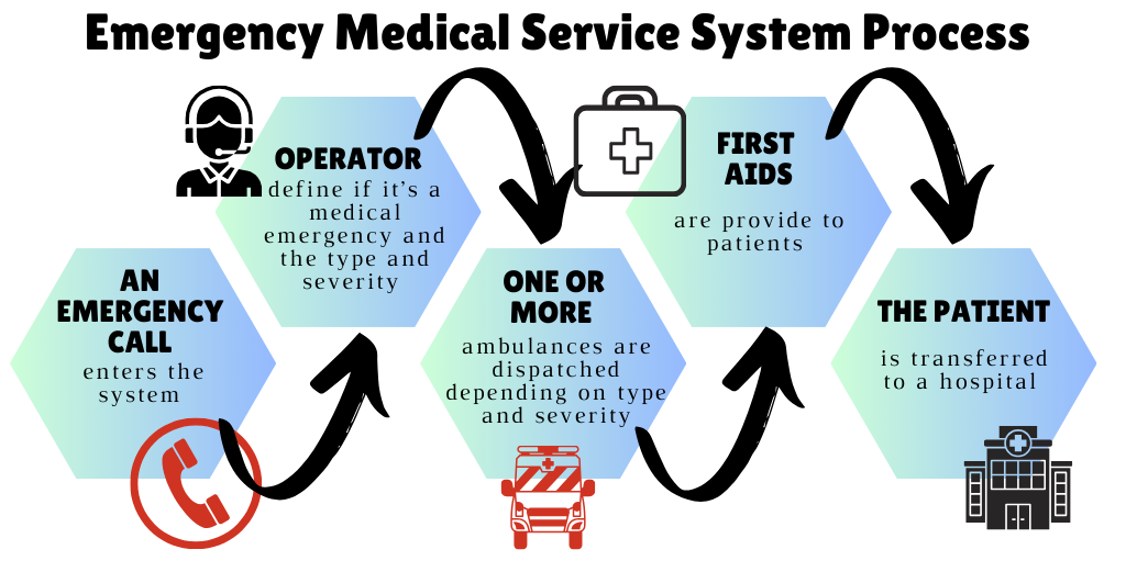
\includegraphics[width=0.82\linewidth]{EMS_System.png}
    \caption{An Emergency Medical Service System Process.}
    \label{fig:ems}
\end{figure}

EMS systems have significantly impacted operational research and medical investigations in the last decades \cite{ball1993reliability, olave2021modeling, aboueljinane2013review}. Scientists are concerned about the impact of calls emergency' average response time for attending a patient who suffers a medical incident. Moreover, the cost of buying material resources, medical vehicles, or building a new medical center, among other things, can limit the service to patients~\cite{hulshof2012taxonomic}. Lack of human and material resources can cause insufficient attention in patients \cite{kabene2006importance, ahlenius2017patients, garcia2018patient}.

The most studied problem is reducing the average response time when an emergency call arrives at a call center and someone needs medical attention \cite{blackwell2002response}. 
The objective is to provide, as soon as possible, the initial treatment for a patient that has a medical problem caused by an accident, a trauma, or a natural disaster to reduce patients' mortality. For short response time, more likely people survive. Another objective that EMS system problems consider is to maximize coverage to attend all emergency calls that enter the system \cite{chanta2014improving}. Also, some problems exist that consider improving the patients' survival or reducing the patients' mortality \cite{zaffar2016coverage}. 

%There exist different types of problems. Various focus on statics systems, where the decisions are fixed after they are taken. Others are dynamic~\cite{brotcorne2003ambulance}, where decisions change throughout time passing or after a change on the system, for example, when a call is received. Many investigations focus their problems on solving optimal locations of their ambulances to improve the system. In contrast, others want to obtain optimal policies to decide which ambulance or ambulances are the best to attend the emergency calls received.

%EMS systems have different strategic, tactical, and operational types of plan\-ning~\cite{galvao2008emergency}. Strategic planning focuses on long-term decisions, such as fixed potential locations or the acquisition of resources~\cite{aboueljinane2013review}. Tactical plannings made decisions for a middle time, such as locating ambulances at potential sites or planning which is the best option to dispatch an ambulance for all emergency calls types. Finally, operational planning takes decisions in a short time. These decisions are made frequently when a call enters the system and are divided into online and offline decisions. Online decisions are taken over the full service of a call, and offline decisions are taken when a call is received following the plannings made at tactical plannings, for example, to decide which ambulance will send to attend to the pa\-tient~\cite{hulshof2012taxonomic}.

Our interest is in the EMS systems of Mexico. In Mexico exists the \text{\text{9-1-1}} number controled by the C-5 organization (Centro de Coordinación Integral, de Control, Comando, Comunicaciones y Cómputo del Estado), which receives e\-mer\-gen\-cy calls. Some calls are for medical emergencies, others for police e\-mer\-gen\-cies, and others for fire emergencies. When a call enters the system, and an operator decides that it is a medical emergency, the operator has to determine if it is necessary to send an ambulance or not. Also, a doctor can continue the call to guide the person on the phone if the patient needs immediate attention while the ambulance arrives. Then the paramedics can attend to the patient and transfer the patient to a hospital~\cite{911_op}.

%The problem in our country is that more than one service provider is involved in the \text{\text{9-1-1}} system. The two most important are CRUM (Centro Regulador de Urgencias Medicas) and Red Cross. There exists in some states the Proteccion Civil and the Green Cross too, but CRUM controls them. Also, other private organizations exist, but they are not involved in the \text{\text{9-1-1}} system. That is one reason why an uncoordinated system exists in our country. CRUM is part of the government, and they control the public ambulances, while Red Cross is a private organization. Each service provider decides where to locate their ambulances without consulting the other. Furthermore, when an ambulance is needed to attend an emergency call for \text{\text{9-1-1}}, CRUM has preferences because Red Cross has its private number where people can call for medical attention. Red Cross dispatch ambulances that are supposed to be available in \text{\text{9-1-1}} systems for its direct emergency calls.We could improve this uncoordinated system if each service provider made its decisions considering others. Moreover, the system has the problem of queues at hospitals, which delays the patients' attention. Since the pandemic for Covid-19 started, some hospitals attend only Covid-19 patients. That causes the rest of the hospitals to have more demand than before the pandemic. So the ambulances from the \text{\text{9-1-1}} system are busy longer than before, and it has to be considered to improve the EMS system in Mexico.

We propose a two-stage stochastic programming model with recourses for ambulance location and dispatching, considering two service providers to obtain a coordinated EMS system to solve those problems. The following sections present the background investigations about EMS sys\-tems (Chapter \ref{cap:back}) and the usually used models. We describe the problem and factors that affect the EMS system in Mexico (Chapter \ref{cap:problem}). Also we describe (Chapter \ref{cap:assess}) the instance generation and experimental assessments. Then, we solve the problem and define the model (Chapter \ref{cap:Exp}) used to do the experiments. Finally, we show conclusions (Chapter \ref{cap:concl}) that we obtain from experiments described in the previous section, in this section we also propose a future work.

\section{Motivation}
Our interest is to improve the Emergency Medical Service System in Mexico, par\-ti\-cu\-lar\-ly in Nuevo León. World Health Organization (WHO) establishes that it has to be four ambulances per one thousand habitants, which is not available in the states throughout our country.

Due to the lack of available ambulances, emergency calls are answered late. However, buying more ambulances so that there are a greater number of them available to distribute is not an option. Improving the distribution of ambulances, and locating and dispatching them in a better way, could improve the EMS systems.

%Our interest is to improve the Emergency Medical Service System in Mexico. This system has different characteristics than others that have been studied. Especially in Mexico, public and private organizations work together, but they do not communicate what others do to make their decisions. 

%Also, since the Covid-19 pandemic in Mexico started, fewer hospitals are attending general medical emergencies, and ambulances do queues outside the hos\-pi\-tals waiting for patient attention due there are no available rooms for new patients. 

\section{Problem Description}
%\textbf{Yo creo que al decirlo asi es como que el EVCP es un problema conocido que YA existe, lo cual no es cierto... Creo seria emjor que abordamos un problema sobre EMS y en todo caso, el problema particular de nuetsro paper lo denotamos o bautazamos como EVCP... reescribop el abstract para que lo vean...}
%We address a problem for EMS systems, focused on Mexico and Latinoamerican countries, which we denoted as Emergency Vehicle Covering and Planning (EVCP) problem. This problem locates a limited number of two heterogeneous types of ambulances in different city points and dispatches them to the emergency scenes, considering the uncertainty of the emergency locations, to maximize the emergency total and partial coverage and the response time in which the patients receive medical first aids. We propose a novel two-stage quadratic stochastic program for the EVCP problem that locates the limited number of heterogeneous types of ambulances in the first stage. In the second stage, the dispatching of the ambulances to accidents is determined. The EVCP stochastic model allows partial coverage of the accidents by the ambulances based on a decay function. Instead of decomposing the stochastic model, we propose a location-allocation methodology that relies on the solution in an auxiliary surrogate model, which is faster to solve. The location of the ambulances obtained by this surrogate model is input to the original model. Experimental results show that we obtain high-quality solutions in a reasonable time.
We address a problem where we have to locate a limited number of two heterogeneous types of ambulances in different city points and dispatch them to the sites where accidents occur.  Our problem considers uncertainty of the accident (demand) points. Our goal to maximize the total and partial coverage and the response time in which the patients receive medical first aids. We propose a two-stage quadratic stochastic program for this problem. In the first stage, the location of the limited number of two types of ambulances is decided. In the second stage, the dispatching of the ambulances to accidents is determined. This stochastic model allows partial coverage of the accidents by the ambulances based on a decay function. Given the model is intractable even for medium-sized instances, we propose a location-allocation methodology that relies on the solution of an auxiliary surrogate model, which is faster to solve. This location-allocation heuristic consists of two phases.  In the location phase, the location of the ambulances is obtained by solving the surrogate model.  Then, this information is the input for the allocation phase, where the original model is solved. Experimental results show the effectiveness and efficiency of this proposed approach, obtaining high-quality solutions in reasonable times.

%The Uncoordinated Emergency Medical Service System (UEMSS) Problem is focused on improving an EMS system that involves more than one service provider. We have factors that affect service provider decisions for this system that we discuss below. We called patients at people who need some medical attention due to an accident or a medical condition that affects the person's health. There are some demand points where someone made an emergency call because the patient needs medical attention. Also, some potential sites are spaces in the zones attending to the EMS system where ambulances can be located in the system.

%An uncoordinated EMS system has more than one service provider involved in the emergency number system to attend emergency calls. These service providers have a certain number of ambulances available for patients' medical attention. The total ambulance available number may vary depending on the day of the week and the period time of the day. The ambulances need some material resources but also human resources. The EMS system has to consider the paramedics attending to the patients. If there are not enough paramedics for the total ambulances, not all the ambulances are available for the system. 

%There are two different ambulance types: basic life support (BLS), which attend not severity accidents, and advanced life support, which attend severity accidents. Each ambulance has a response time for travel from the potential site where it is located to the demand point where the patient will be served. Also, hospitals know where patients will move after their attention. Paramedics need to know if a patient has health insurance to decide where a patient will be transferred. 

%For our UEMSS Problem, we consider scenarios with information about ac\-ci\-dents at the demand point. Each element of one scenario has information about how many BLS and ALS need each demand point, and the sum of ambulances needed can be one, two, or three ambulances for point.

\section{Hypothesis}
This investigation hypothesizes that we can model the Emergency Vehicle Covering and Planning problem as a stochastic programming model with resources based on different scenarios. These scenarios consider accident types in each demand point; many of them can help know what to do when a situation occurs in the \text{9-1-1} system. The ambulance location and dispatching in the system are optimized.

%This investigation hypothesizes that we can model the Uncoordinated Emergency Medical Service System Problem as a stochastic programming model with resources based on different scenarios. These scenarios consider accident types in each demand point; many of them can help know what to do when a situation occurs in the \text{9-1-1} system. The model includes characteristics of each service provider, and the decisions are taken coordinate considering these characteristics. The ambulance location and dispatching in the system are optimized.


\section{Objectives}
This investigation aims to improve an Emergency Medical Services System con\-si\-de\-ring partial coverage. The main idea is to obtain an optimal ambulance location and optimal policies for ambulance dispatching. The system that we consider for the problem to solve includes different factors that affect the system. Those factors are:
\begin{itemize}

\item Various types of accidents and variations on maximal response times depending on accident types; 

\item Different ambulances types, which are ambulances for basic life support (BLS) and ambulances for advanced life support (ALS);

\item And variation in demand points depending on the day of the week and the hour of the day, which can be considered making different scenarios.

%\item And queues at hospitals for patients' attention that increase the service time for an emergency call.

\end{itemize} 

The objective for solving the problem is to create a scenario-based stochastical programming model with resources considering more than one service provider in\-vol\-ved in the system to attend incoming emergency calls. 


\section{Scientific dissemination}
Over these years, this investigations has been presented in different national and international conferences. National conferences are CSMIO (Congreso de la Sociedad Mexicana de Investigación de Operaciones) in the years 2021 (online), 2022, and 2023; CSMM (Congreso de la Sociedad Matemática Mexicana) in the years 2021 (online) and 2023. Also we participated in ELAVIO (Escuela Latinoamericana de Verano en Investigación Operativa) in the year 2022; the \textit{Coloquio VNL de Gráficas, Combinatoria y sus Aplicaciones} in the year 2023 and some seminars in one middle school (Preparatoria 7 Puentes) in the year 2022 and two high schools (Facultad de Ciencias Físico Matemáticas and Facultad de Ingeniería Mecánica y Eléctrica), in the year 2021 and 2024, of the UANL (Universidad Autónoma de Nuevo León). The international conferences are CLAIO (Latin-Iberoamerican Conference on Operations Research) in the year 2024; and the INFORMS ALIO-ASOCIO International Conference also in the year 2024.

An article of this investigation has been accepted.  


\chapter{Background}\label{cap:back}

Emergency Medical Services (EMS) systems provide basic but urgent in-situ medical care for people who suffer a medical incident and then transport patients to hospitals \citep{aringhieri2017emergency, belanger2019recent, reuter2017logistics}. When scientists talk about EMS systems, many terms explain the problem. Two of these terms are demand points and potential sites. Demand points are sites where an emergency call is usually done. Commonly, there is a different demand for each point depending on the number of calls made within a period. Potential sites are places where a vehicle (ambulance) could be located if necessary to cover some demand points either statically or dynamically.

The first phase of an EMS is the response to an emergency call by an operator that identifies the emergency type: accident, medical, security, fire, etc. The second phase is dispatching one or several ambulances to the emergency scene to provide urgent medical care. Some emergency situations, such as a multiple-car accident, may involve several people; thus, more than one ambulance could be needed. More\-over, different types of ambulances may be required in an emergency: Basic Life Support (BLS), usually with two Emergency Medical Technicians (EMTs), and Advanced Life Support (ALS) units with an EMT, an advanced EMT, and one or two Paramedics. The third phase involves the paramedics' treatment of the patients and transporting them to a hospital~\citep{aringhieri2017emergency}. 

EMS systems in developing countries, as is the case in Mexico, lack around 30-60\%\footnote{Anonymous interviews done by the authors.} of the number of ambulances suggested by the World Health Organization (WHO), which is at least four ambulances per 100,000 people \citep{braun1990characteristics}. For the Red Cross, an EMS operating with this small number of ambulances is considered similar to a war situation$^1$. Thus, one of the main contributions of this work is to deal with the problem of deciding if an emergency will be totally or partially covered. Sadly, some emergencies may remain uncovered by an emergency unit. 

Commonly, emergency vehicle planning problems' main objective is to reduce the average response time of a patient's initial treatment given by a paramedic in an emergency \citep{amorim2019traffic, bandara2012optimal,toro2013joint, toro2015reducing}. Indeed, the quickness and the number of ambulances dispatched to the accidents are crucial. Each ambulance has a response time for travel from the potential site where it is located to the demand point where the patient will be cared for. Every minute of treatment delay in a cardiac patient reduces the survival probability by 24\% \citep{o2010role}.  

There are many models to solve the problems of EMS systems divided into deterministic, probabilistic, and stochastic problems, which use different solution methods to solve them \cite{brotcorne2003ambulance}. The first problems that we studied are the statics. 

\section{Static models}

These models are used to solve a system that only considers a particular point in time. When these models are used to solve EMS systems, it refers to allocating ambulances that will not be moved from the base. 

There are two early models for statics problems: Location Set Covering Model (LSCM) and Maximal Covering Location Problem (MCLP), which are problems focused on covering the maximal demand points in the entire zone. However, over time these problems evolved according to the needs of the Emergency Medical Services, as will be defined below.


\subsection{Deterministic models}

Deterministic models were proposed to solve static problems because sometimes the emergency calls need to be attended for different vehicle types. Most of them are covered once, like the Backup Coverage Problem (BACOP) or the Double Standard Model (DSM), which use two different radii of coverage \cite{li2011covering}. Alternative deterministic models are the tandem equipment allocation model (TEAM) or the facility-location equipment-emplacement technique (FLEET), which consider two types of vehicles (one for basic life support and another for advanced life support), or the fact that sometimes more than one ambulance has to be located on a potential site to maximize that a demand point is covered twice. 

In the thousands was introduced by Berman et al. \cite{berman2003gradual} a decay function to classify coverage as full, none, and partial coverage in a generalized MCLP model. They added a weighted demand for each node covered, considering the distance between facilities and demand points. The objective aims to maximize the total demand weight covered by all facilities when a determined number of facilities are located.

A year later, \cite{karasakal2004maximal} introduced partial coverage to the MCLP problem. This problem aims to maximize coverage level for all demand points deciding where to locate a certain number of facilities within the available potential sites. The model was based on a $p$-median formulation and classified coverage into three levels: totally covered, partially covered, and not covered. They defined a decay function monotone decreasing according to the distance between the facility and demand point for partial coverage. The distance between a facility and a demand point has to be less or equal to the maximum full coverage distance established to consider total coverage. Demand points are considered not covered for a facility if the distance between it and the demand point is greater or equal to a maximum partial coverage distance. To solve large-size problems, they used a Lagrangian relaxation.

A decade after, Wang et al. \cite{wang2016new} used an extension of the MCLP Problem to maximize coverage for fire emergencies establishing a travel cost between potential sites and demand points. This extension considers a partial distance and quantity coverage for multi-type vehicles to locate and dispatch them. Partial distance is calculated with a decay function, which decreases according to the vehicle response time increase. Quantity coverage determines if an emergency is completely served or not, comparing the number of vehicles dispatched with the necessary quantity. For this problem, they have to consider demand priority to know where vehicles must be located and the patient's classification to decide how to dispatch them.

As an extension of DSM, Dibene et al. \cite{dibene2017optimizing} created the Robust Double Standard Model. They added demand scenarios to the original DSM problem. These scenarios divide weeks into workdays and weekends, divided into four periods: night, morning, afternoon, and evening. They added eight scenarios applied to optimize the Red Cross Tijuana, Mexico system, increasing the coverage of demand points to more than 95\% locating ambulances on different points of the city that are not the original bases.  

For us, it is imperative to gather all this information for our project as it provides insights into the different accident coverage types and the improvement for ambulances location. A thorough understanding of these models and their effectiveness will enable us to optimize mainly our ambulance location strategies.

\subsection{Probabilistic models}

In the eighties, some researchers thought about problems involved with probabilities. One of these probabilities involved in EMS systems is the probability of an ambulance being busy responding to an emergency call. This probability is called the \textit{busy fraction}. The maximum expected covering location problem (MEXCLP) uses this probability. An extension of this model is the TIMEXCLP which considers travel speed variations during the day. Another extension is the adjusted MEXCLP model (AMEXCLP), which considers different busy probabilities for each potential site to locate ambulances. All these models can use the hypercube queueing model to calculate the busy fraction \cite{galvao2008emergency}.

Other models were proposed to maximize the coverage of the demand points with a probability $\alpha$ used to calculate the busy fraction; one of them is the maximal availability location problem I (MALPI), which considers the busy fraction is the same for all potential sites. Another model is the MALPII which uses the hypercube model to assume different busy fractions for each potential site.

There exist more probabilistic models created in the nineties. The first is an extended version of the LSCM called Rel-P; this version considers that more than one ambulance can be located at the same potential site, but each potential site has a probability to has ambulances that are available to respond to a call and consider the probability of the busy fraction too. 

The second model is the two-tiered model (TTM), which consider two types of vehicles to allocate at potential sites (BLS and ALS) considering two different coverage radii and having an associated probability for the combination of how many ALS vehicles can be located at the radius A, how many ALS can be located at the radius B and how many BLS vehicles can be located at the same radius B for each demand point. 

Laura Albert and Maria Mayorga researched the EMS systems of Hanover, Virginia. All these investigations about Hanover, Virginia, were applied to this county to obtain practical solutions, but all models can be used to any other EMS system changing data inputs.

The first research is focused on considering a new approach to calculate the response time threshold (RTT), a class of EMS performance measures \cite{mclay2010evaluating}. The approach uses the patient survival rate considering that patients have a cardiac arrest and random response times that depend on the distance between demand points and potential sites instead of patient outcomes, which is most used. Then, they use these measures on a hypercube model to evaluate different RTTs needed to input a model that considers fire stations and rescue stations to be potential sites where ambulances could be located distributed on Hanover's rural and urban areas. This model optimizes the location of ambulances on potential sites to maximize patient survival. 

Later, Albert and Mayorga et al. used the performance measures as an input of the performance measure dispatching problem. According to survival patient rate, they used a Markov decision process that identifies the best and most robust RTT to maximize the covering level, prioritizing patient location. The research concludes that the optimal survival rate is obtained when the system has an eight minutes RTT \cite{mclay2011evaluating}. However, this time for RTT does not apply to Hanover because of the number of the ambulance that they have, so they started a pilot program called quick-response vehicle to have more vehicles for patient attention obtaining a nine minutes RTT, these new vehicles are as ALS vehicles without transporting patients to the hospital, only attending patients at the scene and BLS ambulances transport patients if is necessary \cite{mclay2012hanover}. The idea of including these quick-response vehicles is to minimize the need to use ALS ambulances.

When talking about optimizing EMS systems, one can also speak about dis\-pat\-ching. Bandara et al. \cite{bandara2012optimal} considers demand priorities for the different emergency calls arriving at the system. The objective is to maximize the patient's survival probability when an ambulance is dispatched to demand points, calculating a reward for each dispatch. They used a Markov Decision Process model formulation to determine the optimal dispatching strategies for an EMS system.

\citet{toro2013joint} involves location and dispatching decisions for EMS vehicles in the same mathematical model with two focuses, minimizing the mean response time that takes since an emergency call is received and maximizing the expected coverage demand, using a continuous-time Markov process to balancing flow e\-qua\-tions needed to control the busy fraction for each ambulance. Balancing these equations takes exponential time, and authors consider a genetic algorithm to obtain some solutions and combine them to create new solutions to reduce the computational time. This genetic algorithm was applied to Hanover, Virginia, and when they have mid-size problems, the nearest dispatch rule is the best solution. It can vary depending on the zone where it is applied.

\citet{amorim2019traffic} involve a simulation inputting an initial solution to decide if ambulances have to stay at the potential sites establishes when the mathematical model is solved or if some of them have to be moved to another potential site. To decide how to proceed, they used different day's period times when traffic in the city is changing on each week's days, which they called \textit{scenarios}, to maximize the patient's survival. 

Transitioning from probabilistic models to scenario-based models in the management of EMS systems is imperative, as scenarios provide a more robust framework for addressing uncertainty. Probabilistic models frequently require assumptions regarding the likelihood of various events, such as the busy fraction of ambulances, which can be challenging to estimate accurately and may not adequately capture real-world complexities. In contrast, scenario-based models allow for the incorporation of various demand and traffic conditions, enabling more realistic and flexible planning. By utilizing scenarios, researchers can ensure a more reliable and adaptive emergency response system, improving also dispatching decisions, as we can see in the next section.

\subsection{Stochastic models}

Recently, ambulance location, allocation, and dispatching problems involved un\-cer\-tain\-ty at demand points to have a more realistic model. This uncertainty is caused because it is impossible to know when the system will receive an emergency call.

In 2017, Boujemaa et al. \citep{boujemaa2018stochastic} proposed a two-stage stochastic model with recourse. The model's first stage determines where to open ambulance stations with a fixed cost for opening them. For the second stage, allocation is determined considering the expected traveling cost from ambulance stations to de\-mand points. A demand point is considered covered if an ambulance station is within a threshold value. And some important factors that they included are two different demand types: life-threatening calls and non-life-threatening calls; two ambulance types: ALS and BLS; and scenarios structured by two data for each demand point: number of life-threatening calls and number of non-life-threatening calls, respectively. This problem minimizes the ambulance location-allocation cost and is solved by a Sample Average Approximation (SAA) algorithm that allows computing lower and upper bounds for problem solutions and providing the corresponding optimality gaps.

Later, Bertsimas and Ng \cite{bertsimas2019robust} implemented stochastic and robust formulation for ambulance deployment and dispatch for a problem constructed as a graph. These formulations were compared with MEXCLP and MALP problems and aimed to minimize the fraction of late-arrivals without requiring ambulances to be repositioned, sending to demand points the closest available ambulance, and maintaining a call at a queue if there are no ambulances available at the system. The demand has the problem's uncertainty, which was constructed by four demand types: single for each demand point, local for the demand point and the nearest points, regional for a region of the entire zone, and global for the whole area. They determined a deterministic equivalent model to solve the stochastic formulation, and for the robust formulation, they did a column and constraint algorithm.  

Recently, Yoon et al. \cite{yoon2021stochastic} studied a two-stage stochastic problem for locating and dispatching two types of emergency vehicles: ALS and BLS. The first stage locates the ambulances at potential sites, while the second stage dispatch ambulances from places where they were located to demand points when a call arrives. The objective is to maximize the expected coverage considering a penalty when a call is not serviced. One difference from other problems is that the system manages multiple emergency call responses, divided into high priority and low priority calls. Any vehicle type can serve low priority calls. However, high-priority calls have two options for the service: the first option is that these calls can be responded to an ALS ambulance. The second option is that a nearby BLS ambulance can service the call first, followed by an ALS ambulance that is not necessarily closed. An SAA deterministic equivalent formulation solved this problem for small data, while a Branch-and-Benders-Cut Solution solved a large-scale problem. And they did another problem version considering non-transport vehicles which can attend patients without translating them to hospitals.

Some works propose stochastic programming models based on call-arrival sce\-na\-rios as a bundle of calls, the total number of emergency calls in each demand node during a given period. As we do in this work, a two-stage stochastic program deploys the ambulances in the first stage and dispatches them to respond to demand in the second stage. \citet{beraldi2009probabilistic} and \citet{noyan2010alternate} induce a reliability approach by using probabilistic constraints. \citet{nickel2016ambulance} minimize the total cost of locating the ambulances while assuring a minimum coverage level. By considering a bundle of calls, they address the volume of calls during a short period, such as the Friday night hours. \citet{bertsimas2019robust} implemented stochastic and robust formulations for ambulance deployment and dispatch to minimize the fraction of late arrivals without requiring ambulances to be relocated, sending to demand points the closest available ambulance, and maintaining a call at a queue if there are no ambulances available at the system. 

\section{Heuristics}
AGREGAR AQUÍ INFORMACIÓN SOBRE ESTOS PROCEDIMIENTOS

All the information gathered will be utilized collectively to formulate a novel problem that can integrate and utilize the previously mentioned knowledge and strategies. This approach aims to provide a comprehensive and advanced method for optimizing EMS systems.


%\section{Dynamic models}

%A dynamic model on EMS systems is used to locate and relocate am\-bu\-lan\-ces from their base to another if necessary for real-time. These models are called dynamic because the system is changing over time. Usually, the \textit{real time} that is used in an EMS system is when an emergency call is received. 

%One of these models is the Dynamic Double Standard Model at time $t$, an extension of DSM \cite{belanger2019recent}. Some differences for this model are that every time $t$, am\-bu\-lan\-ces are moved to another base to cover once demand points at a minimum probability $\alpha$. There is a cost to move the ambulances from its base to another potential site. This cost is a penalty in the objective function. 

%Another model of these models is the dynamically available coverage location (DACL). For this model, the system changes when the demand of demand points changes during the day and uses the hypercube theory to calculate the busy pro\-ba\-bi\-li\-ty for potential sites every time. 

\section{Contribution}

%Our opportunity area for this thesis is to analyze a problem for maximizing coverage considering null, partial and full coverage. We use different levels to evaluate a demand point as partially covered. It depends on the distance between the potential site and the demand point, calculated with a decay function. Also, we calculate how many ambulances of each type were sent to service an accident. 

%We propose a two-stage stochastic problem with recourse where the first stage is for locating ambulances at potential sites. The second stage determines how to dispatch them to demand points when an accident occurs. 

%ALS and BLS vehicles are considered for this problem. Any ambulance type can serve accidents that need BLS ambulances, but accidents that need ALS ambulances can be only served by ALS ambulance type. For our scenarios, we have two data: the first is for the number of BLS vehicles needed at the demand point, and the second is the quantity of ALS vehicles required for the same demand point.

%Additionally, we propose an intelligent feedback to obtain ambulance location in a faster time that will be use as an input for the stochastic programming model that decides how to dispatch them to demand points.

%In the literature, we do not find a system where exists more than one service provider and considers all factors that we assume. However, it is essential to study it because public and private service providers are involved in Mexico. Sometimes, there is a conflict with them when dispatching is done for an accident. So we want to consider both of them to obtain a coordinated EMS system. 

The novelty in this work resides in additionally maximizing the coverage of emergency situations and considering different types of ambulances. When a BLS ambulance is dispatched to an emergency requiring an ALS, it may reduce the patient's survival. Thus, this work considers that ALS ambulances can be used as BLS units, but the contrary is not allowed~\citep{bakalos2011advanced}. There are a few works that deal with different types of ambulances as we do in this work. \citet{mclay2009maximum} determines how to optimally locate and use ambulances to improve patient survivability and coordinate multiple medical units with a hypercube queuing model. \citet{grannan2015maximum} determine how to dispatch multiple types of air assets to prioritized service calls to maintain a high likelihood of survival of the most urgent casualties in a military medical evacuation by a binary linear programming model. In \citet{yoon2021stochastic}, two types of vehicles are considered, but one of them is a rapid one that cannot offer the first care services of an ambulance. Moreover, neither of these works considers partial covering of the calls. 

We denote our problem as the \textit{Emergency Vehicle Covering and Planning} (EVCP) problem which consists of locating the limited number of two heterogeneous types of ambulances in different city points and dispatch them to the accident points, considering the uncertainty of the accident points, so as to maximize the coverage (even if partially) with short medical first aid response time. Usually, the location and dispatching decisions are made separately \citep{belanger2019recent, dibene2017optimizing, wang2012modeling}. In the EVCP problem, these two interrelated decisions are simultaneously determined as done by \citet{toro2015reducing, ansari2017maximum, amorim2019traffic}. 

We propose a novel two-stage stochastic program for the EVCP problem. The stochastic program locates the limited number of heterogeneous types of ambulances in the first stage, and in the second stage, the dispatching of ambulances to accidents is determined. The EVCP stochastic model allows partial coverage of the accidents by the ambulances based on a decay function \citep{wang2016new}. Similarly to \citet{yoon2021stochastic}, we generate the call-arrival scenarios by sampling from emergency call logs to use them in the second stage of our stochastic model. In this manner, we address the volume of calls during a short period, such as Friday night hours. Thus, time is not explicitly measured, and it is assumed that a vehicle can be assigned only once during this high ambulance demand period~\citep{zhou2015spatio}. \citet{boujemaa2018stochastic} use a bundle of calls but do not consider a heterogeneous ambulance fleet. 

Another contribution of this work is the methodology to solve the EVCP stochastic model. Indeed, the proposed model can only be solved for relatively small instances with a restrictive number of scenarios. Thus, instead of decomposing the model with Bender's methods as it is usually done \cite{zhang2023multi, sung2018scenario}, we propose a location-allocation methodology \cite{shaw2022location, van2018demand} that relies on the solution in an auxiliary surrogate model, which is faster to solve. We name this method \textit{an intelligent feedback approach} because the location of the ambulances obtained by this surrogate model is used as input to the original model. Thus, we obtain high-quality solutions in a reasonable time with an off-the-shelf solver without complex decomposition techniques.

Some works use metaheuristic methods to solve their stochastic models. \citet{toro2013joint} integrate location and dispatching decisions for EMS vehicles to minimize the mean response time of an emergency call and maximize the expected coverage demand, using a continuous-time Markov process to balance flow equations that control the busy fraction of each ambulance. A genetic algorithm can solve mid-size instances. Some others, such as \citet{amorim2019traffic}, use simulation to decide if ambulances stay at the potential sites established by a mathematical model or must be moved to another potential site to maximize the patient's survival. They work on a complete day period while we focus on high-demand periods of some hours. Moreover, we do not need a metaheuristic due to the high-quality solutions that we obtained with the Intelligent feedback approach. However, we would like to propose a matheuristic to improve the solution obtained from this approach.


\chapter{Problem desciption}\label{cap:problem}%\label{sec:descr}%
The Emergency Vehicle Covering and Planning problem (EVCP) locates a limited number of two heterogeneous types of ambulances in different city points and dispatches them to the emergency scenes, considering the uncertainty of the emergency locations, to maximize the emergency total and partial coverage and the response time in which the patients receive medical first aids.

\section{Description and assumptions}\label{sec:description}

Let us formally describe the Emergency Vehicle Covering and Planning problem.
Let set $I$ include the possible demand points where patients may need medical attention in a city or region. This set can be very large, so we consider all the demand points observed in the historical data. In our case study, $|I|$ can be as large as 1500 demand points. Set $L$ provides the potential sites or ambulance stations where ambulances could be located, such as hospitals, firehouses, malls, or similar places where the ambulance and the paramedics can wait for emergency calls. We consider instances with up to 30 potential sites for the experimental results. Set $K$ contains the two types of ambulances available in the system: the BLS (labeled with index $k=1$) and the ALS ambulances (labeled with index $k=2$), which are limited by a known parameter $\eta_k$ for each type $k \in K$. These ambulances must be allocated to a potential site $l \in L$ and dispatched toward a demand point $i \in I$ if there is an emergency situation. 

The traveling time of any ambulance type from a potential site $l \in L$ to a demand point $i \in I$ is given by $r_{li}$. Ideally, ambulances should arrive in less than $\tau$ minutes in a life-threatening emergency. Usually, $\tau$ is a fixed value in the $[8,15]$ range. This work also considers that the emergency is not covered if an ambulance takes more than a maximum time $\tau_{\max}$ to arrive. In this case, sadly, the accident has probably been dealt with by other means. 

Since the aim of the EVCP problem is to reduce the response time of the patient's first medical aid, even if it is in a partial or late way, we define a benefit  decay function that only depends on the response time of a location $l\in L$ to any demand point $i\in I$:
   \begin{equation*}
       c_{li} = \left\{ 
        \begin{array}{lcc} 
            1 & \text{ if } & r_{li} \leq \tau, \\ 
            1- \frac{r_{li}-\tau}{\tau_{\max} -\tau}  & \text{ if }  & \tau < r_{li} < \tau_{\max}, \\       
            0 &   \text{ if }  & r_{li} \geq \tau_{\max} .
    \end{array} \right.
   \end{equation*}

\section{Information related to the scenarios}
   
The operational level is represented by a set of scenarios $S$ with a bundle list of arriving calls. Each scenario $s \in S$ represents a realization of accidents in the demand points.  Thus, a scenario is represented by the number and type of ambulances needed at each demand points.
%For each $s\in S$, we know the number and type of ambulances that should be dispatched to the emergency calls. 
Recall that an ALS ambulance can be sent instead of a BLS ambulance, but not the other way around. Thus, each scenario $s\in S$ indicates if there is an accident on a demand point $i \in I$ and provides the value $a_{ki}^s$ related to the number of required ambulances of type $k \in K$.  

For each scenario $s\in S$, let $I^s\subseteq I$ contain only the demand points $i\in I$ where ambulances are needed, that is, where $a_{ki}^s\neq 0 $ for any $k\in K$. We define five different types of ambulance coverage related to the response times cases for each demand point $i\in I^s$:
\begin{itemize}
    \item Total: the $a_{ki}^s$ required ambulances of each type $k$ are dispatched to $i$, and all arrive in less than~$\tau$ time.
    \item Total-late: the $a_{ki}^s$ required ambulances of each type $k$ are dispatched, but at least one arrives between $(\tau,\tau_{\max})$ time.
    \item Partial: at least one of the $a_{ki}^s$ required ambulances is not dispatched, for $k\in K$, but all the dispatched ones arrive in less than $\tau$ time.
    \item Partial-late: at least one of the $a_{ki}^s$ required ambulances is not dispatched, for $k\in K$, but at least one of the dispatched arrives between $(\tau,\tau_{\max})$ time.
    \item Null: none of the $a_{ki}^s$ required ambulances arrives in less than $\tau_{\max}$ time, for $k\in K$.
\end{itemize}

\begin{figure}[H]
    \centering
    %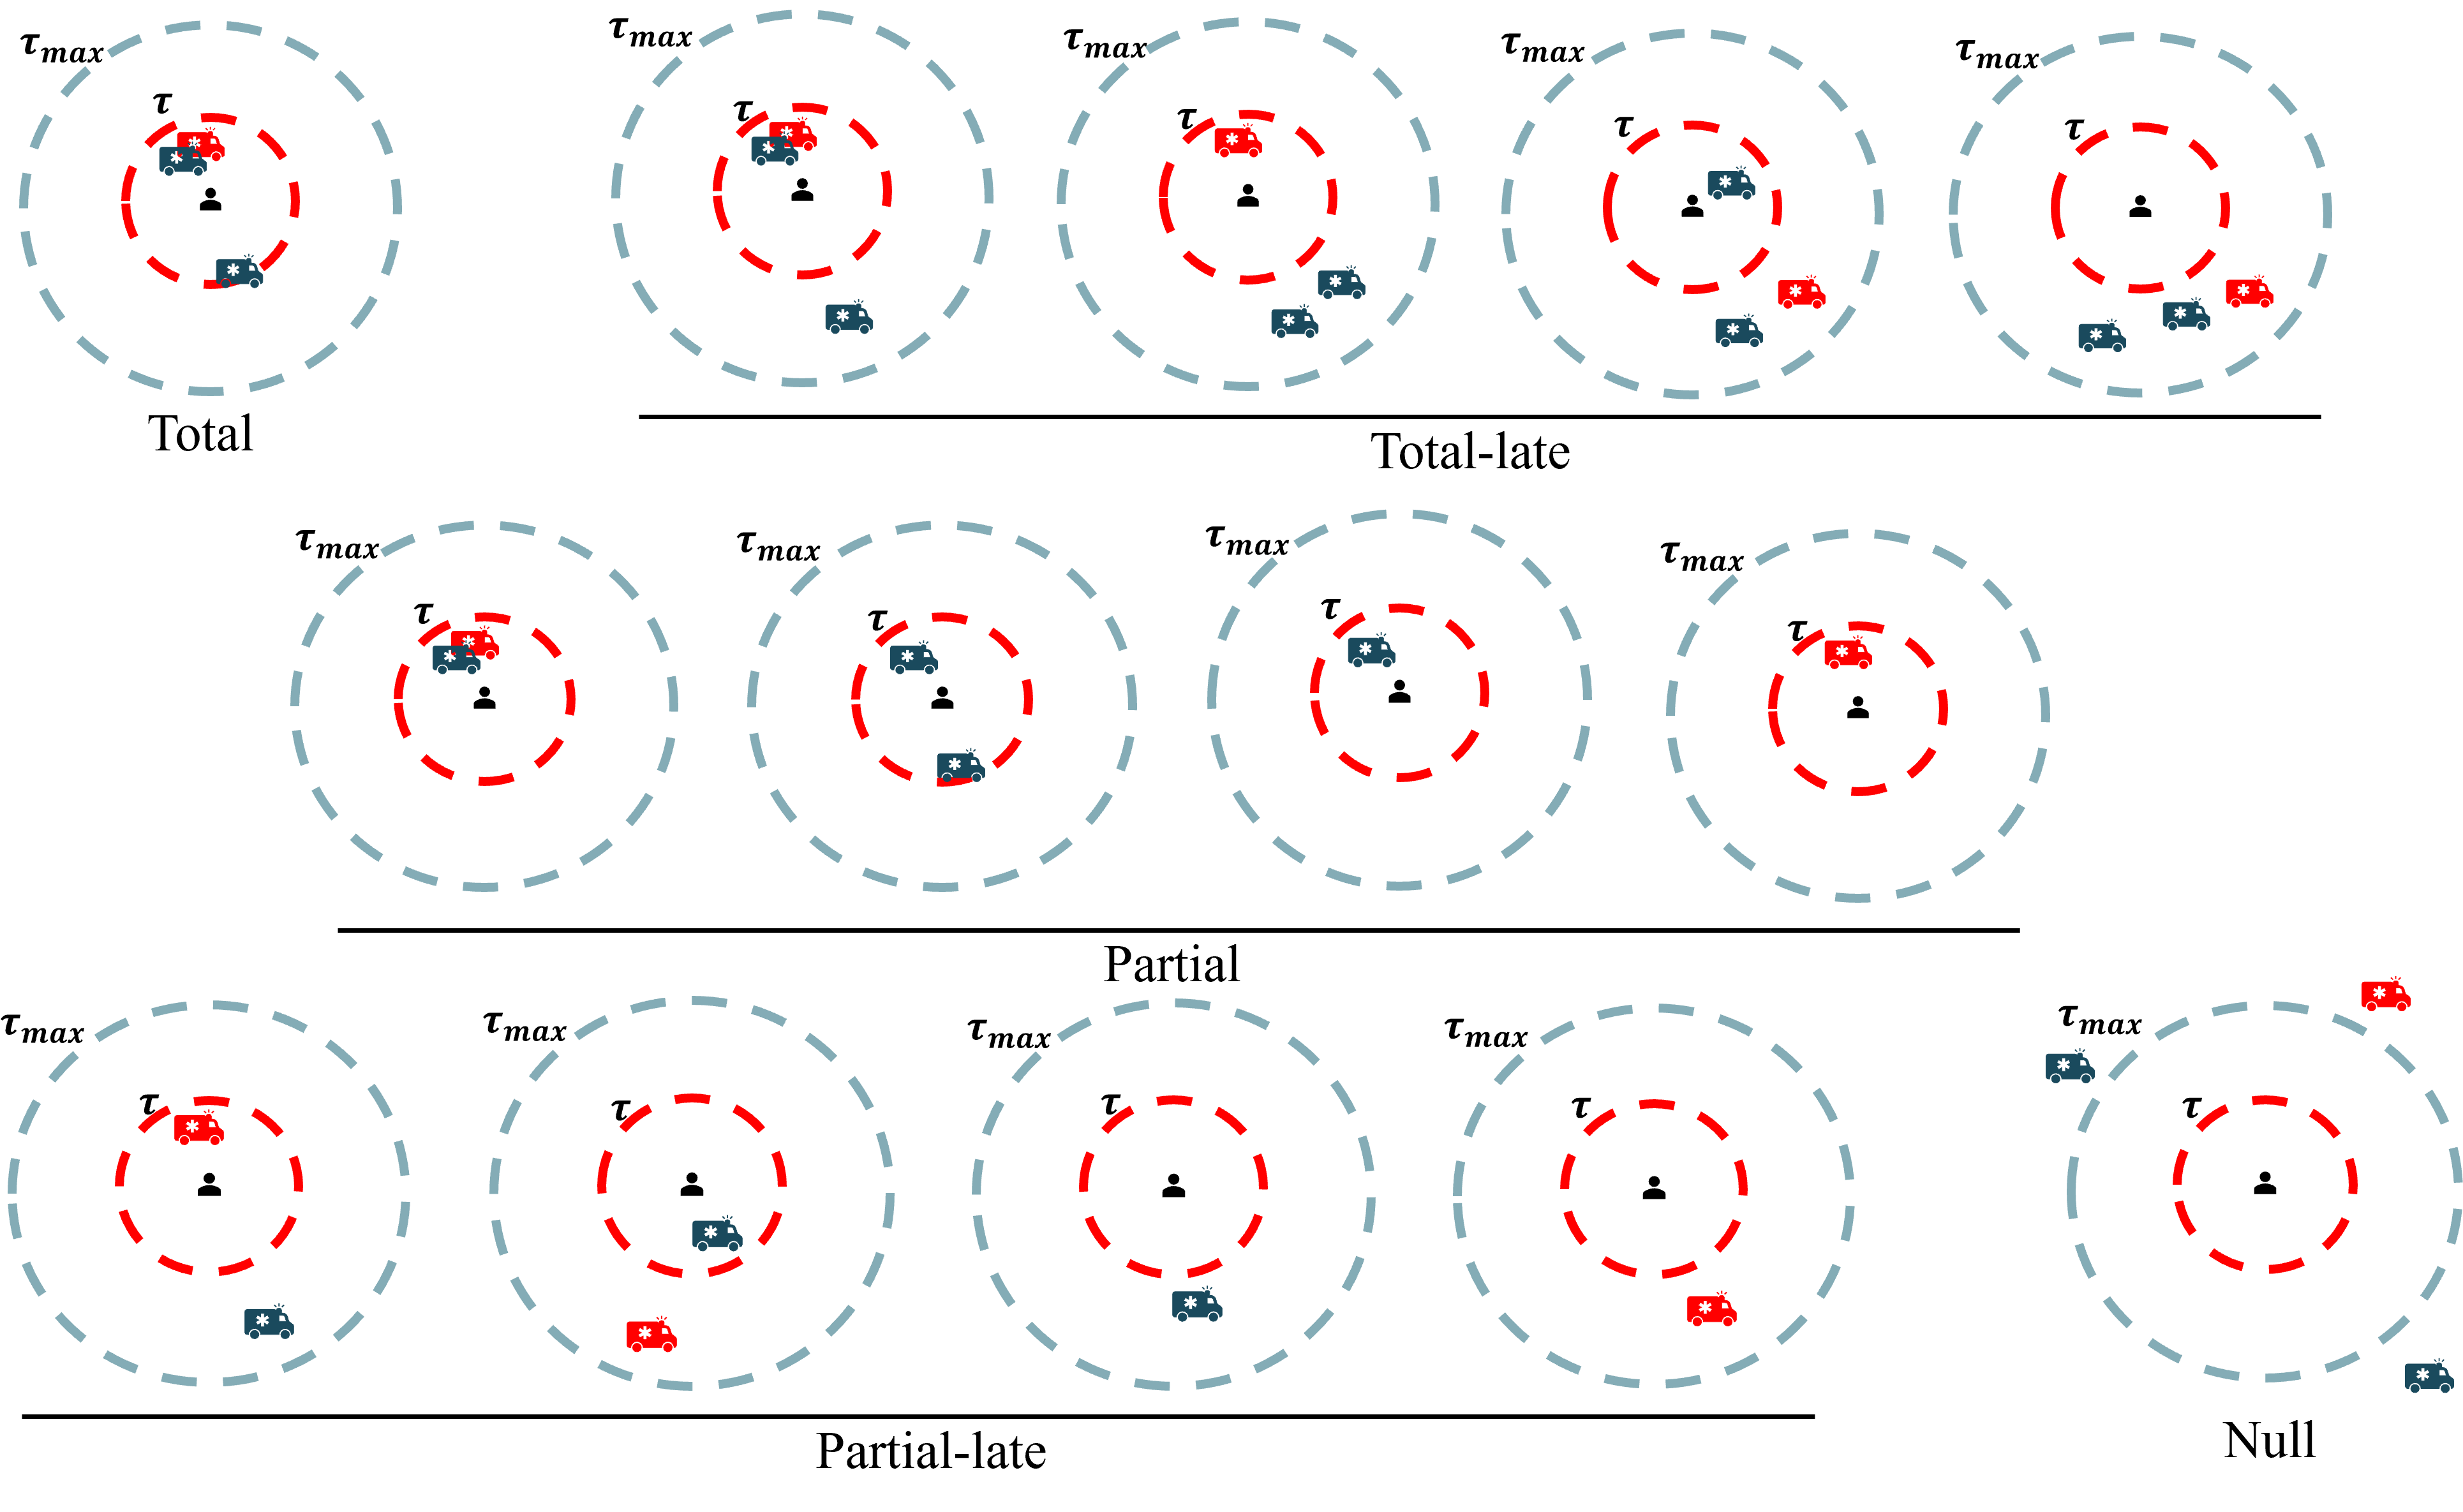
\includegraphics[width=0.97\textwidth]{figures/coverage-types.png}
    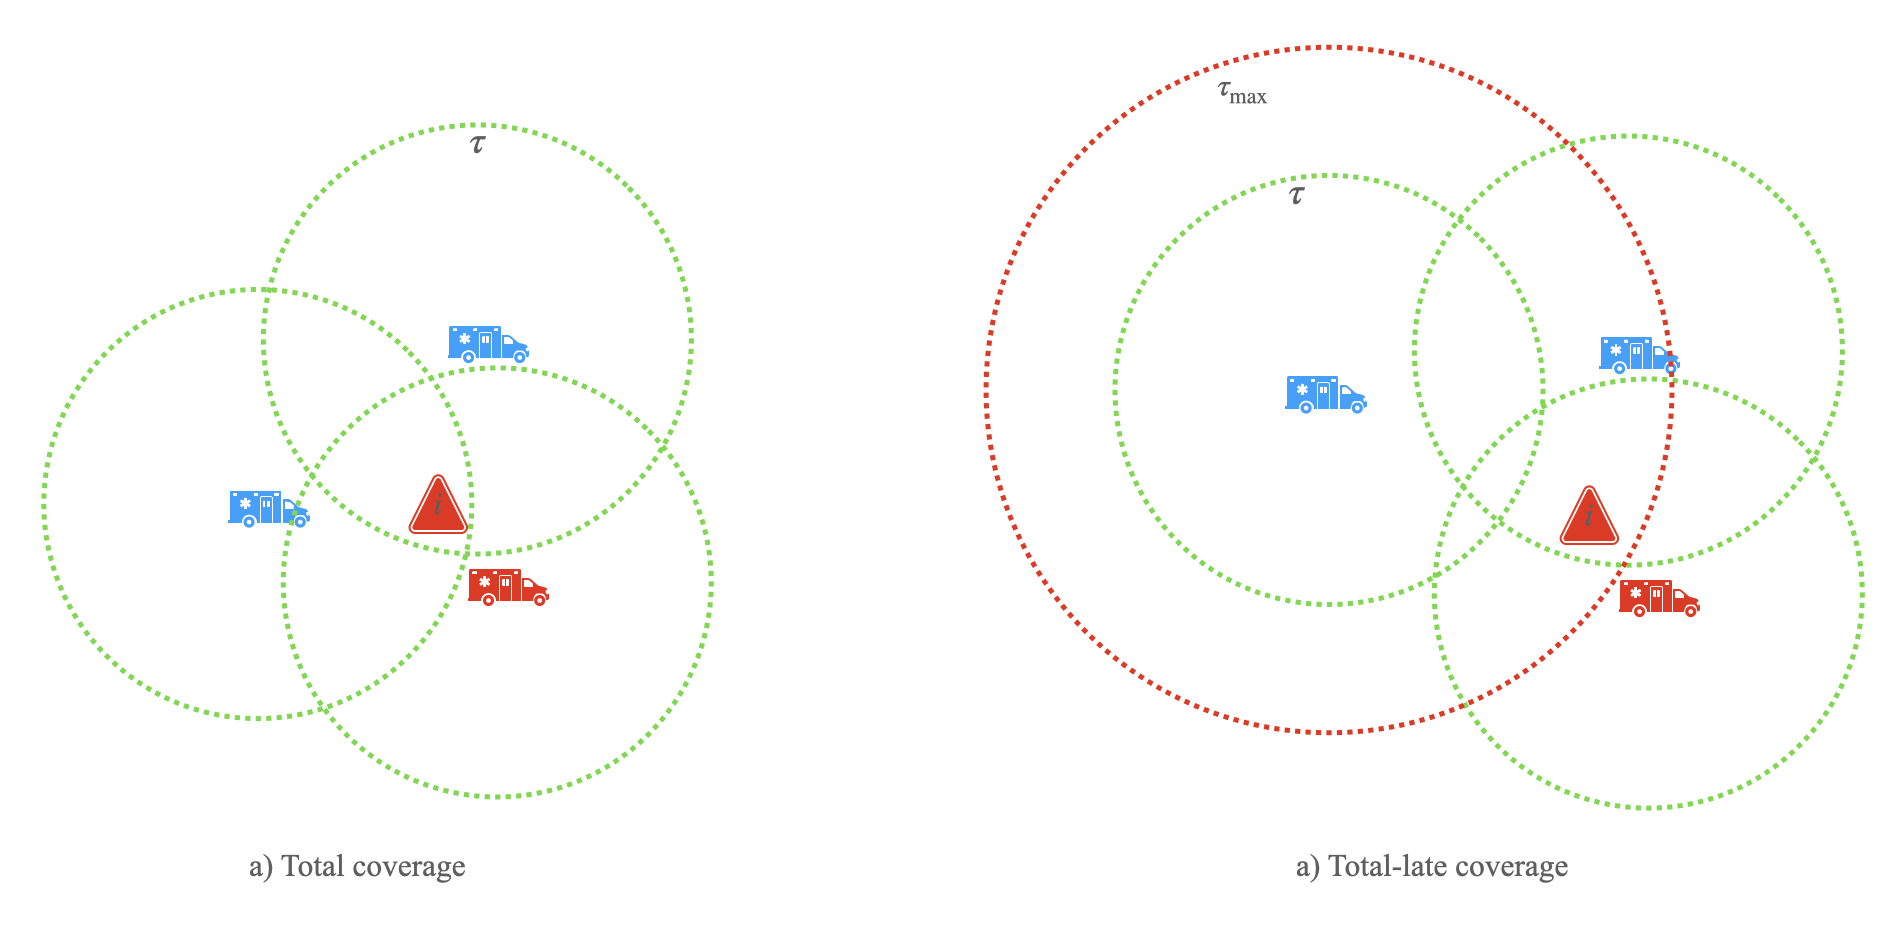
\includegraphics[width=0.97\textwidth]{figures/IntroTotalCoverage.png}
    \caption{Two different coverage cases for a scenario $s\in S$ where $i\in I^s$ requires $a_{1i}^s=2$ basic ambulances (blue) and $a_{2i}^s=1$ advanced ones (red). Total coverage in the left: all ambulances arrive in less than the ideal time $\tau$. Total-late coverage in the right: at least one of the ambulances arrives between $ (\tau,\tau_{\max})$.}
    \label{coverage-types}
\end{figure}

Figure~\ref{coverage-types} illustrates two different coverage cases for a scenario $s\in S$ where $i\in I^s$ requires $a_{1i}^s=2$ basic ambulances (indicated in blue) and $a_{2i}^s=1$ advanced one (indicated in red). All ambulances arrive in less than the ideal time $\tau$ for the Total coverage (left-hand-side figure). In the Total-late coverage line, at least one of the ambulances is late since it arrives between $ (\tau,\tau_{\max})$ (right-hand-side figure). In the Partial coverage, the number of required ambulances is not met, but at least they arrive in less than the ideal time $\tau$. In the Partial-late coverage, not only are there not enough ambulances to cover the demand point, but they arrive late, that is, between $ (\tau,\tau_{\max})$. In the Null coverage, ambulances may be dispatched to the demand point, but since the arrival times are larger than $\tau_{\max}$, the demand point is considered uncovered. 


Table~\ref{general_parameters} summarizes the sets and parameters used to describe the EVCP problem.
\begin{table}[htb]
\centering
\begin{tabular}{ll}
%\hline
%\multicolumn{2}{c}{Sets and parameters for the EVCP problem}   \\ 
\hline
$I$      & set of possible demand points (possible accident places)   \\
$L$          & set of possible ambulance location sites                         \\
$K$          & set of ambulance types                         \\
$\eta_k$    & total number of ambulances in the system of type $k \in K$                  \\
$r_{li}$ & response time from potential site $l \in L$ to demand point $i \in I$       \\
$\tau$       &    ideal response time to give the patients the first medical aid in \\ & an emergency                                  \\
$\tau_{max}$ &     maximum response time to cover an accident                                           \\ 
$c_{li}$ & benefit from traveling from potential site $l \in L$ to demand \\ & point $i \in I$   \\
\hline
$S$      & set of scenarios \\
$a_{ki}^s$ & number of needed ambulances of type $k \in K$ at demand \\ & point $ i \in I, s \in S$                          \\
$I^s$         &   set of demand points for $s\in S$ with at least a value \\ & $a_{ki}^s \neq 0$ for $ i \in I, k\in K$  \\
\hline
\end{tabular}
\caption{Sets and parameters to describe the EVCP problem.}
\label{general_parameters}
\end{table}

 


\section{Maximum Expected Coverage stochastic formulation for the EVCP problem}\label{sec:Modelo1}


%%%%%%%%%%%%%%%%%%%%%%
%%%%%%%%%%%%%%%%%%%%%%
%%% FIRST MODEL
%%%%%%%%%%%%%%%%%%%%%%
%%%%%%%%%%%%%%%%%%%%%

The Maximum Expected Coverage (MEC) formulation is a stochastic integer quadratic programming model in which the first stage variables $x_{lk}$ correspond to the number of ambulances of type $k\in K$ located at $l\in L$,
and the second-stage variables correspond
to the ambulance dispatching decisions at each demand point for each scenario $s \in S$: % $x_{lk} $ is the number of ambulances of type $k  \in K$  located at potential site $l \in L$. Also,
 \begin{equation*}
       y^s_{lki} = \left\{
       \begin{array}{ll} 
        1 & \text{if an ambulance of type } k\in K \text{ in location } l\in L \\
        & \text{ is dispatched to demand point }i\in I^s, \text{ for scenario }  s\in S, \\
        0 & \text{otherwise}.
       \end{array} \right.
\end{equation*}
%We consider that all scenarios have the same probability of occurrence. DECIR QUE ES UN MUESTREO.
%Each active demand point is considered a whole event, contrary to the disaggregated model presented in Section~\ref{Modelo2}. So, 
We defined the following binary variables related to the \textit{total} and \textit{total-late} coverages related to the response times of the ambulances to the demand point $i\in I^s, s\in S$:
\begin{equation*}
       f^s_{i} = \left\{
       \begin{array}{ll} 
        1 & \text{if demand point  } i\in I^s \text{ has a \textit{total} coverage}, \\
         0 & \text{otherwise},
       \end{array} \right.
\end{equation*}
\begin{equation*}
       g^s_{i} = \left\{
       \begin{array}{ll} 
        1 & \text{if demand point  } i\in I^s \text{ has a \textit{total-late} coverage}, \\
         0 & \text{otherwise}.
       \end{array} \right.
\end{equation*}
The following sets of binary variables are for the \textit{partial} and \textit{partial-late} coverages of the ambulances to the emergencies:
\begin{equation*}
       h^s_{i} = \left\{
       \begin{array}{ll} 
        1 & \text{if demand point  } i\in I^s \text{ has a \textit{partial} coverage}, \\
         0 & \text{otherwise},
       \end{array} \right.
\end{equation*}
\begin{equation*}
       w^s_{i} = \left\{
       \begin{array}{ll} 
        1 & \text{if demand point  } i\in I^s \text{ has a \textit{partial-late} coverage}, \\
         0 & \text{otherwise}.
       \end{array} \right.
\end{equation*}
Finally, to indicate a null coverage of a demand point, we define
\begin{equation*}
       z^s_{i} = \left\{
       \begin{array}{ll} 
        1 & \text{if active demand point  } i\in I^s \text{ has a \textit{null} coverage}, \\
         0 & \text{otherwise}.
       \end{array} \right.
\end{equation*}


 
% MODEL

The MEC formulation is as follows.
\begin{equation}
    \max_{x} \mathbb{E}_{s\in S} [ \mathcal{Q}^s(x)]
    \label{eq1}
\end{equation}
where
\begin{equation}
    \mathcal{Q}^s(x) = %\max_{y^s, \alpha^s, \beta^s, \delta^s, \varphi^s, \gamma^s} 
    \sum_{i \in I^s}  (  \alpha_1 f_i^s + \alpha_2 g_i^s + \alpha_3 h_i^s + \alpha_4  w_i^s -\phi z_i^s ) \nonumber
    %\label{eq2}
\end{equation}
%subject to
\begin{align}
\text{ s.t. } & \sum_{l \in L} x_{lk} \leq \eta_k   &\quad&  k \in K
    \label{eq3}\\
   & \sum_{i\in I^s}y_{lki}^s \leq x_{lk}  &&  l \in L,   k \in K,  s \in S 
    \label{eq4}\\
 %       & \textcolor{magenta}{y_{l1i}^s \leq a_{i1}^s} && \textcolor{magenta}{i \in I, l \in L,  s \in S \label{eq5}\\
%    & \textcolor{magenta}{y_{l2i}^s \leq a_{ik}^s} && \textcolor{magenta}{i \in I, l \in L,   k \in K,  s \in S } \label{eq5_1}\\ 
     &    f_i^s\sum_{k \in K}a_{ki}^s   \leq \sum_{l \in L} \sum_{k \in K} c_{li} y_{lki}^s, \quad   a_{2i}^s f_i^s \leq \sum_{l \in L}   c_{li} y_{l2i}^s &&  i \in I^s,   s \in S \label{eq6}\\
     %&  a_{2i}^s f_i^s \leq \sum_{l \in L}   c_{li} y_{l2i}^s &&  i \in I^s,   s \in S \label{eq6}\\
   % & \sum_{k \in K } a_{ki}^s f_i^s \leq \sum_{l \in L} \sum_{k \in K} c_{li} y_{lki}^s &&  i \in I^s,   s \in S \label{eq6}\\
%\end{alignat}
%\begin{align}
     &   g_i^s  \sum_{k \in K}  a_{ki}^s \leq \sum_{l \in L} \sum_{k \in K} y_{lki}^s, \quad   a_{2i}^s g_i^s \leq \sum_{l \in L}   y_{l2i}^s &&   i \in I^s, s \in S \label{eq7}\\
    & g_i^s \leq M \left( \sum_{l \in L} \sum_{k \in K } y_{lki}^s - \sum_{l \in L} \sum_{k \in K} c_{li} y_{lki}^s \right) &&  i \in I^s,   s\in S   \label{eq8}\\
  %Parcial  
  &  h_i^s \leq   \sum_{k \in K}  a_{ki}^s - \sum_{l \in L} \sum_{k \in K} y_{lki}^s, \quad  h_i^s \leq   a_{2i}^s - \sum_{l \in L}   y_{l2i}^s  && i \in I^s,    s\in S
    \label{eq9}\\
 %Parcial 
 & \sum_{l \in L} \sum_{k \in K} y_{lki}^s h_i^s \leq \sum_{l \in L} \sum_{k \in K} c_{li} y_{lki}^s && i \in I^s,  s\in S
    \label{eq10}
     \end{align}
\begin{align}
   %P-late 
   &  w_i^s \leq  \sum_{k\in K}a_{ki}^s - \sum_{l \in L} \sum_{k \in K} y_{lki}^s, \quad  w_i^s \leq   a_{2i}^s - \sum_{l \in L}   y_{l2i}^s &&  i \in I^s,  s\in S
    \label{eq11}\\
   & w_i^s \leq M \left( \sum_{l \in L} \sum_{k \in K} y_{lki}^s - \sum_{l \in L} \sum_{k \in K} c_{li} y_{lki}^s \right)  && i \in I^s,  s\in S 
    \label{eq12}\\
  %Null 
  & \sum_{l \in L} \sum_{k \in K} y_{lki}^s + z_i^s \geq 1 && i \in I^s,   s \in S  \label{eq13}\\
    & f_i^s + g_i^s + h_i^s + w_i^s + z_i^s = 1  && i \in I^s,  s \in S 
    \label{eq14}\\
  &  x_{lk} \in \mathbb{Z}^+ , y_{lki}^s \in \{ 0,1 \} && l \in L,   k \in K, i \in I^s, s \in S
    \label{eq15}\\
    & f_i^s, g_i^s, h_i^s, w_i^s, z_i^s \in \{ 0,1 \}  && i \in I^s,   s \in S.
    \label{eq16}
\end{align}

The objective function (\ref{eq1}) maximizes the expected value of the weighted coverage of the emergencies. %The last term is a penalty for uncovered demand points.
%Vector $x$ contains all the variables $x_{lk} \in \mathbb{Z}^+$ for $l \in L,   k \in K$. 
The parameters $\alpha_1 , \alpha_2, \alpha_3$ and $\alpha_4$ are normalized weights that ponder the coverage type, and $\phi$ is the penalty for the null coverage. We assume that every scenario is equally probable since each $s\in S$ represents a sample of the high-demand period we are interested in.

Constraints (\ref{eq3}) establish the available number of ambulances per type.
Constraints (\ref{eq4}) establish the relationship between the first and second-stage variables, meaning no ambulances can be dispatched from a potential site if no ambulances are located there.
The \textit{total} coverage of an emergency is defined by constraints (\ref{eq6}). Indeed, if the time response of the location of the ambulances to the emergency is less than $\tau$, then all $c_{li}=1$ and total coverage variables $f_i^s$ can be equal to one, for $l\in L, i\in I^s, s\in S$. The \textit{total-late} coverage is defined by constraints (\ref{eq7}) and (\ref{eq8}). Constraints (\ref{eq7}) allow the total-late coverage variables $g_i^s$ to be one when dispatching variables are active. Meanwhile, constraints (\ref{eq8}) track the demand points where the response time is between $(\tau,\tau_{\max})$ when the difference in the right-hand side of the equation is positive, that is, when there is a value $c_{lj}<1$ associated to a dispatched ambulance, for $l\in L, i\in I^s, s\in S$. Note that this difference may be decimal, so we include a big $M$ value. The \textit{partial} coverage is defined by constraints (\ref{eq9}) and (\ref{eq10}). Recall that, in this case, not all the needed ambulances are dispatched to the emergencies, but the ones that are dispatched have an ideal response time. Thus, constraints (\ref{eq9}) activate variables $h_i^s$ if the number of dispatched ambulances is less than the required ones. Quadratic constraints (\ref{eq10}) guarantee that the dispatched ambulances arrive within the ideal response time, that is, their corresponding value $c_{li}=1$, for $l\in L, i\in I^s, s\in S$. Constraints (\ref{eq11}) and (\ref{eq12}) define the \textit{partial-late} coverage. Constraints (\ref{eq11}) activate the $w_i^s$ variables when the number of required ambulances exceeds the number of dispatched ones. Similarly to the total-late coverage, constraints (\ref{eq12}) track the ambulances with a response time larger than the ideal one and must be multiplied by a big $M$. The \textit{null} coverage is activated by constraints (\ref{eq13}). All the coverage constraints are related to constraint (\ref{eq14}) that ensures only one type of coverage for each emergency. Finally, (\ref{eq15}) and (\ref{eq16}) establish the nature of the decision variables. 

The novelty of the MEC model is the stochastic total/partial coverage per emergency by two types of ambulances. Nevertheless, the related number of variables and constraints is usually large. Moreover, constraints (\ref{eq10}) are quadratic. An integer linear stochastic model with a classical linearization method could be easily formulated. Still, previous experiments showed similar times between the linearized and the quadratically constrained models when solved with integer programming solvers, so we keep the quadratic one for the Intelligent Feedback methodology presented in the next section.


\section{Surrogate-based feedback method for the EVCP problem} \label{IF}


The EVCP problem is $\mathcal{NP}$-hard since the classical $\mathcal{NP}$-hard facility location problem \citep{megiddo1982complexity} could be polynomially reduced to it. The MEC model is experimentally challenging to solve, even for medium-sized instances, as shown in Section~\ref{Exp}. Thus, we propose a surrogate-based feedback method (SBFM) to obtain approximate solutions to the EVCP problem based on an auxiliary disaggregated model, named \textit{Surrogate Ambulance-Based Coverage} (SABC) model, which is faster to solve. 

The SABC model's essential characteristic is that its objective function does not rely on emergency coverage, as in the MEC model; it only counts the number of ambulances sent on time, late, or null to emergency demand points. Moreover, its resolution time is extremely fast since it requires fewer variables and constraints than the MEC model. However, disaggregating an emergency situation into the number of ambulances needed does not capture emergency coverage, which is crucial for an EMS system.

In addition to the location variables $x_{li}$, the SABC model requires the following ambulance dispatching binary variables for $k\in K, l\in L, i\in I^s, s\in~S$: 
\begin{alignat}{2}
       u^s_{lki} & = \left\{
       \begin{array}{ll} 
        1 & \text{if ambulance of type $k$ is dispatched from site $l$ 
             to point $i$} \\
          &   \text{with response time less than $\tau$},\\
         0 & \text{otherwise},
       \end{array} \right.\nonumber\\
%
       v^s_{lki} & = \left\{
       \begin{array}{ll} 
        1 & \text{if ambulance of type $k$ is dispatched from site $l$ 
             to $i$ }\\
             &   \text{with response time in $(\tau,\tau_{\max})$},\\
         0 & \text{otherwise}.
       \end{array} \right.\nonumber
\end{alignat}
Variables $u^s_{lki}$ indicate the ambulances with an ideal response time dispatched from the location sites corresponding to a decay function value $c_{li}=1$. While variables $v^s_{lki}$ indicate the ones with a larger than $\tau$ response time which have a value $c_{li} < 1$. The number of required ambulances $k$ in an emergency demand point $i$ that are not dispatched are counted by integer variable $\zeta^s_{ki}$, for  $k\in K, i\in I^s, s \in S$. The SABC is as follows. 
\begin{align}
      \max_{x} \ \ & \mathbb{E}_s [ \mathcal{G}^s(x)],
    \label{eq18}\\
 \text{ where } &  \mathcal{G}^s(x) =  \left[ {\sum_{l \in L} \sum_{k \in K} \sum_{i \in I^s}} (\beta_1 u_{lki}^s + \beta_2 v_{lki}^s) - \sum_{k \in K} \sum_{i \in I^s}  \phi \zeta_{ki}^s \right]
    \label{obj19}
\end{align}
\begin{align}
\text{s.t. }  &  \sum_{l \in L} x_{lk} \leq \eta_k  && k \in K \label{eq20}  
  \\
  &    \sum_{i\in I^s}(u_{lki}^s + v_{lki}^s) \leq x_{lk} &&   l \in L,   k \in K,  s \in S  
   \label{eq21}  \\  
  &  u_{lki}^s \leq c_{li}  && l \in L,  i \in I^s,   k \in K,  s \in S    \label{eq22}\\
  &  u_{lki}^s + v_{lki}^s \leq 1 && l \in L,    i \in I^s,   k \in K,   s \in S
    \label{eq23}\\
    &  a_{1i}^s +a_{2i}^s = \sum_{l \in L}\sum_{k \in K}( u_{lki}^s + v_{lki}^s + \zeta_{ki}^s )  && i \in I^s, s \in S
    \label{eq24}\\
    &   a_{2i}^s  \leq  \sum_{l \in L}( u_{l2i}^s + v_{l2i}^s  + \zeta_{2i}^s ) &&  i \in I^s, s \in S
    \label{eq24bis}\\
%     & \textcolor{red}{NOVAN\sum_{k\in K}  u_{lki}^s \leq  a_{i1}^s , \quad   \sum_{l\in L}(u_{l2i}^s +v_{l2i}^s)\leq \sum_{k\in K}a_{ik}^s } &&  i \in I, l \in L,  s \in S \label{ALS1}\\
    %& \textcolor{magenta}{} & \textcolor{magenta}{i \in I, l \in L,   k \in K,  s \in S }\label{eq25_1}\\
%    & \textcolor{red}{NOVAN}\sum_{k\in K} v_{lki}^s \leq a_{i1}^s, \quad v_{l2i}^s \leq a_{i2}^s  &&  i \in I, l \in L,  s \in S    \label{ALS2}\\
    %& \textcolor{magenta}{v_{l2i}^s \leq a_{ik}^s} & \textcolor{magenta}{i \in I, l \in L,   k \in K,  s \in S }\label{eq26_1}\\ 
%   & \sum_{l\in L} (u_{lki}^s + v_{lki}^s) \leq a_{ki}^s  &  i \in I^s,   k \in K,   s \in S    \label{eq25}\\
   & x_{lk}, \zeta_{ki}^s \in \mathbb{Z}^+, u_{lki}^s, v_{lki}^s \in \{ 0,1 \}  && l \in L,   k \in K, i \in I^s, s \in S      \nonumber
\end{align}

The objective function \eqref{eq18} maximizes the expected value of the on-time and late dispatched ambulances minus a penalty $\phi$ for the required ambulances that could not be dispatched in less than $\tau_{\max}$ time response. The weights $\beta_1 > \beta_2$ are normalized parameters that prioritize the ambulances dispatched with a response time less than $\tau$. As in the previous model, no more than the available ambulances can be located on the sites, corresponding to constraints \eqref{eq20}. The number of ambulances dispatched on time or late is less than the number of ambulances located, as indicated by constraints \eqref{eq21}. Constraints (\ref{eq22}) define the ambulances dispatched with an ideal response time of less than $\tau$. Thus, if $c_{li}=1$, then the ambulance will have an ideal response time, while constraints (\ref{eq23}) activate the late variables for which their response time is between $(\tau, \tau_{\max})$. With constraints (\ref{eq24}) and (\ref{eq24bis}), the non-covered emergencies, $\zeta_{ki}^s$ variables are defined for $i \in I^s, s \in S$. Recall that advanced ambulances can be dispatched instead of basic ones. %, we add restrictions \eqref{ALS1} and \eqref{ALS2}. 
Finally, the nature of the variables is stated. 


\textit{The surrogate-based feedback method:} Under the SBFM,
the SABC stochastic model is solved first.
From its optimal solution, we obtain the location of the ambulances of the first stage corresponding to the value of $x_{lk}$ variables, for $l\in L, k \in K$. Let the solution vector of these values be called $x^\text{SABC}$. 
Then, in the allocation stage, we solve MEC 
taking $x^\text{SABC}$ as input. We call this
model MEC($x^\text{SABC}$), or simply MEC(SABC), implying
that it is the solution of the MEC model with the location variables fixed with the solution of the surrogate model SABC.
Since the first stage variables are fixed, the MEC(SABC) model becomes easier to solve and yields high-quality solutions. We could implement a local search neighborhood based on the location variables $x_{lj}$ to diversify the solution yield by variables $x^\text{SABC}$. However, experimental results show that the quality of the SBFM solutions is exceptionally high with a single feedback.  

As mentioned, the SABC auxiliary model is a surrogate for the MEC formulation. Thus, the solutions obtained by the MEC and SABC are not equivalent. Nevertheless, the solutions of the SABC model can be mapped into solutions for the EVCP problem, as shown in Algorithm \ref{alg:cap}. In this manner, we can compare both models regarding emergency coverage, even if the SABC model is short-sighted regarding this objective. 
Step 3 activates the total coverage when all the required ambulances arrive in less than $\tau$ response time. Step 4 verifies if a dispatched ambulance has a response time in $(\tau,\tau_{\max})$, corresponding to the total-late coverage. Step 6 checks that not all the required ambulances are dispatched but they arrive between the ideal time, while Step 8 verifies that the dispatched ambulances are not all the required ones and at least one of them has a response time in $(\tau,\tau_{\max})$. Finally, Step 10 activates the null variable.


\begin{comment}
\section{Intelligent Feedback methodology for the EVCP problem} \label{IF}

The MEC model is experimentally hard to solve, even for medium-size instances, as shown in Section~\ref{cap:Exp}. Thus, we propose the  Intelligent Feedback methodology to obtain approximate solutions for the EVCP problem based on an auxiliary disaggregated model, named \textit{Surrogate Ambulance-Based Coverage} (SABC) model. 

In addition to the location variables $x_{li}$, the SABC model requires the following binary ambulance dispatching variables for $k\in K, l\in L, i\in I^s, s\in~S$: 
\begin{equation*}
       u^s_{lki} = \left\{
       \begin{array}{ll} 
        1 & \text{if ambulance of type $k$ is dispatched from site $l$ 
             to point $i$} \\
          &   \text{ with response time less than $\tau$},\\
         0 & \text{otherwise},
       \end{array} \right.
\end{equation*}
\begin{equation*}
       v^s_{lki} = \left\{
       \begin{array}{ll} 
        1 & \text{if ambulance of type $k$ is dispatched from site $l$ 
             to $i$ }\\
             &   \text{ with response time in $(\tau,\tau_{\max})$},\\
         0 & \text{otherwise}.
       \end{array} \right.
\end{equation*}
Variables $u^s_{lki}$ indicate the ambulances with an ideal response time dispatched from the location sites corresponding to a decay function value $c_{li}=1$. While variables $v^s_{lki}$ indicate the ones with a larger than $\tau$ response time which have a value $c_{li} < 1$. The number of required ambulances $k$ in an emergency demand point $i$ that are not dispatched are counted by integer variable $\zeta^s_{ki}$, for  $k\in K, i\in I^s, s \in S$. The SABC is as follows. 
\begin{equation}
      \max_{x} \mathbb{E}_s [ \mathcal{G}^s(x)]
    \label{eq18}
\end{equation}
where 
\begin{equation*}
    \mathcal{G}^s(x) =  \left[ {\sum_{l \in L} \sum_{k \in K} \sum_{i \in I^s}} (\beta_1 u_{lki}^s + \beta_2 v_{lki}^s) - \sum_{k \in K} \sum_{i \in I^s}  \phi \zeta_{ki}^s \right]
    \label{obj19}
\end{equation*}
subject to
\begin{align}
  &  \sum_{l \in L} x_{lk} \leq \eta_k  & k \in K \label{eq20}  
  \\
  &    \sum_{i\in I^s}(u_{lki}^s + v_{lki}^s) \leq x_{lk} &   l \in L,   k \in K,  s \in S  
   \label{eq21}  \\  
  &  u_{lki}^s \leq c_{li}  & l \in L,  i \in I^s,   k \in K,  s \in S    \label{eq22}\\
  &  u_{lki}^s + v_{lki}^s \leq 1 & l \in L,    i \in I^s,   k \in K,   s \in S
    \label{eq23}\\
    & a_{1i}^s = \sum_{l \in L}\sum_{k \in K}( u_{lki}^s + v_{lki}^s + \zeta_{ki}^s )  & i \in I^s, s \in S
    \label{eq24}\\
    &   a_{2i}^s = \sum_{l \in L}( u_{l2i}^s + v_{l2i}^s + \zeta_{2i}^s )  & i \in I^s, s \in S
    \label{eq24bis}\\
     & \sum_{k\in K}  u_{lki}^s \leq  a_{i1}^s , \quad u_{l2i}^s \leq a_{i2}^s &  i \in I, l \in L,  s \in S
    \label{ALS1}\\
    %& \textcolor{magenta}{} & \textcolor{magenta}{i \in I, l \in L,   k \in K,  s \in S }\label{eq25_1}\\
    & \sum_{k\in K} v_{lki}^s \leq a_{i1}^s, \quad v_{l2i}^s \leq a_{i2}^s  &  i \in I, l \in L,  s \in S
    \label{ALS2}\\
    %& \textcolor{magenta}{v_{l2i}^s \leq a_{ik}^s} & \textcolor{magenta}{i \in I, l \in L,   k \in K,  s \in S }\label{eq26_1}\\ 
%   & \sum_{l\in L} (u_{lki}^s + v_{lki}^s) \leq a_{ki}^s  &  i \in I^s,   k \in K,   s \in S    \label{eq25}\\
   & x_{lk}, \zeta_{ki}^s \in \mathbb{Z}^+, u_{lki}^s, v_{lki}^s \in \{ 0,1 \}  & l \in L,   k \in K, i \in I^s, s \in S      \nonumber
\end{align}

The objective function \eqref{eq18} maximizes the expected value of the on-time and late dispatched ambulances minus a penalty $\phi$ for the required ambulances that could not be dispatched in less than $\tau_{\max}$ time response. Weights $\beta_1 > \beta_2$ are normalized parameters prioritizing the dispatched ambulances with a response time less than $\tau$. As in the previous model, no more than the available ambulances can be located in the sites, corresponding to constraints \eqref{eq20}. The number of on-time or late dispatched ambulances is less than the number of located ambulances, as indicated by constraints \eqref{eq21}. Constraints (\ref{eq22}) define the dispatched ambulances with an ideal response time of less than $\tau$. Thus, if $c_{li}=1$, then the ambulance will have an ideal response time, while constraints (\ref{eq23}) activate the late variables for which their response time is between $(\tau, \tau_{\max})$. With constraints (\ref{eq24}) and (\ref{eq24bis}), the non-covered emergencies, $\zeta_{ki}^s$ variables, are defined, for $i \in I^s, s \in S$.  Recall that advanced ambulances can be dispatched instead of basic ones. %, we add restrictions \eqref{ALS1} and \eqref{ALS2}. 
Finally, the nature of the variables is stated.
 
The key characteristic of the SABC model is that the objective function does not rely on emergency coverage as in the MEC model; it only counts the number of on-time, late, or null ambulances sent to the emergency demand points. Moreover, its resolution time is extremely fast since it requires fewer variables and constraints than the MEC one. Nevertheless, disaggregating an emergency situation into the number of required ambulances does not capture emergency coverage, which is crucial for an EMS system.

\textit{The surrogate-based feedback method:} Under the SBFM,
the SABC stochastic model is solved first.
From its optimal solution, we obtain the location of the ambulances of the first stage corresponding to the value of $x_{lk}$ variables, for $l\in L, k \in K$. Let the solution vector of these values be called $x^\text{SABC}$. 
Then, in the allocation stage, we solve MEC 
taking $x^\text{SABC}$ as input. We call this
model MEC($x^\text{SABC}$), or simply MEC(SABC), implying
that it is the solution of the MEC model with the location variables fixed with the solution of the surrogate model SABC.
Since the first stage variables are fixed, the MEC(SABC) model becomes easier to solve and yields high-quality solutions. We could implement a local search neighborhood based on the location variables $x_{lj}$ to diversify the solution yield by variables $x^\text{SABC}$. However, experimental results show that the quality of the SBFM solutions is exceptionally high with a single feedback.  

%In the Intelligent Feedback methodology for the EVCP problem, we first solve the SABC stochastic model.  From this optimal solution, we obtain the location of the ambulances of the first stage corresponding to the value of $x_{lk}$ variables, for $l\in L , k \in K$. We use these values as input to the MEC model.
%Since the first stage variables are fixed, the MEC(SABC) becomes easier to solve and yields high-quality solutions. To diversify the solution, we could implement a local search neighborhood based on the location variables $x_{lj}$. Nevertheless, experimental results show that the quality of the solutions using the MEC(SABC) methodology is extremely high with a single feedback.    

As mentioned, the SABC auxiliary model is a surrogate for the MEC formulation. Thus, the solutions obtained by the MEC and SABC are not equivalent. Nevertheless, the solutions of the SABC model can be mapped into solutions for the EVCP problem, as shown in Algorithm \ref{alg:cap}. In this manner, we can compare both models regarding emergency coverage, even if the SABC model is short-sighted regarding this objective. 
Step 3 activates the total coverage when all the required ambulances arrive in less than $\tau$ response time. Step 4 verifies if a dispatched ambulance has a response time in $(\tau,\tau_{\max})$, corresponding to the total-late coverage. Step 6 checks that not all the required ambulances are dispatched but they arrive between the ideal time, while Step 8 verifies that the dispatched ambulances are not all the required ones and at least one of them has a response time in $(\tau,\tau_{\max})$. Finally, Step 10 activates the null variable.
\end{comment}

 
\begin{algorithm}
\caption{Transformation of a SABC solution into a MEC solution }\label{alg:cap}
\begin{algorithmic}[1]
\State \textbf{require} solution of the SABC model $(\bar{x},\bar{u},\bar{v})$
\For{ $i\in I^s, s\in S$}
    \State \textbf{if } $\sum_{l\in L,k\in K} \bar{u}^s_{lki}= a^s_{ki}$ \textbf{then}  $f^s_i=1$ \Comment{total coverage}
    \State \textbf{if} $\sum_{l\in L,k\in K} \bar{u}^s_{lki}  < a^s_{ki}$ and $ \sum_{l\in L,k\in K} \bar{u}^s_{lki} +\bar{v}^s_{lki} = a^s_{ki}$ 
    \State $\quad $ \textbf{then} $g^s_i=1$ \Comment{total-late coverage}
    \State \textbf{if } $ \sum_{l\in L,k\in K} \bar{u}^s_{lki}  < a^s_{ki}$ and $\sum_{l\in L,k\in K}\bar{v}^s_{lki}=0$ 
    \State $\quad $ \textbf{then} $h^s_i=1$ \Comment{partial coverage}
    \State \textbf{if} $ \sum_{l\in L,k\in K} \bar{u}^s_{lki} +\bar{v}^s_{lki} < a^s_{ki}$ and $\sum_{l\in L,k\in K}\bar{v}^s_{lki}>0$ 
    \State $\quad $ \textbf{then} $w^s_i=1$ \Comment{partial-late coverage}
    \State \textbf{otherwise} $z^s_i=1$ \Comment{null coverage}
\EndFor
\State{ \textbf{return} MEC solution $(\bar{x},f,g,h,w, z)$   }
\end{algorithmic}
\end{algorithm}


\section{Matheuristic to improve the MEC model}
The Surrogate-based feedback method for the MEC(SABC) model has good results. However, a disadvantage of this method is that we obtain only one solution for the ambulance location from the surrogate model SABC. This is a problem because we disown the optimal solution for the MEC model and we are not sure if the SABC solution is close to that optimality. Trying to improve the solution $x^{SABC}$ we proposed a local search procedure, which is a matheuristic considering four neighborhoods, named as SABC Matheuristic. These four different neighborhoods are as follows:
\begin{itemize}
 \item Neighborhood 1, $(N_1)$: exchange one active potential site with another active potential site.
\item Neighborhood 2, $(N_2)$: pick half of an active potential site and add it to a non-active potential site.
\item Neighborhood 3, $(N_3)$: pick half of an active potential site and add it to another active potential site.
\item Neighborhood 4, $(N_4)$: exchange one active potential site with one non-active potential site.
\end{itemize}

$N_1$ and $N_4$ change BLS ambulances with BLS ambulances and then ALS ambulances with ALS ambulances. $N_2$ and $N_3$ change only BLS ambulances with BLS ambulances due to the small quantity of ALS ambulances in the EMS system.

The algorithm to solve the SABC Matheuristic has the $x^{SABC}$ as an initial solution. First, we obtain the value of the objective function for this initial solution, defined as $t^{SABC}$, which is the best solution at this point. Then, we construct the first neighborhood from the $x^{SABC}$. The $t^{SABC}$ objective value is compared with each neighbor's objective value, obtained as the MEC(SABC) methodology. If a neighbor's solution is better than $t^{SABC}$, we consider this solution as the best one for the Matheuristic and we save the objective value and variables results. Otherwise, we have the initial solution as the best one when the algorithm is finished. Regardless new best solution is the initial solution or not, we construct the second neighborhood from the $x^{SABC}$, and each neighbor is compared with the best solution at the moment. We repeat this procedure for the other two neighborhoods and, when the comparisons are finished, we obtain the best solution, as we can see at the Algorithm \ref{alg:cap_1}.

This procedure calculates each neighbor's objective value as in the MEC(SABC) methodology in the four different neighborhoods, which makes the SABC Matheuristic take so much time to check each neighborhood. This Matheuristic aids in improving $x^{SABC}$ solutions but not for all the instances, as we can see in Chapter \ref{cap:Exp}.


The next section compares the MEC, MEC(SABC), and even the SABC solutions.  



\begin{algorithm}
\caption{SABC Matheuristic to improve the MEC model}\label{alg:cap_1}
\begin{algorithmic}[1]
\State \textbf{require} solution of the SABC model $x^{SABC}$
\State $x^* = x^{SABC}$
\State $t^* = MEC(x^{SABC}) = t^{SABC}$
\While{not all neighborhoods $N_i$, where $i \in \{1,2,3,4\}$, have been visited}
	\For{$x' \in N_i$}
		\State Evaluate $t'=MEC(x')$ 
    	\State \textbf{if } $t' > t^*$ \textbf{then}  $x^* = x', t^*=t'$ 
    \EndFor
\EndWhile
\State{ \textbf{return} solution $(x^*,f,g,h,w,z)$ and objective value $t^*$ }
\end{algorithmic}
\end{algorithm}


%\chapter{Solution description}

\chapter{Experimental assessment}\label{cap:assess}

  This chapter presents an empirical assessment of models and the solution methodology previously described to solve the EVCP problem.  
We used Gurobi Optimizer 10.0.2 with Python 3.10 to solve the integer programming models MEC, SABC, and MEC(SABC).
The experiments were carried out on an Intel Core i7 at 3.1~GHz with 16~GB of RAM under the macOS Catalina 10.15.7 operating system. Each execution of the integer linear programming solvers had a CPU time limit of 10800 seconds. For SABC Matheuristic the solver had a CPU limit of 300 seconds for neighbor's evaluation and 10800 second in total.

\section{Instance generation} \label{instances}

The value ranges of our instance generator are based on real-world data taken from Monterrey, Mexico. In the literature, there are no suitable benchmarks for our problem. The databases for the Monterrey case study showed a larger number of possible demand points, $|I|\in \{168, 270, 500, 900, 1500\}$ compared to the one from the literature with $|I| \leq 270$ \citep{yoon2021stochastic}. The number of possible locations for ambulances in Monterrey is $|L|\in \{16,50,100\}$,  which is also larger than the one from the literature ($\leq$30) since not only hospitals and fire stations can be considered. We consider the whole city of Monterrey, so the number of ambulances $(\eta_1,\eta_2)= (35,20)$ is also greater than the ones from the literature cases (6 ambulances per type \citep{yoon2021stochastic}).
The number of scenarios is set to be as large as that in the literature $|S| \in \{10,50,100, 150, 200\}$. Thus, our benchmark has 15 instances for which five different scenario settings were built.
 
For each instance, we simulated a two-hour high-demand period. Each scenario $s\in S$ consists of a set of demand values per ambulance type and per demand point $\{a^s_{ki}\}_{k\in K, i\in I,s\in S}$.  
Fewer demand points imply a larger city grid and a larger proportion of emergencies per demand point. Therefore, when $|I|=168$, around 30\% of the demand points may have a value different from 0. In contrast, when $|I|=1500$, only 1\% of the demand points will require ambulances. This setting reflects the number of emergencies per hour observed in the case study. Instances are built such that most emergencies require a single ambulance, but as observed in real cases, some of them may require up to three ambulances. 
 
The ideal ambulance response time is $\tau = 10$ minutes, while the maximum response time is $\tau_{\max}=30$ minutes. For the MEC formulation, we use the following weights in the objective function~\eqref{eq1}: $\alpha_1= 0.65, \alpha_2= 0.2, \alpha_3= 0.1$, and $\alpha_4= 0.05$. In this manner, the total coverage is the most sought-after, while the partial-late cover has less benefit. Surprisingly, the value of the big $M$ of the model is not the main cause of the execution time of the MEC model. Thus, a simple value $M=1000$ is set. 

For the SABC objective function~\eqref{obj19} we use $\beta_1 = 0.7$ and $\beta_2 = 0.3$. These values reflect the aim to send primordially the required ambulances with an ideal response time. The penalty for null coverage in the MEC model or when a required ambulance cannot be dispatched to the emergency in less than $\tau_{\max}$ time in the SABC model is set to $\phi =   1/ |S|  + 0.0005$. 

All instances with their related scenarios and detailed solutions are available at \url{https://doi.org/10.6084/m9.figshare.25928401}.

%\section{Proposed solution}
%
%The methodology we will follow is:
%\begin{itemize}
%\item Do model construction to represent the thesis' problem proposed and an intelligent feedback formulation to obtain a similar location solution in less time. We will consider solutions from both formulations to decide which is the best to apply in a real case EMS system problem. The model will 
%\item Evaluate each one (model and intelligent feedback formulation) with a solver for small and medium instances. With these results, we can discuss if the formulations are well implemented or not according to the problem. We will use Gurobi Optimizer to program formulations' codes.
%\item Study stochastic programming in Julia, which is recently in the literature. We will see if Julia can solve our models, or we will study Branch and Benders cut solution used in a recent problem.
%\item Solve small and large-scale problems and evaluate the EMS system to know if we can improve patients' attention.
%\end{itemize}
%
%Our problem is focused on two decisions. The first is where to locate available ambulances within potential sites, and the second is how to dispatch them to accidents in scenarios. For these scenarios we have a sample set $S = \{s_1, s_2, ..., s_n\}$ taken from infinite scenarios possibles. Each scenario determines the number of ambulances type 1 and type 2 needed for each demand point. A scenario can be seen as follow:
%We will consider a demand point set $I = \{1, 2, 3, 4\}$. A possible scenario for these demand points will be $s_1 = \{(0, 1), (1, 2), (3, 0), (1, 1)\}$, which means that demand point $1$ needs zero type $1$ ambulances and one type $2$ ambulances, demand point $2$ needs one type $1$ ambulances and two type $2$ ambulances, and so on.
%
%Ambulance location is a fixed decision. Once the EMS system locates its ambulances at potential sites, these ambulances attend emergency calls and return to the potential sites where they were located. Considering this location, operators receiving emergency calls will have policies to determine what ambulance (or ambulances) is (are) best to attend an emergency at the demand call point. The mean idea for the EMS system's solution is to provide information about where to locate their ambulances depending on the number of ambulances needed at demand points in all scenarios.
%
%\subsection{Parameters} \label{instances}
%
%Our instance generator is based on real-world data taken from the city of Monterrey, Mexico. Table \ref{tab:yoon_p} compares our parameter settings with the ones used by of \cite{yoon2021stochastic}, a benchmark from the literature \textbf{for a similar problem??}.  
%
%\begin{table}[htb]
%    \centering
%    \begin{tabular}{ccc}
%    \hline
%       Parameters  &  Monterrey & Hannover, Mecklenburg \cite{yoon2021stochastic} \\
%       \hline
%       $|I|$  & $\{168, 270, 500, 900, 1500\}$ & \{168, 270\} \\
%        $|L|$  & $ \{16,50,100\}$ & \{16, 30\} \\
%        $(\eta_1,\eta_2)$ & $ (35,20) $ & $\{(3,3), (6,6)\}$\\
%       $|S|$   & $ \{10,50,100, 150, 200\}$  &   $ \{ 10, 50, 100, 150, 200\}$\\
%       \hline 
%    \end{tabular}
%    \caption{Comparison of instance size used for experimentation between our case study (Monterrey) and one form the literature.}
%    \label{tab:yoon_p}
%\end{table}
%The databases for the Monterrey case study showed a larger number of possible demand points $|I|$ compared to the one from the literature. The number of possible locations of the ambulances $|L|$ is also larger than the one from the literature since not only hospitals and fire stations can be considered. Since we consider the whole city of Monterrey, the number of ambulances $(\eta_1,\eta_2)$ is also larger than the ones from the literature cases. Finally, we noted that the number of scenarios could be as large as the ones from the literature. Thus, our benchmark has 15 instances for which five different scenario settings were built. The ideal ambulance response time is $\tau = 10$ minutes while the maximal response time is $\tau_{\max}=30$ minutes.  
%  
%For each instance, we simulated a two-hour high-demand period. Each scenario $s\in S$ consists of a set of demand values per type of ambulance and per demand point $\{a^s_{ki}\}_{k\in K, i\in I,s\in S}$. %\textcolor{magenta}{Each value $a_{ki}$ has a probability of being either null or positive depending on a Binomial distribution with probability $0 < N(0.5, 0.2)$, which is based on a Normal distribution. 
%%VALOR DE LA BINOMIAL * 500 Y LO TRUNCO A ENTEROSSuppose $\{a^s_{ki}\}_{k\in K, i\in I}$ is not zero. In that case, its value, which corresponds to the number of ambulances type $k$ at location $i$ in scenario $s$, is drawn from a sample function with probability taken by an Exponential distribution with $\lambda = \frac{d^s_i}{D}$ where $d_i$ is the sum of values $a_{ki}$ for each demand point $i \in I$, and $D$ is the total number of accidents for the $s \in S$ scenarios.}  
%Fewer demand points imply a larger grid of the city and a larger proportion of emergencies per demand point. Thus, when $|I|=168$, around 30\% of the demand points may have a value different from 0. On the contrary, when $|I|=1500$, only 1\% of the demand points will require ambulances. This setting reflects the number of emergencies per hour observed in the case study. The instances are built such that most emergencies require a single ambulance. 
% 
%  For the MEC formulation, we use the following weights in the objective function~\eqref{eq1}: $\alpha_1= 0.65, \alpha_2= 0.2, \alpha_3= 0.1$, and $\alpha_4= 0.05$. In this manner, the total coverage is the most sought one, while the partial-late cover is the one with less benefit. For the SABC objective function~\eqref{obj19} we use $\beta_1 = 0.7$ and $\beta_2 = 0.3$. These values reflect the aim to send primordially the required ambulances with an ideal response time. The penalty for null coverage in the MEC model or when a required ambulance cannot be dispatched to the emergency in less than $\tau_{\max}$ time in the SABC is set to $\phi =   1/ |S|  + 0.0005$.
%
%All the instances with their related scenarios are available at \textcolor{magenta}{FALTA figshare}.
%
%\section{Computing tools description}
%We used Gurobi Optimizer 10.0.2 with Python 3.10 to solve the integer programming models MEC, SABC, and MEC(SABC).
%The experiments were carried out on an Intel Core i7 at 3.1~GHz with 16~GB of RAM under the macOS Catalina 10.15.7 operating system. Each execution of the integer linear programming solvers has a CPU time limit of 10800 seconds. 
%
%%For large-scale problems, we will try the latest version of the Julia Programming Language for stochastic problems, which suggests some model decompositions into a master problem and a set of subproblems to solve stochastic models quickly and effectively \cite{biel2022efficient}. If these decompositions can not solve our problem, we will use a Branch and Benders cut to decompose our model, and we will code in Python.


\chapter{Experimental work}\label{cap:Exp}

%\begin{figure}[htb]
%    \centering
%    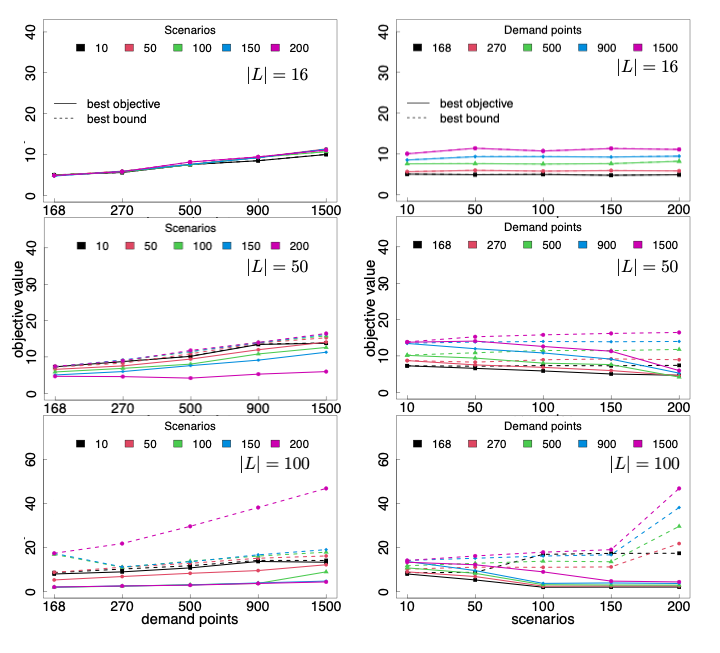
\includegraphics[width=.8\linewidth]{M1objectiveValue.png}
%    \caption{Best objective and the best bound of the objective function obtained by the MEC model concerning the demand points on the left side and the scenarios on the right side for different sizes of potential sites $|L|=\{16,50,100\}$. }
%    \label{fig:M1objV}
%\end{figure}

In this chapter, we analyze the parameters of the EVCP problem that impact the performance of the objective values of our stochastic methodologies. Several questions arise. We wish to investigate how sensitive the model is to the number of scenarios in terms of solution quality and solution time. We also want to determine the size of tractable instances.
%and to assess the impact in solution qualityDoes a high number of demand points imply a more challenging instance? Does the number of possible locations impact the efficiency of the models? 

\section{Objective values for the MEC, MEC(SABC) and SABC Matheuristic}

In this first experiment, we solve the instances using the original MEC model.
%RZand then using the SBFM.
% In this manner, we can evaluate the size of the instances for which MEC %can give optimal solutions and be able to compare this to the SBFM. 
 Figure~\ref{Obj_MEC} consists of six plots. The three plots in the left column vary the number of demand points (x-axis), comparing each one to the value of the objective function when different scenarios are tested. The three plots in the right-hand side column vary the tested number of scenarios and show the variation in the solution value for each number of demand points. The upper plots consider a number of possible locations for the ambulances of $|L|=16$, the middle plots of $|L|=50$, and the lower plots of $|L|=100$. Straight lines are the best objective values, while dotted ones are the best bounds found.

\begin{figure}[H]
\centering
\footnotesize
\stackunder[4pt]{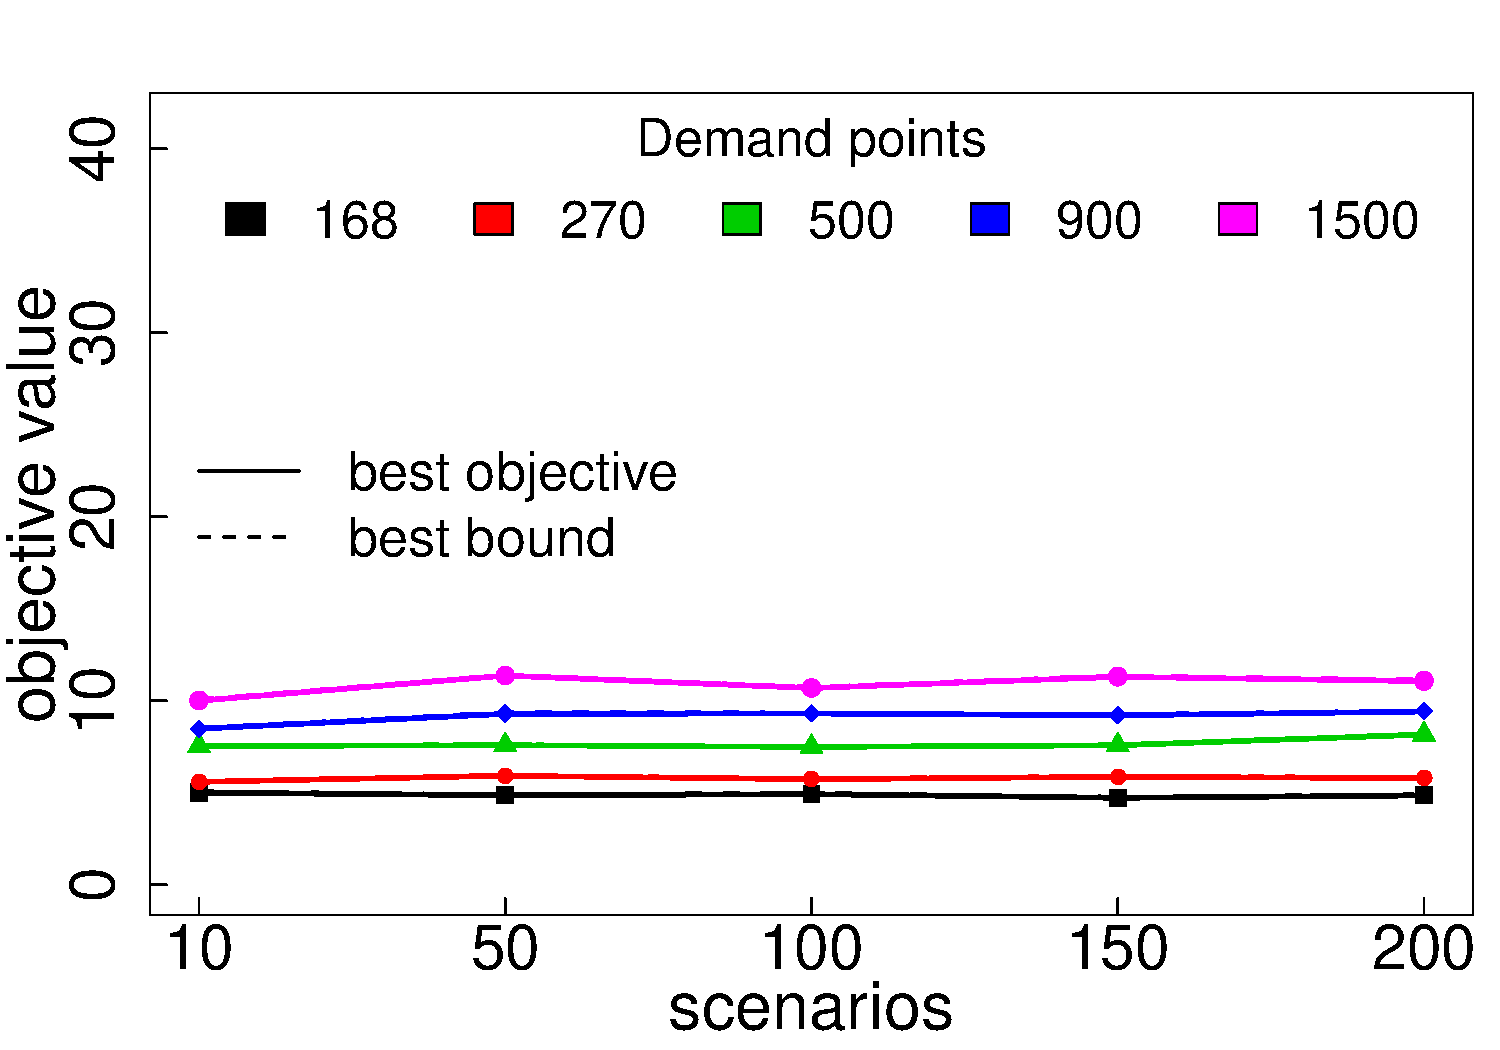
\includegraphics[width=0.42\textwidth]{Imagenes_Tesis/MEC/Obj_MEC_16.pdf}}{$|L|=16$}%
\hspace{0.4cm}%
\vspace{0.4cm}
\stackunder[4pt]{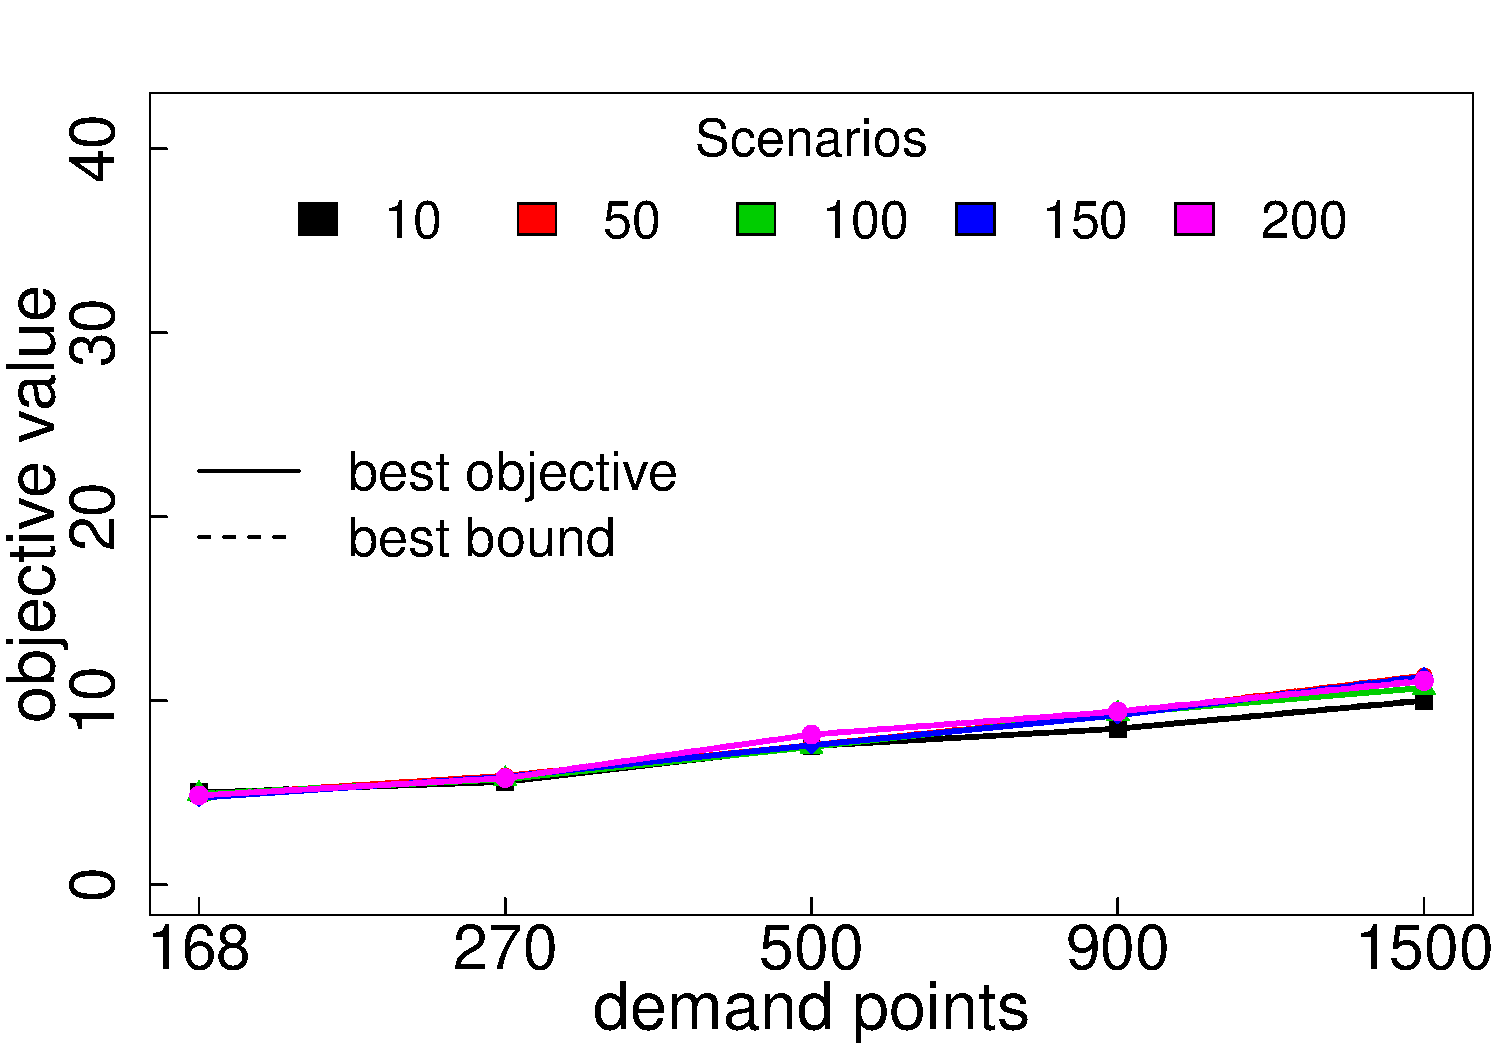
\includegraphics[width=0.42\textwidth]{Imagenes_Tesis/MEC/Obj_MEC_16_1.pdf}}{$|L|=16$}
\stackunder[4pt]{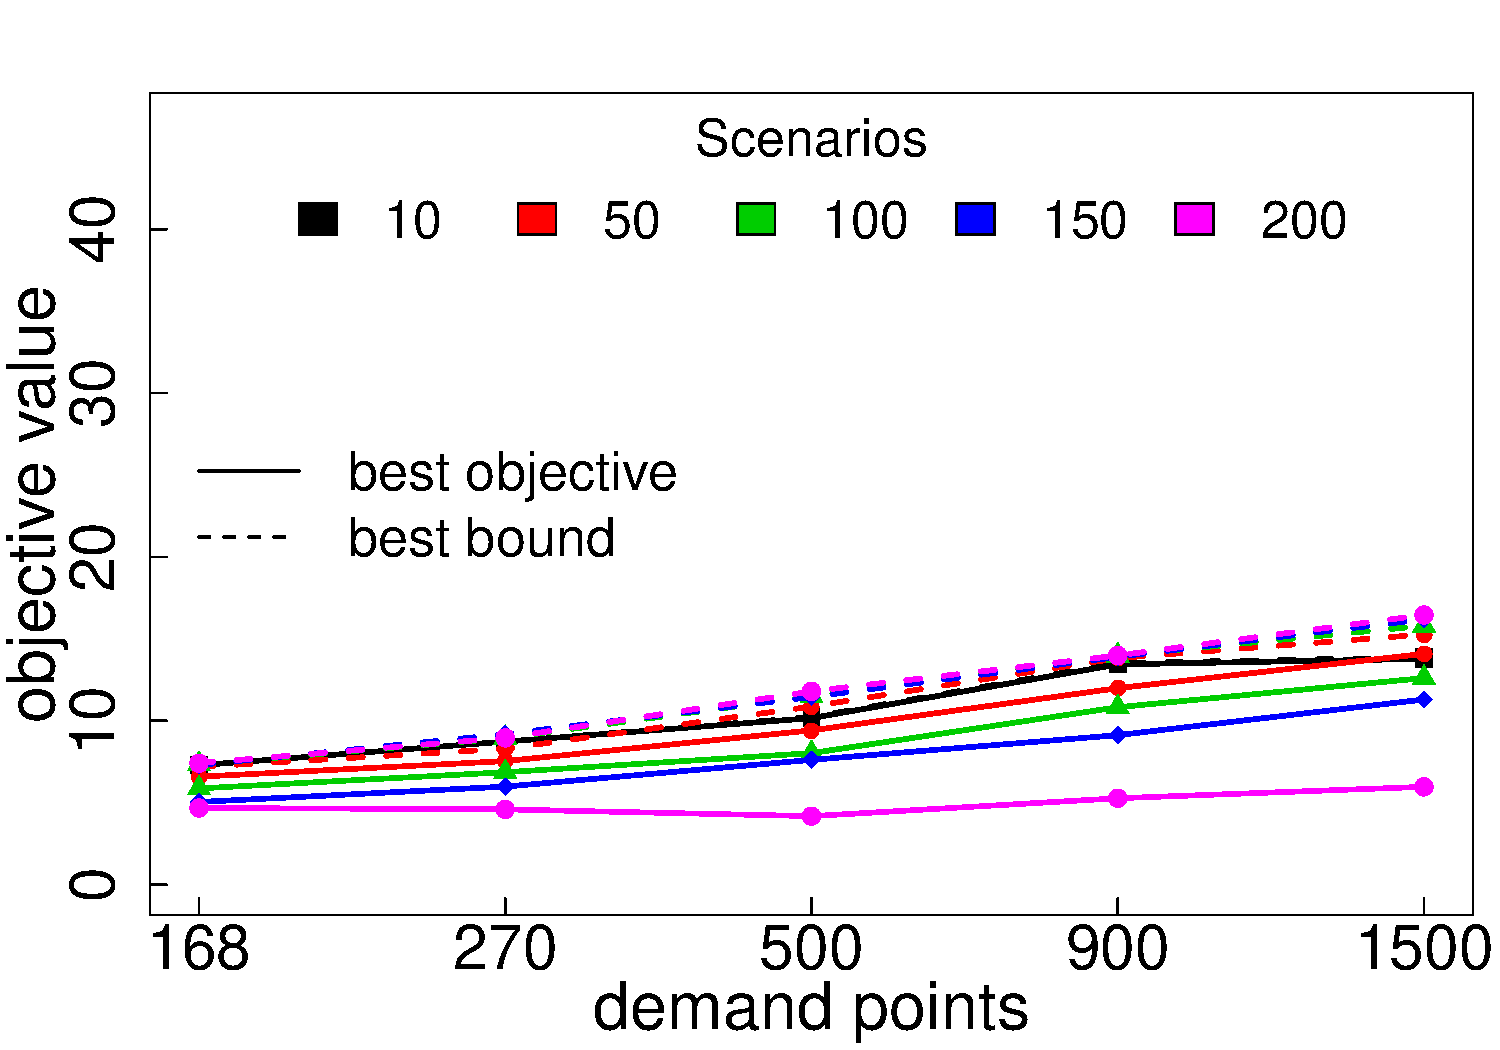
\includegraphics[width=0.42\textwidth]{Imagenes_Tesis/MEC/Obj_MEC_50.pdf}}{$|L|=50$}%
\hspace{0.4cm}%
\vspace{0.4cm}
\stackunder[4pt]{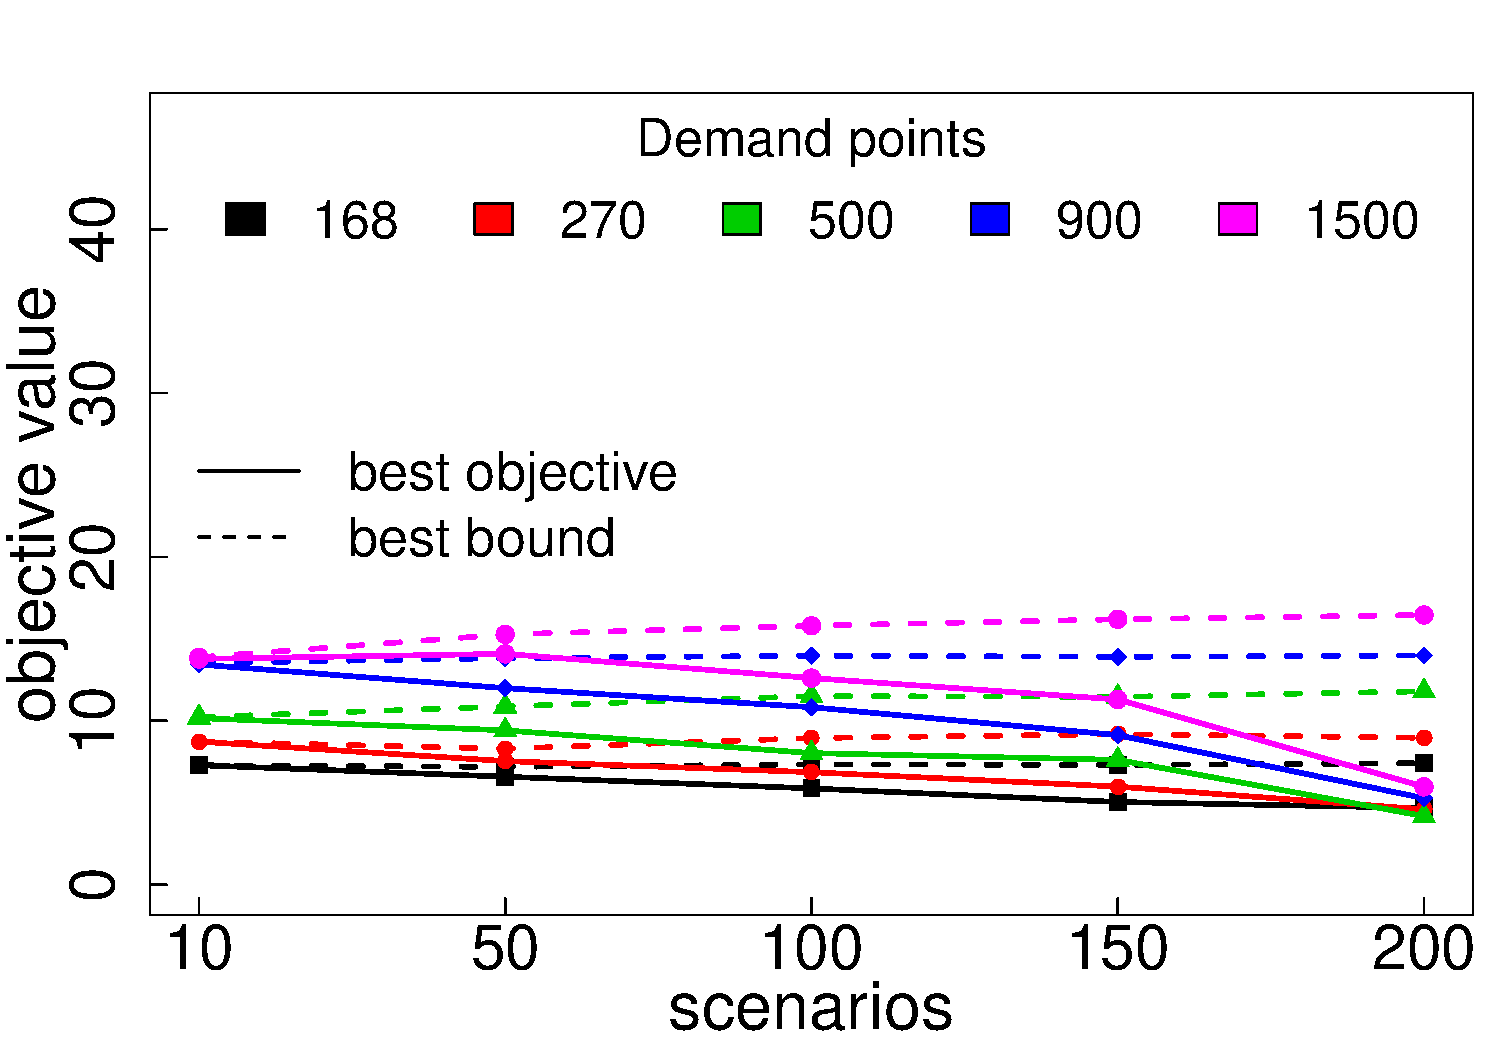
\includegraphics[width=0.42\textwidth]{Imagenes_Tesis/MEC/Obj_MEC_50_1.pdf}}{$|L|=50$}
\stackunder[4pt]{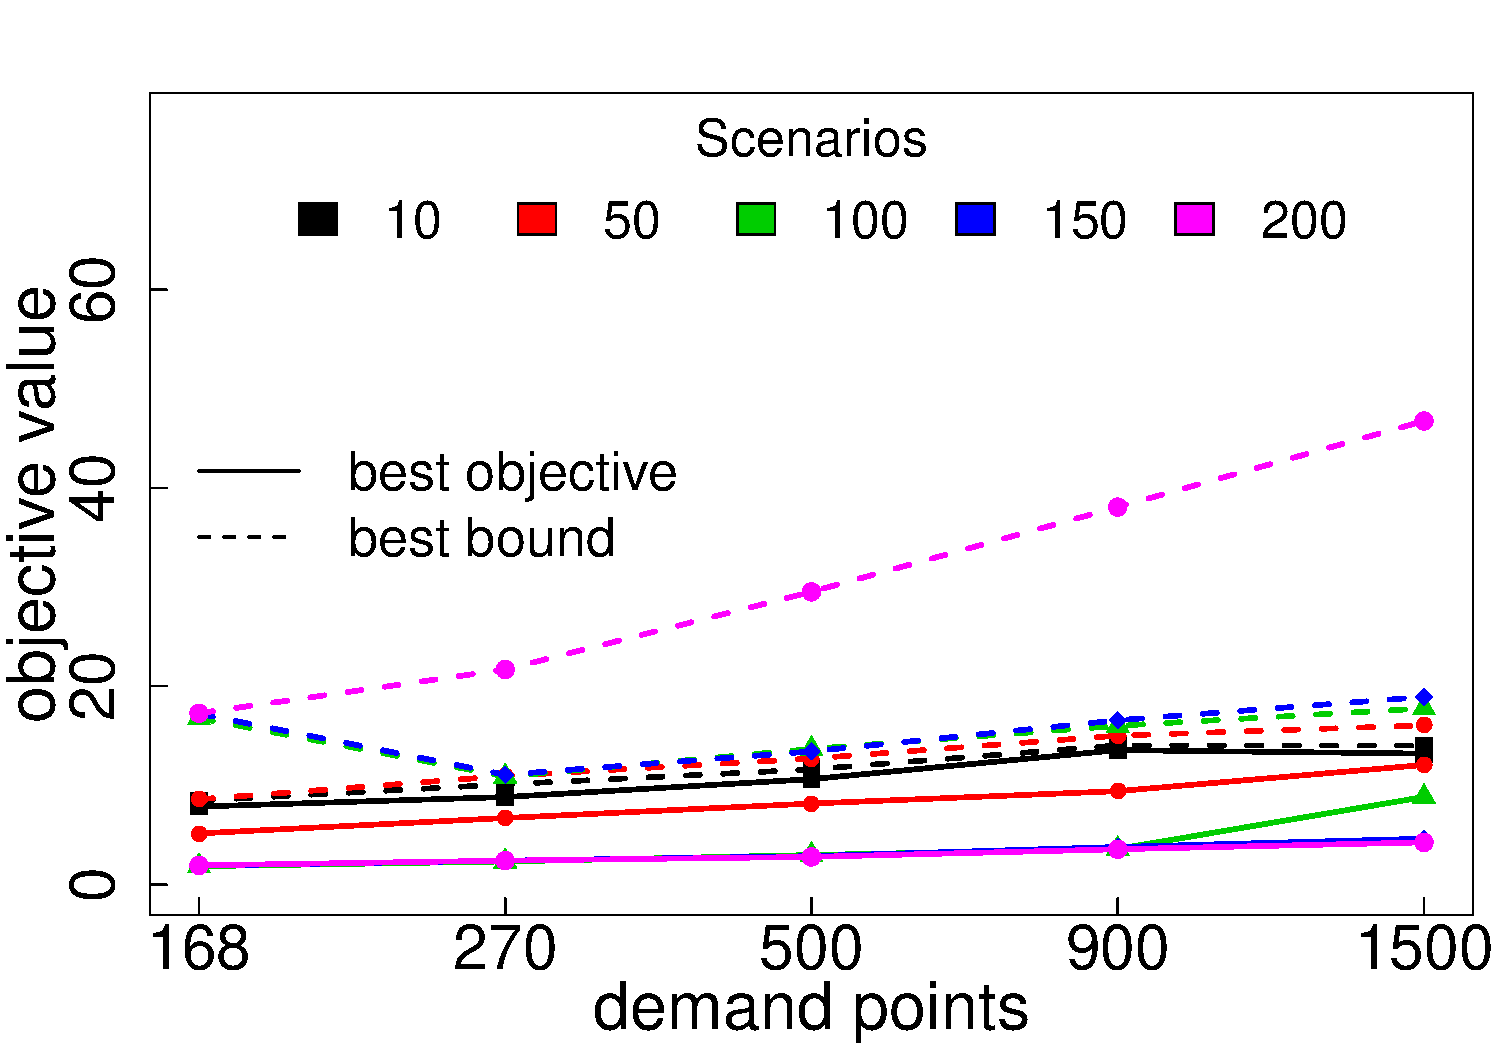
\includegraphics[width=0.42\textwidth]{Imagenes_Tesis/MEC/Obj_MEC_100.pdf}}{$|L|=100$}%
\hspace{0.4cm}%
\vspace{0.4cm}
\stackunder[4pt]{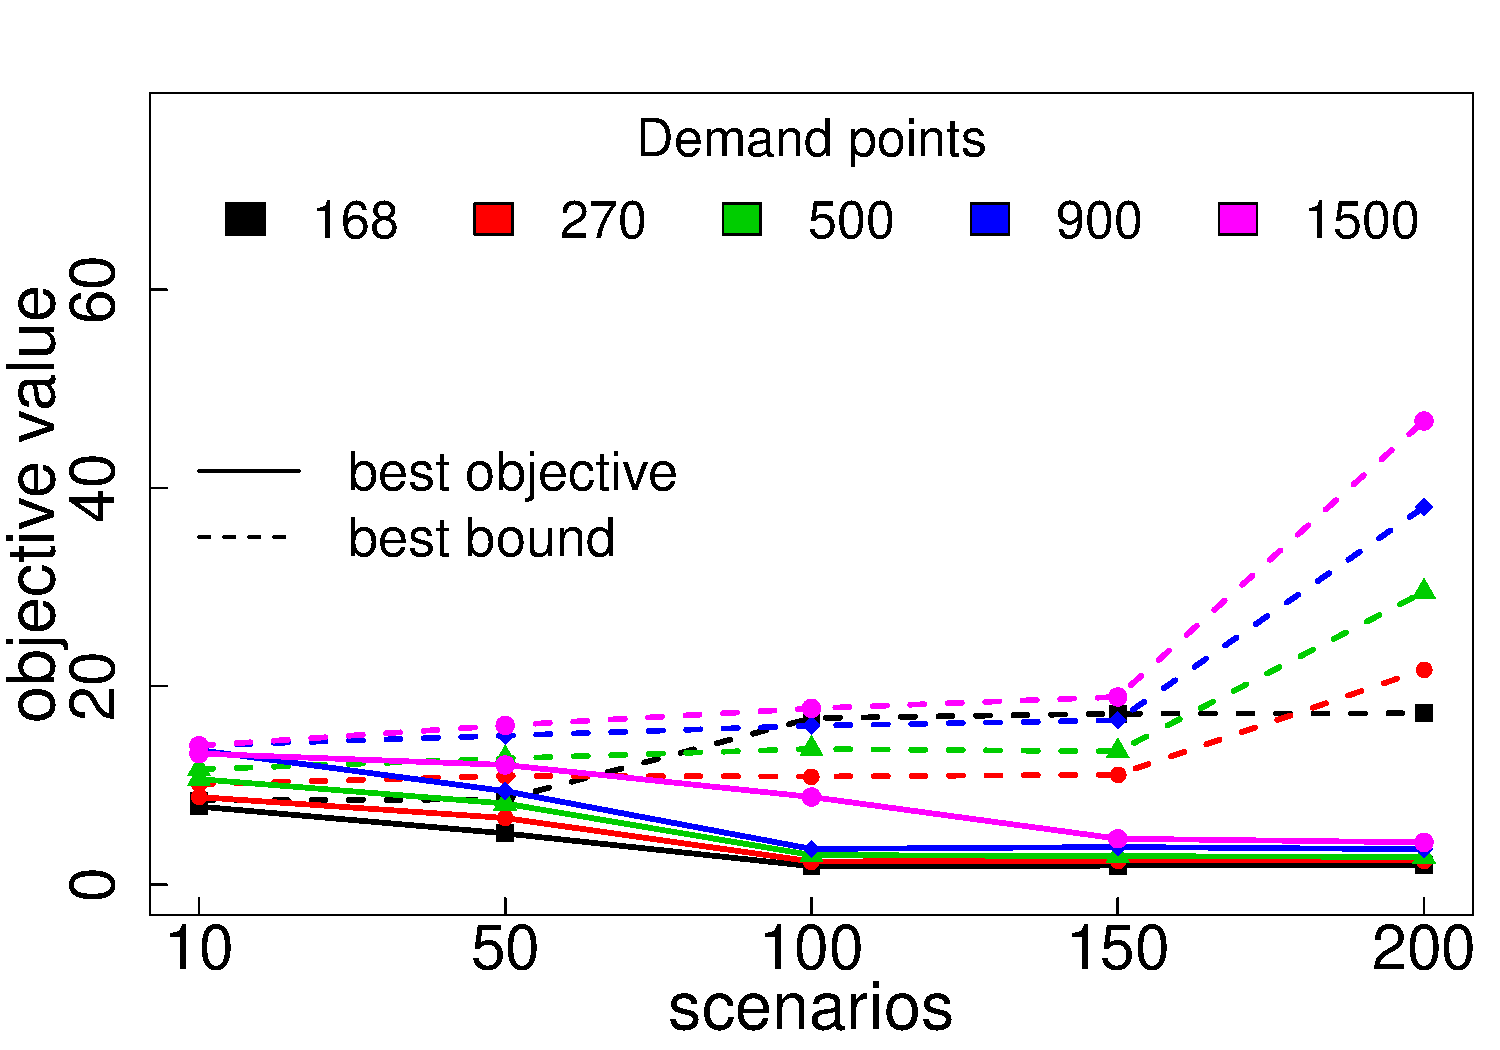
\includegraphics[width=0.42\textwidth]{Imagenes_Tesis/MEC/Obj_MEC_100_1.pdf}}{$|L|=100$}
\caption{Objective values for the MEC problem.}
\label{Obj_MEC}
\end{figure}

As can be seen from the plots, the difference between the best objective and the best bound (and thus, the relative optimality gaps\footnote{(best objective -  best bound)/best objective.}) are negligible for small instances with 16 potential locations sites. Still, the gaps become larger for the instances with 50 and 100 potential sites. The number of demand points where emergencies may occur and the scenarios considered make the instances harder to solve optimally within the time limit. Thus, the deterministic equivalent integer program of MEC can only handle small instances with a few scenarios, demand points (emergency points), and potential ambulance sites. Note that the larger the number of scenarios in the plots on the left-hand side, the better the objective function. This implies that a better sampling of the emergency demand points benefits the quality of the solution related to the ambulance response time. The plots on the right side show that the larger the size of the demand point set, the harder it is to solve the instance. 

   
%\begin{figure}[htb]
%    \centering
%    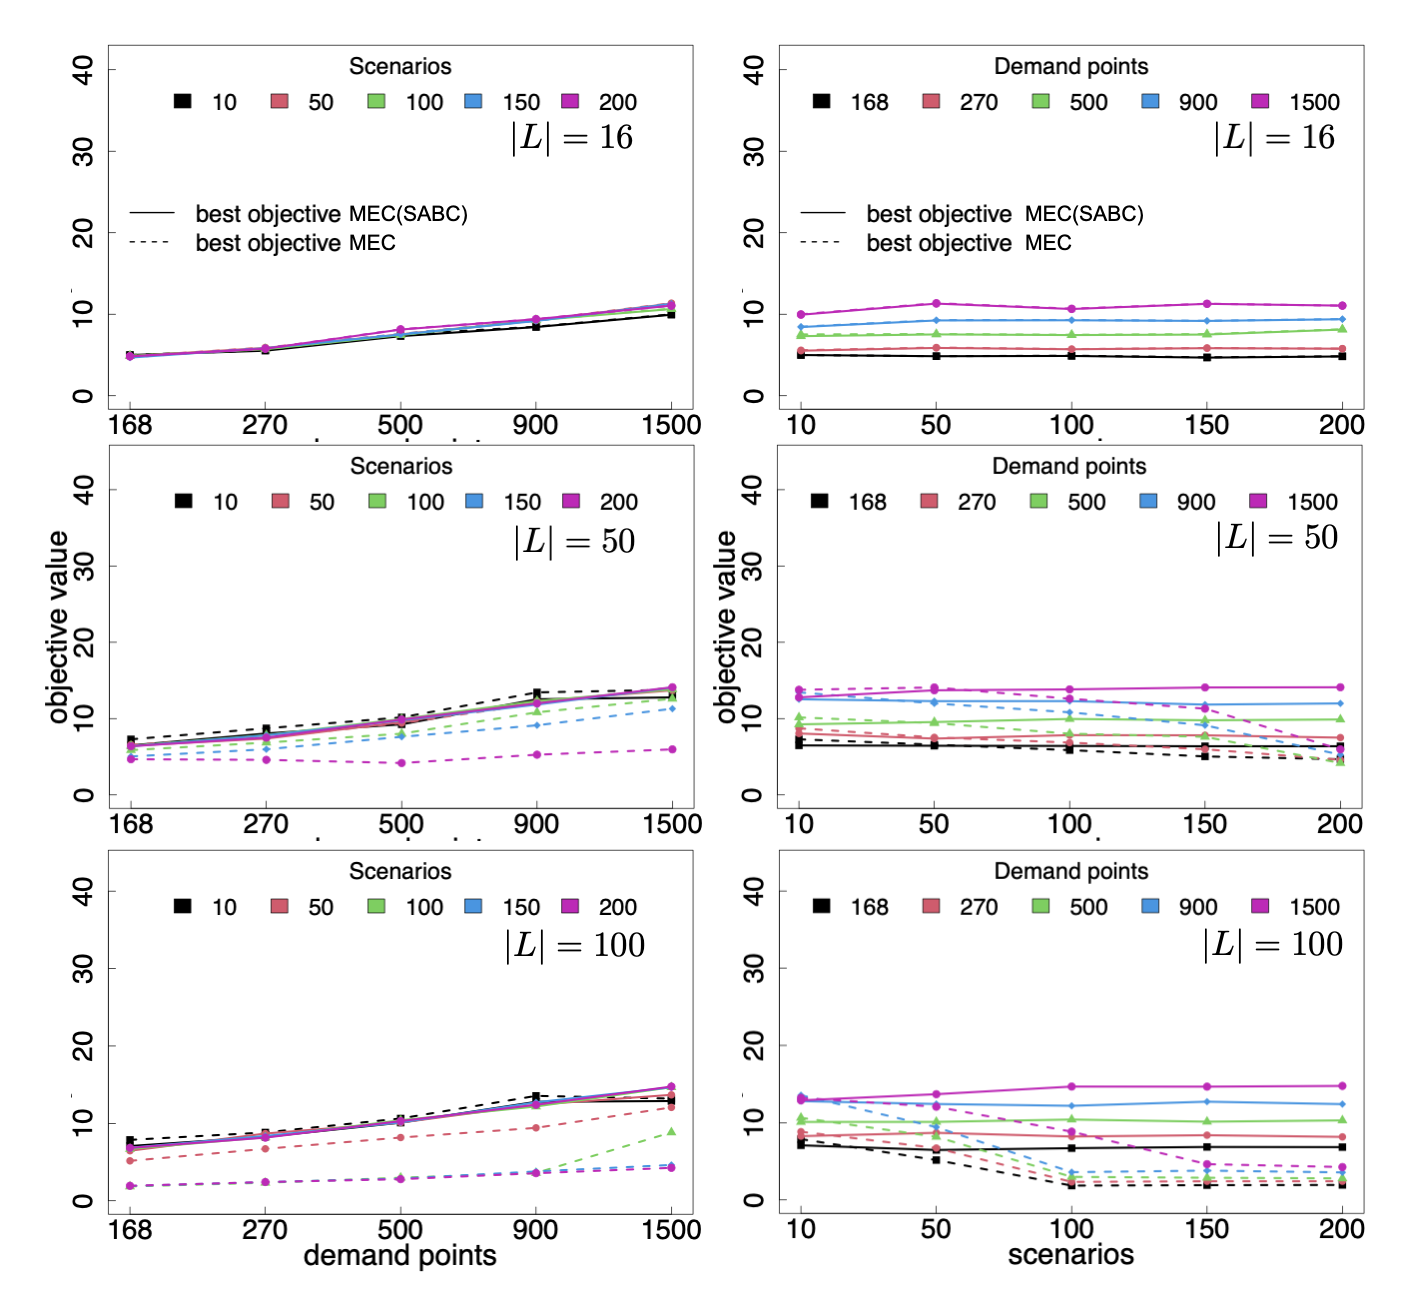
\includegraphics[width=.8\linewidth]{M2M1objectiveValue.png}
%    \caption{Comparison of the best objective values of MEC and MEC(SABC) concerning the demand points on the left side and the scenarios on the right side for different sizes of potential sites $|L|=\{16,50,100\}$.}
%    \label{fig:M2M1objV}
%\end{figure}

For the MEC(SABC) methodology, we have the solution represented in Figure \ref{Obj_M2M1}, which have a similar structure to the previous one. For this methodology, the number of scenarios not affects the results for the objective value due to the MEC(SABC) only considers the ambulances serving the accidents. To this methodology, the optimal is found in a easier and faster way than the MEC, but it is different to the optimal at the MEC so we need to compare the objective values of both of them. 

\begin{figure}[H]
\centering
\footnotesize
\stackunder[4pt]{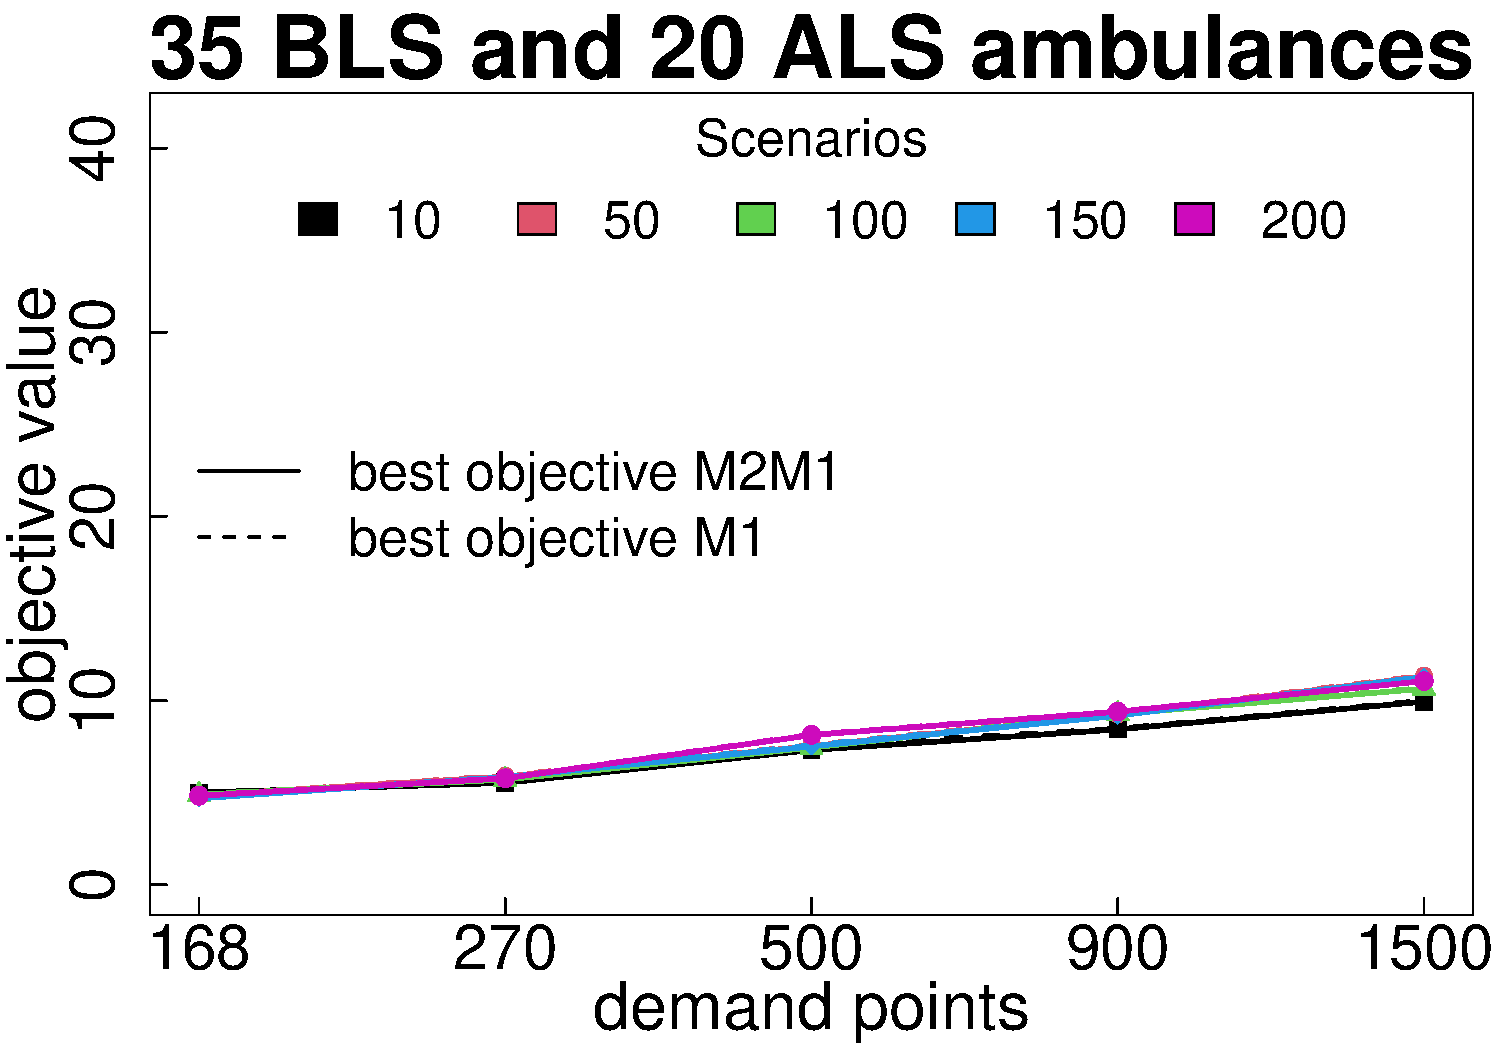
\includegraphics[width=0.42\textwidth]{Imagenes_Tesis/M2M1/Obj_M2M1_16.pdf}}{$|L|=16$}%
\hspace{0.4cm}%
\vspace{0.4cm}
\stackunder[4pt]{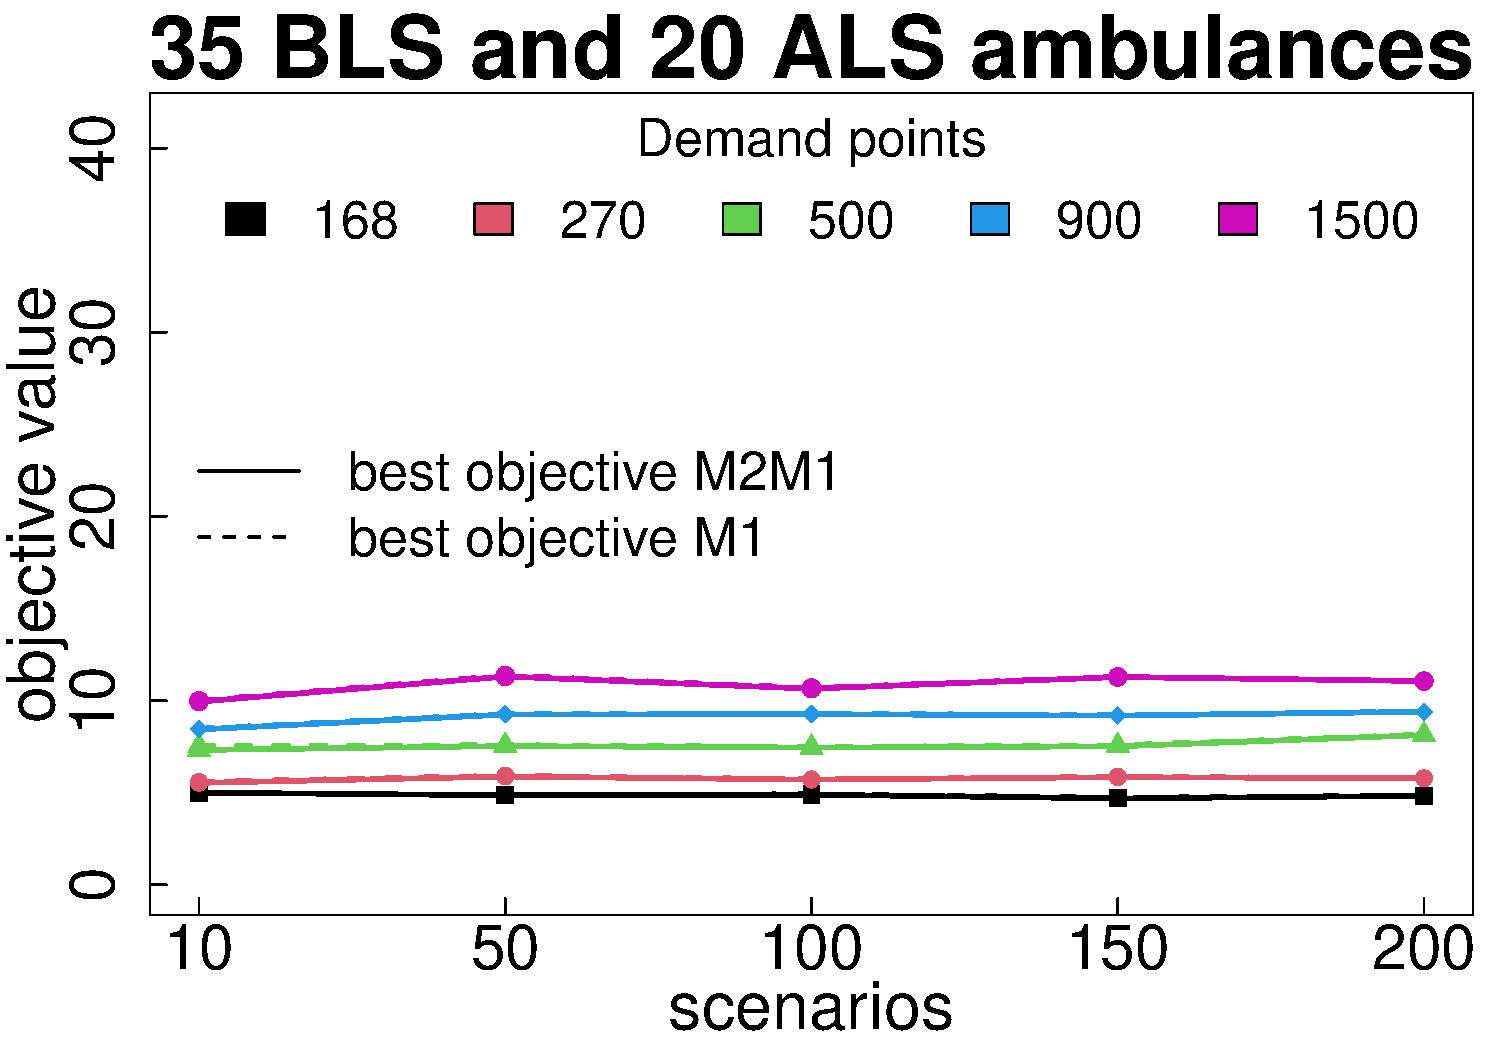
\includegraphics[width=0.42\textwidth]{Imagenes_Tesis/M2M1/Obj_M2M1_16_1.pdf}}{$|L|=16$}
\stackunder[4pt]{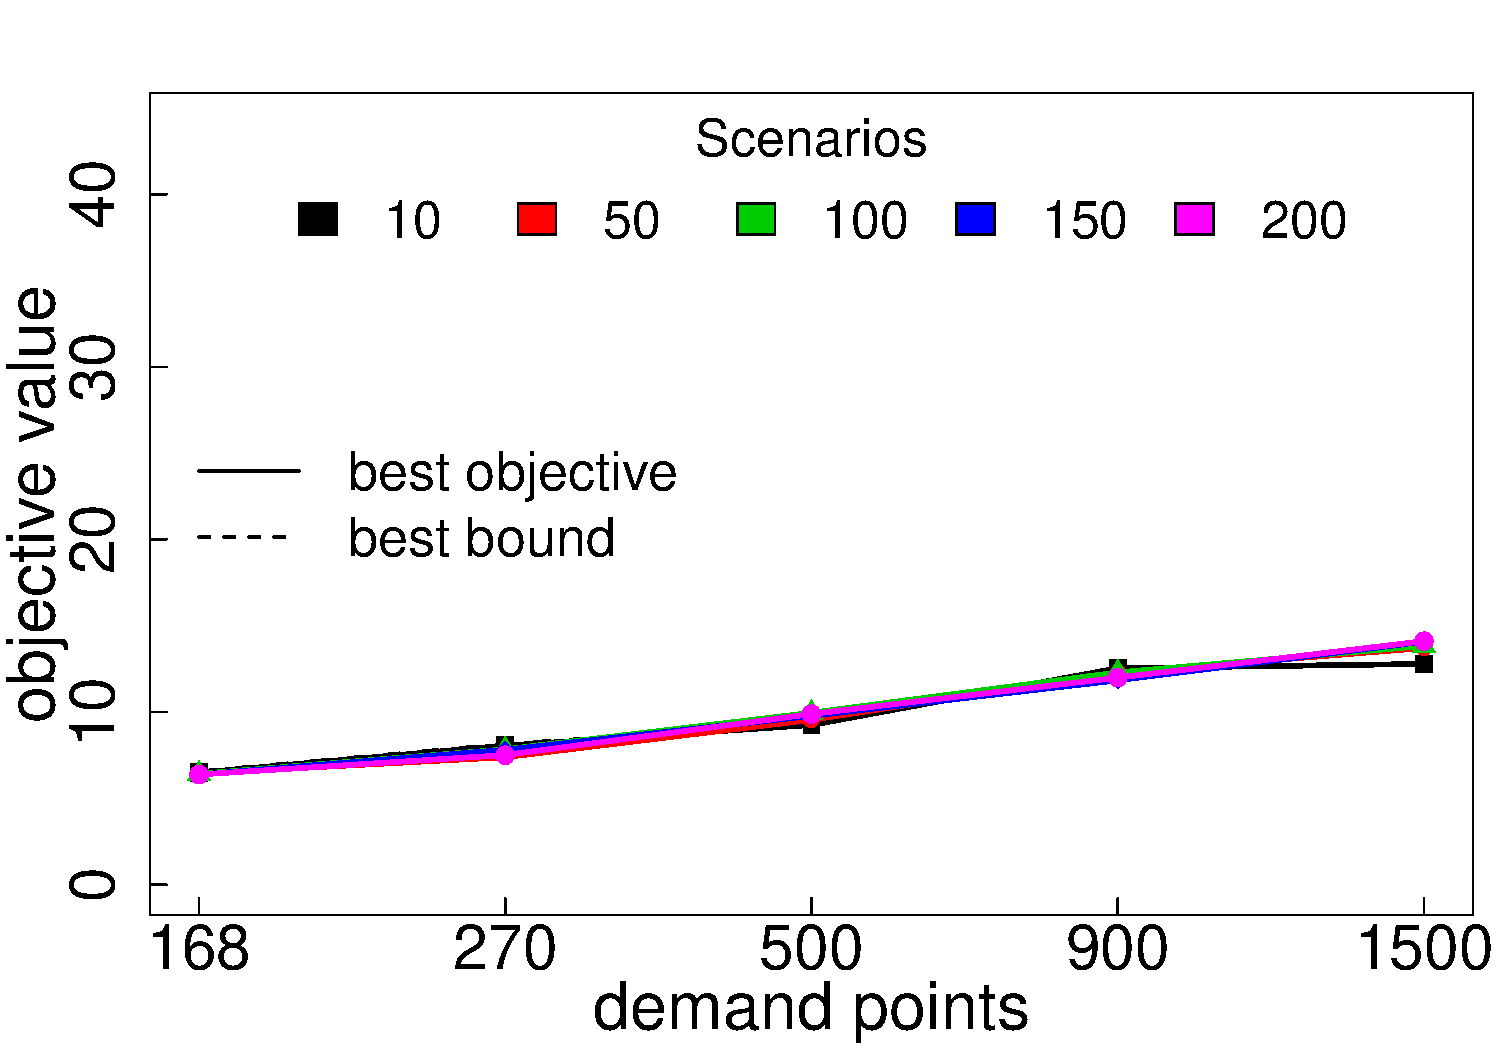
\includegraphics[width=0.42\textwidth]{Imagenes_Tesis/M2M1/Obj_M2M1_50.pdf}}{$|L|=50$}%
\hspace{0.4cm}%
\vspace{0.4cm}
\stackunder[4pt]{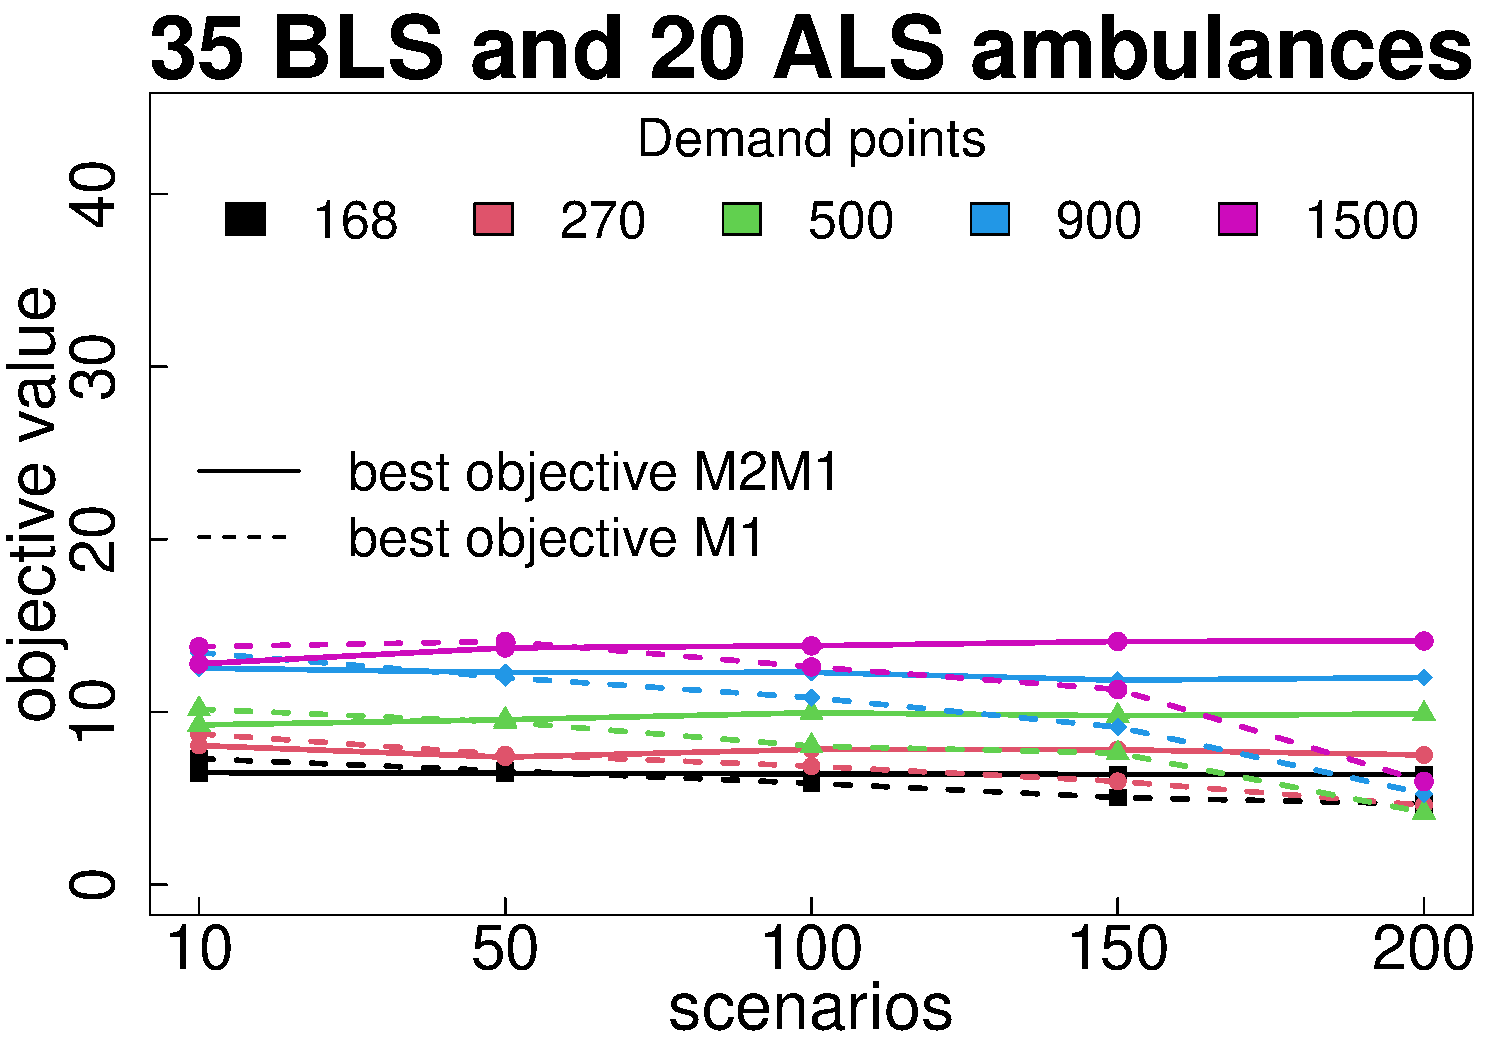
\includegraphics[width=0.42\textwidth]{Imagenes_Tesis/M2M1/Obj_M2M1_50_1.pdf}}{$|L|=50$}
\stackunder[4pt]{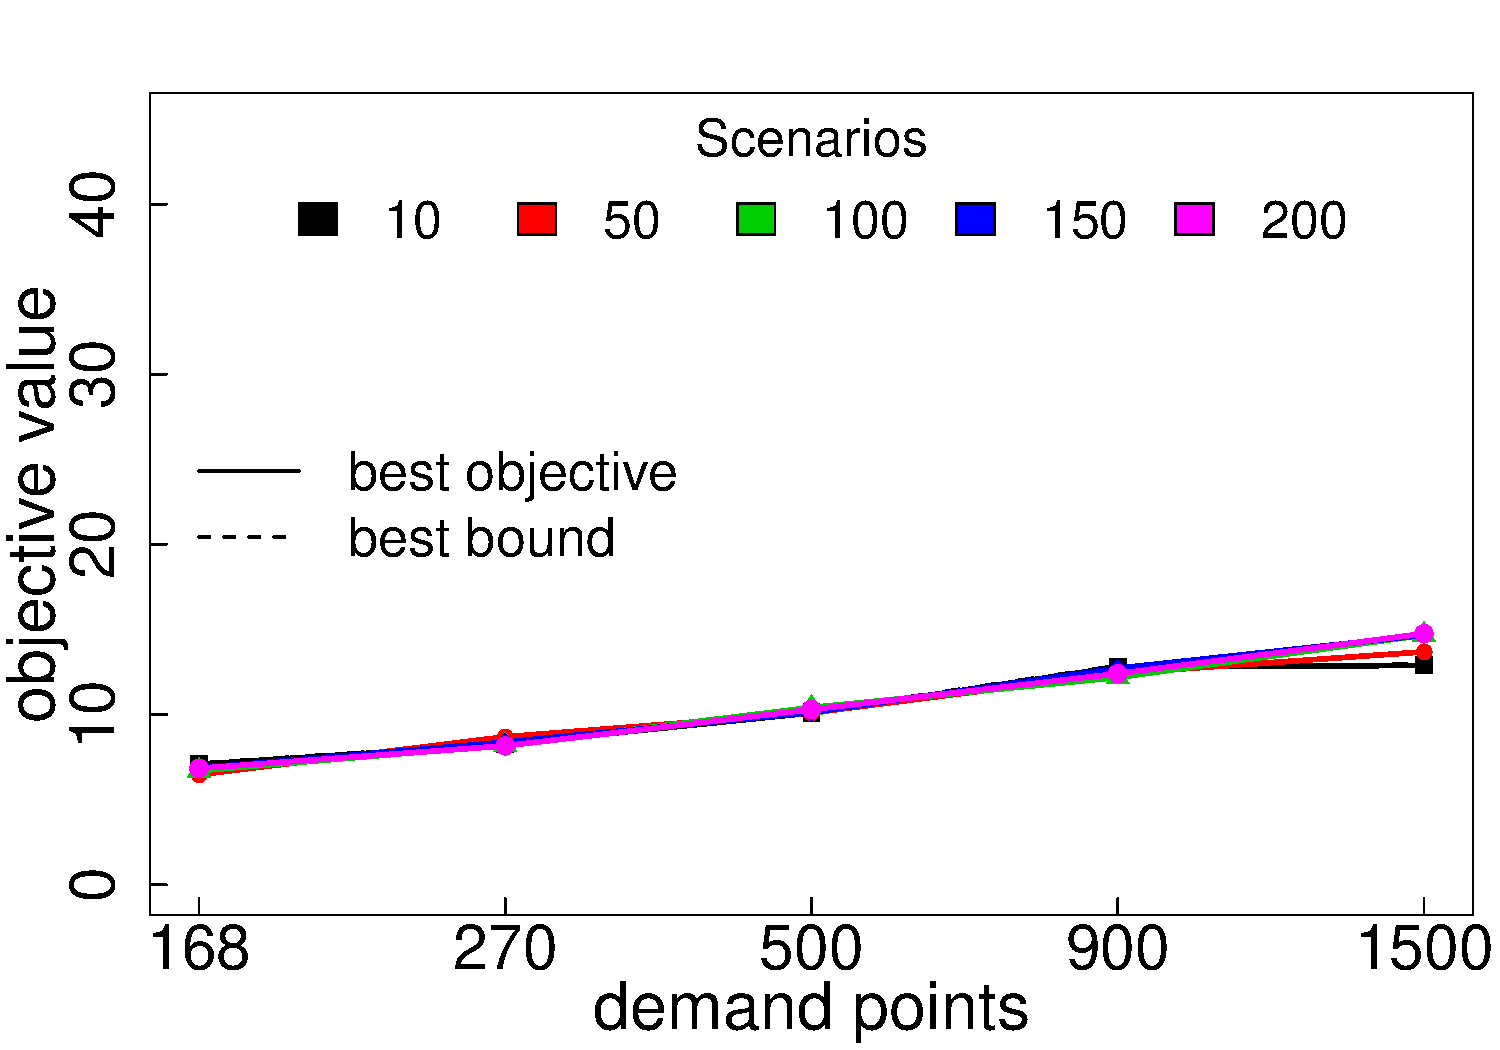
\includegraphics[width=0.42\textwidth]{Imagenes_Tesis/M2M1/Obj_M2M1_100.pdf}}{$|L|=100$}%
\hspace{0.4cm}%
\vspace{0.4cm}
\stackunder[4pt]{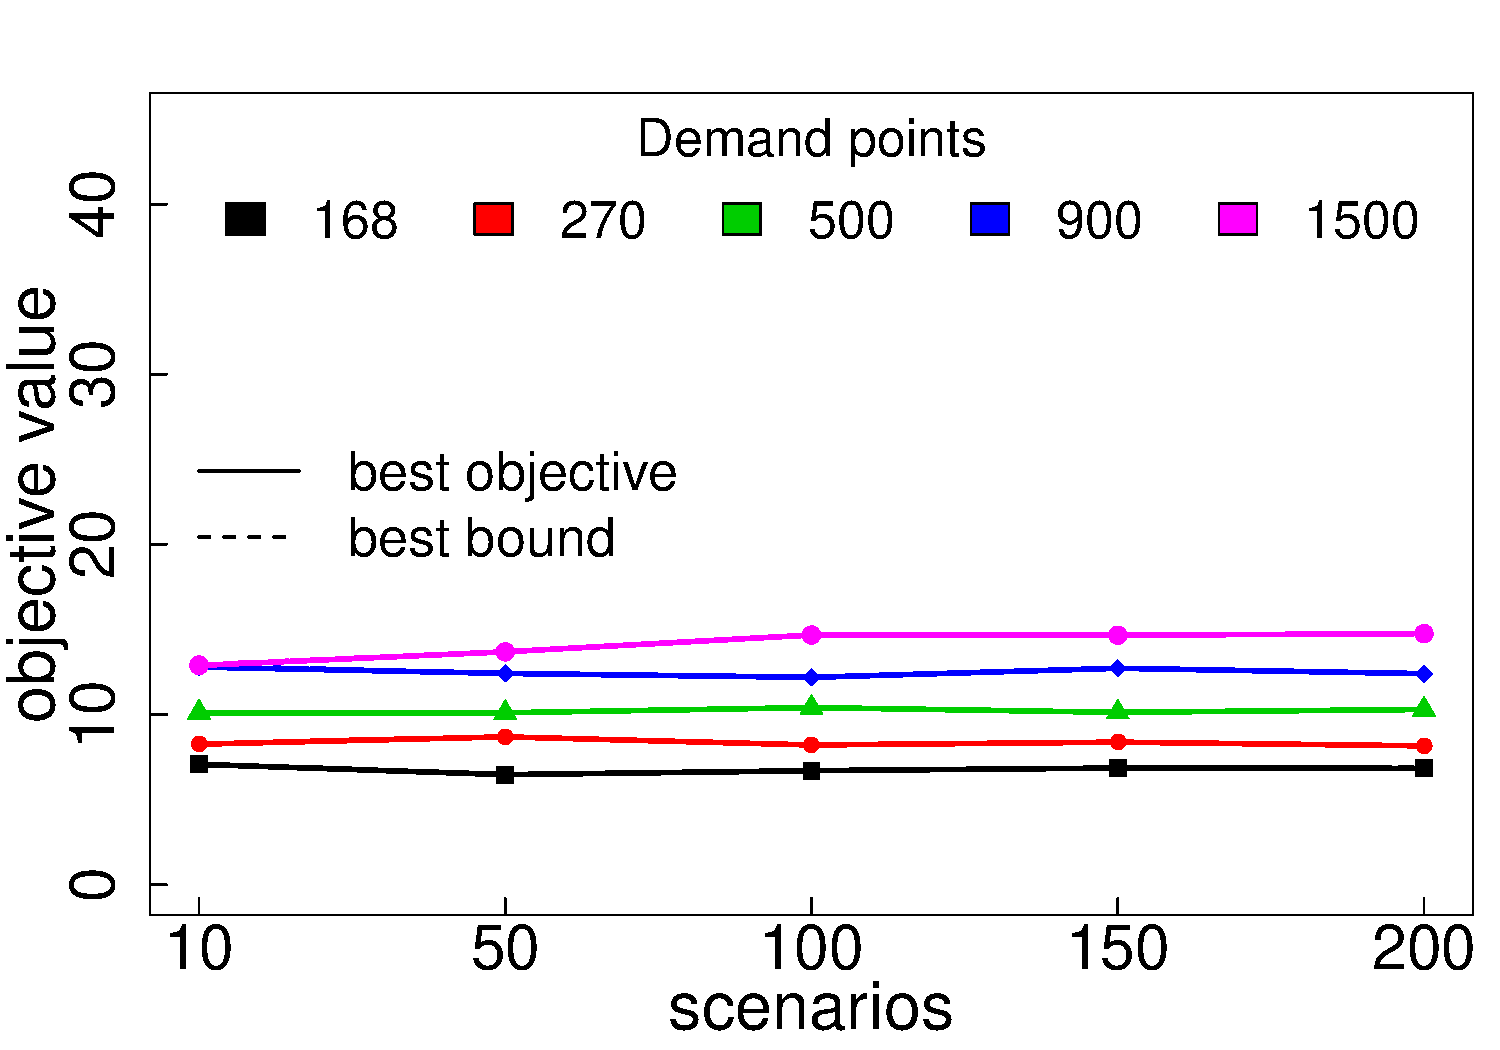
\includegraphics[width=0.42\textwidth]{Imagenes_Tesis/M2M1/Obj_M2M1_100_1.pdf}}{$|L|=100$}
\caption{Objective values for the MEC(SABC) methodology.}
\label{Obj_M2M1}
\end{figure}

Now, we compare the solution values of the equivalent integer program of MEC with the ones obtained by MEC(SABC) in Figure \ref{Obj_M2M1-M1}. As can be seen, while the number of scenarios, demand points, and potential sites slightly affects the performance of MEC(SABC), it obtains better objective function values than those obtained by the MEC model for the larger instances that reported positive gaps. Indeed, the optimality gaps of the MEC(SABC) model always equal 0 within the time limit that we established. In addition, the MEC(SABC) model tends to be less dependent on the number of scenarios. Thus, although we cannot guarantee optimality with the MEC(SABC) model, it obtains faster and higher-quality solutions than those obtained by the MEC equivalent model. 


\begin{figure}[H]
\centering
\footnotesize
\stackunder[4pt]{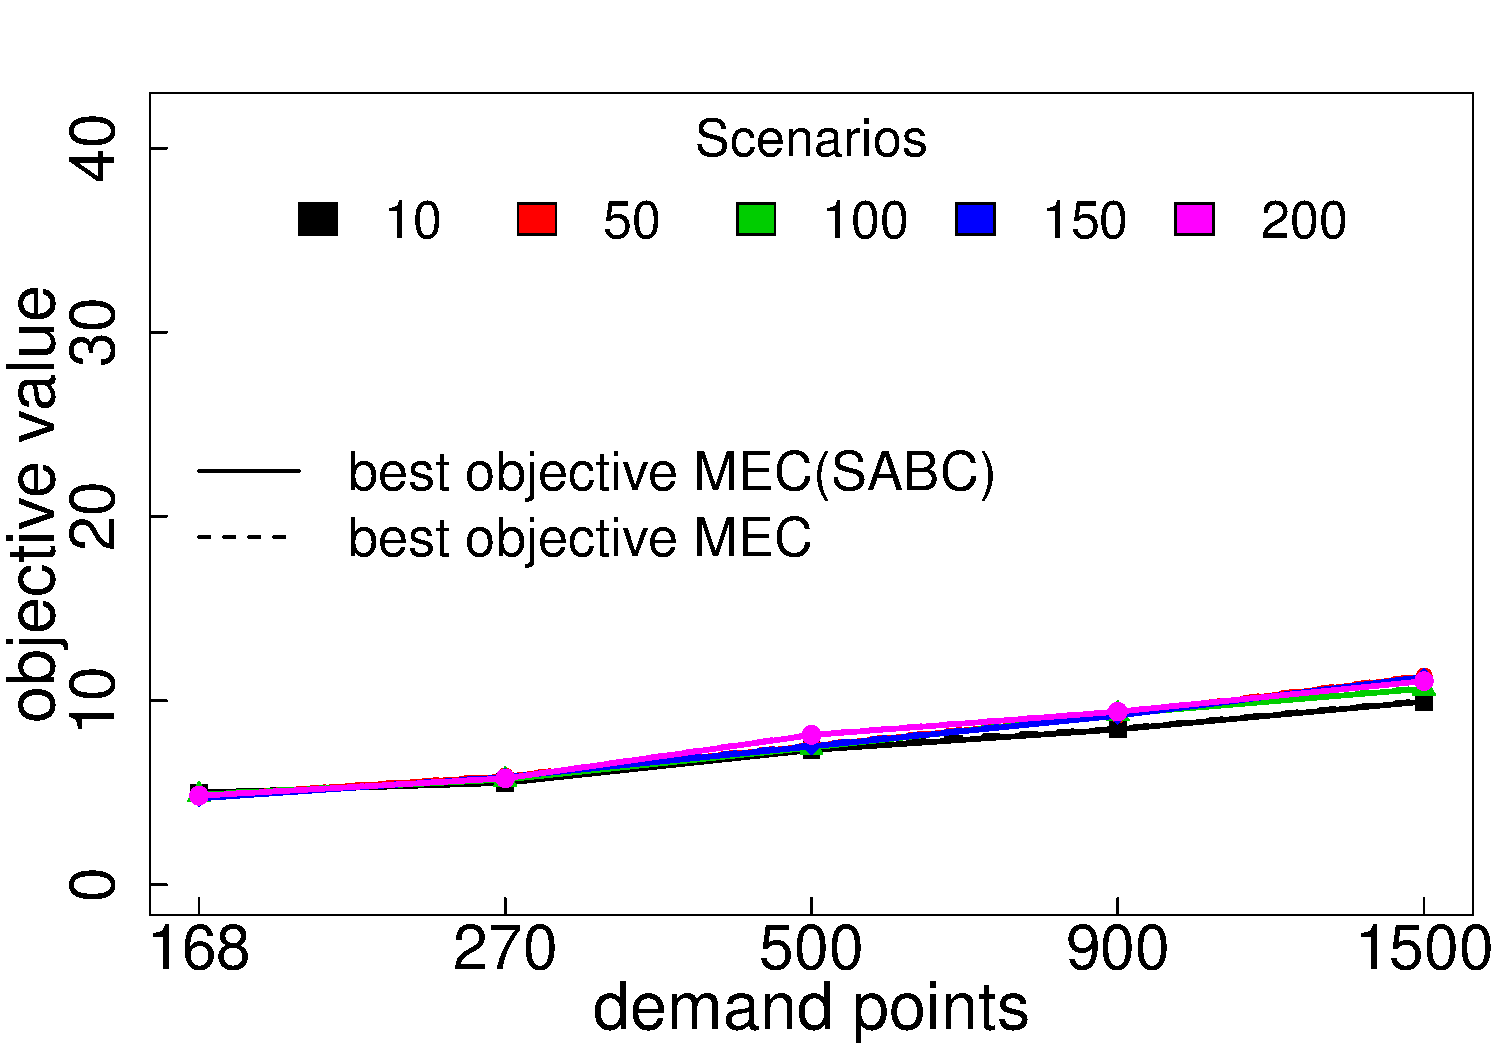
\includegraphics[width=0.42\textwidth]{Imagenes_Tesis/M2M1-M1/Obj_M2M1-M1_16.pdf}}{$|L|=16$}%
\hspace{0.4cm}%
\vspace{0.4cm}
\stackunder[4pt]{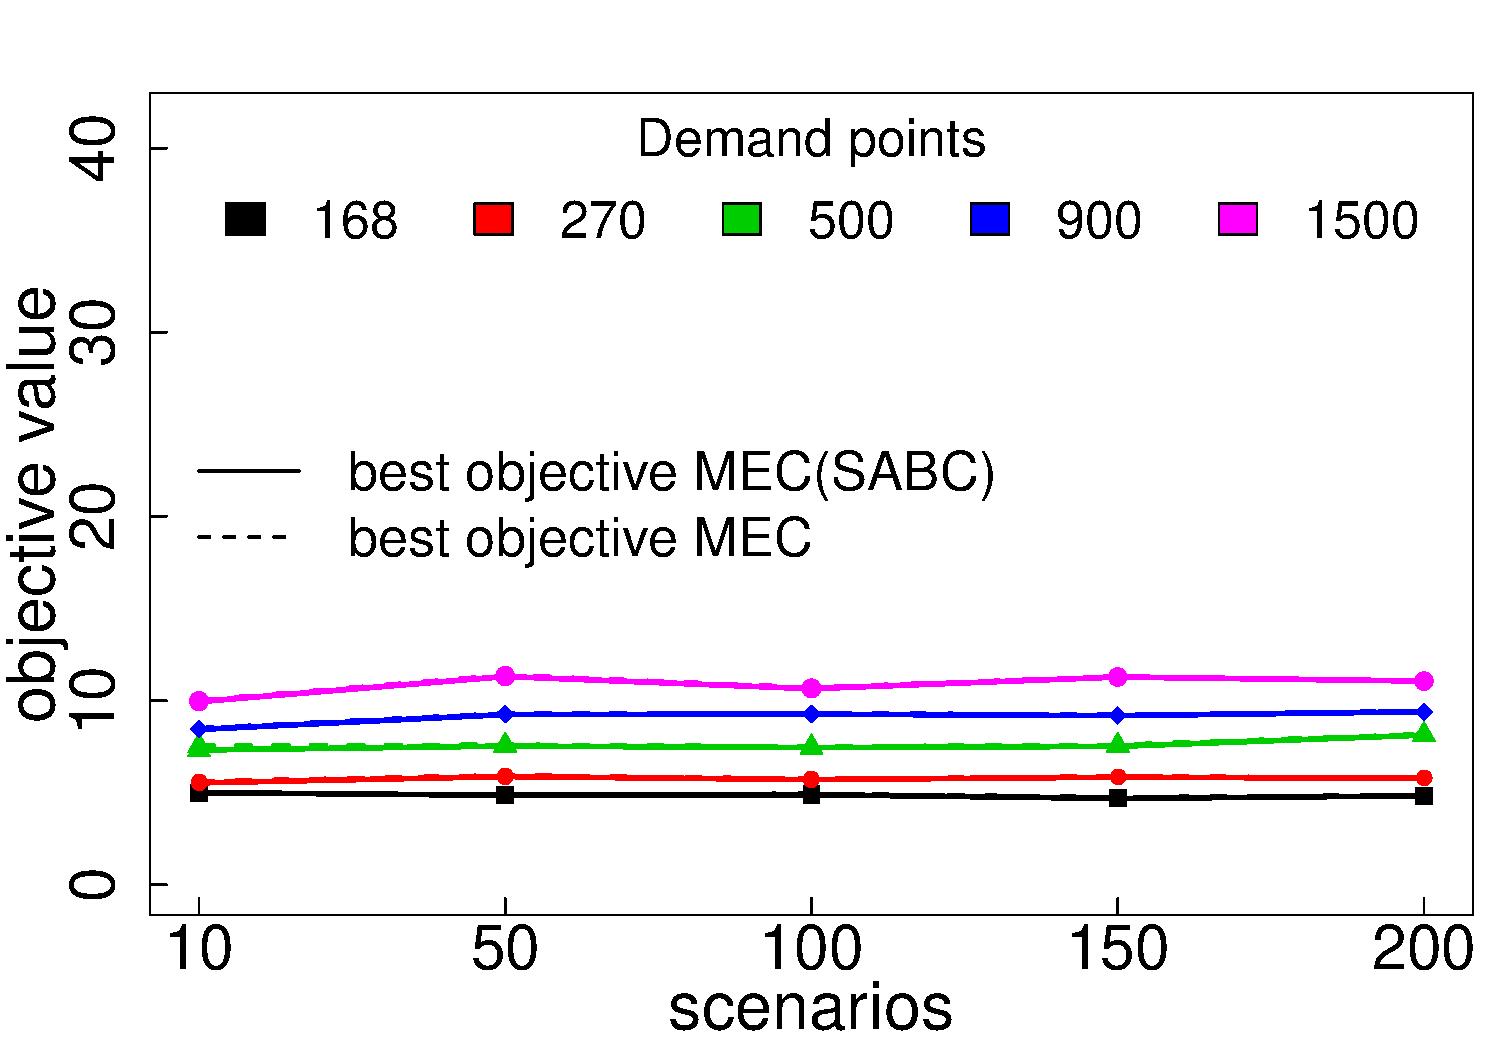
\includegraphics[width=0.42\textwidth]{Imagenes_Tesis/M2M1-M1/Obj_M2M1-M1_16_1.pdf}}{$|L|=16$}
\stackunder[4pt]{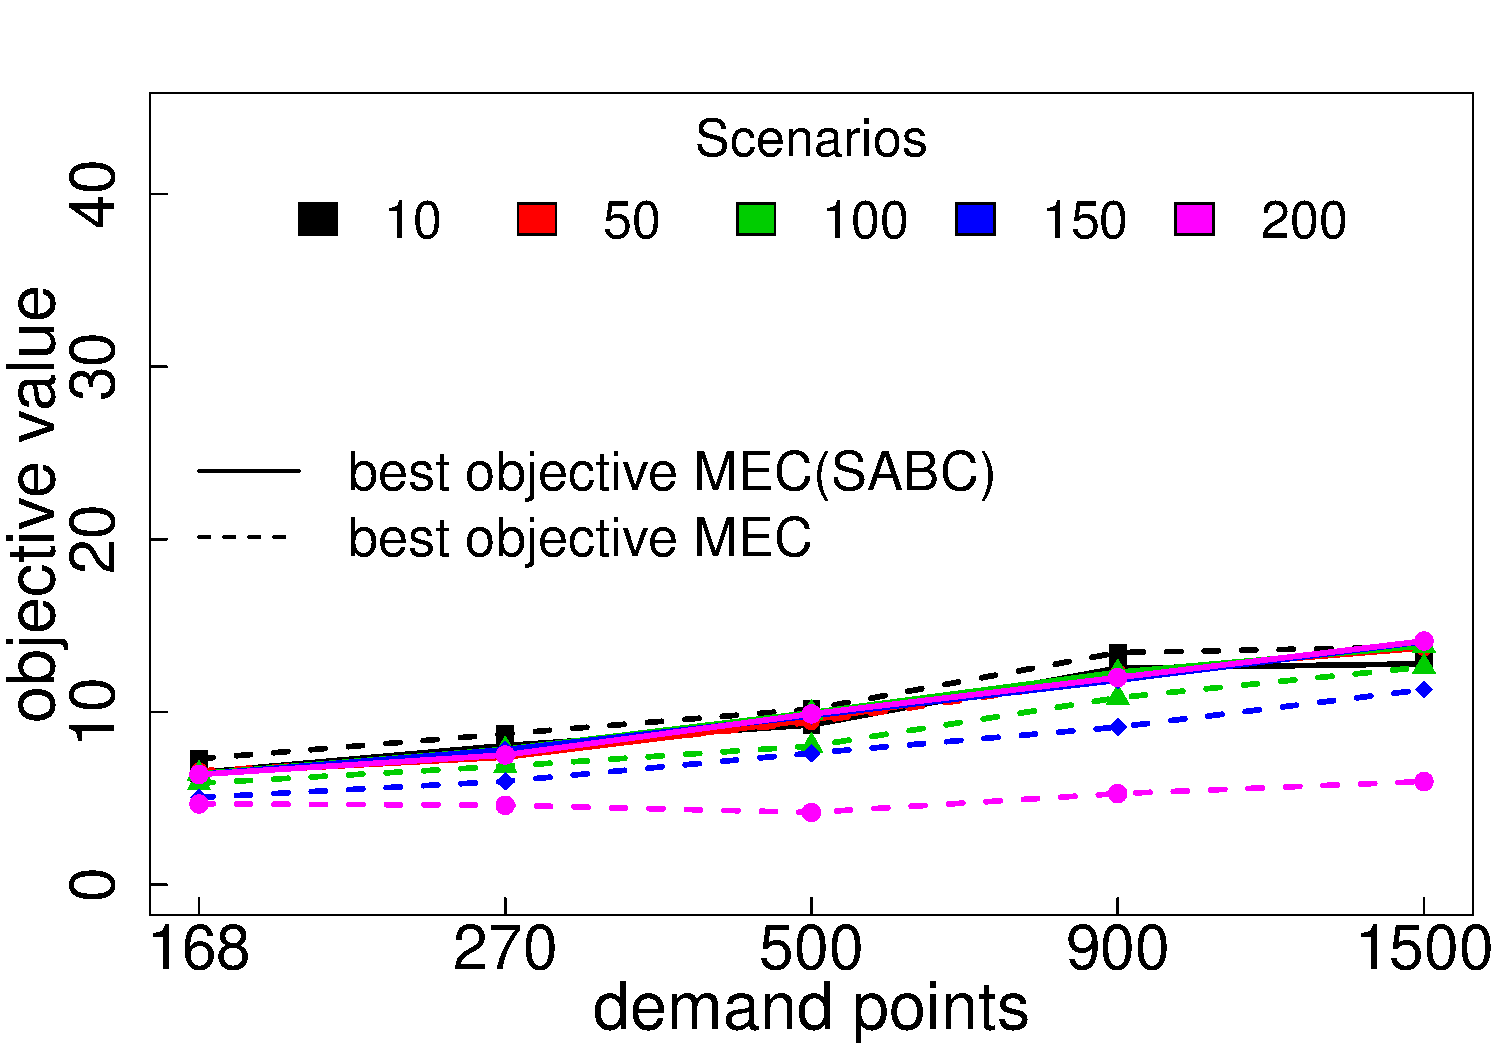
\includegraphics[width=0.42\textwidth]{Imagenes_Tesis/M2M1-M1/Obj_M2M1-M1_50.pdf}}{$|L|=50$}%
\hspace{0.4cm}%
\vspace{0.4cm}
\stackunder[4pt]{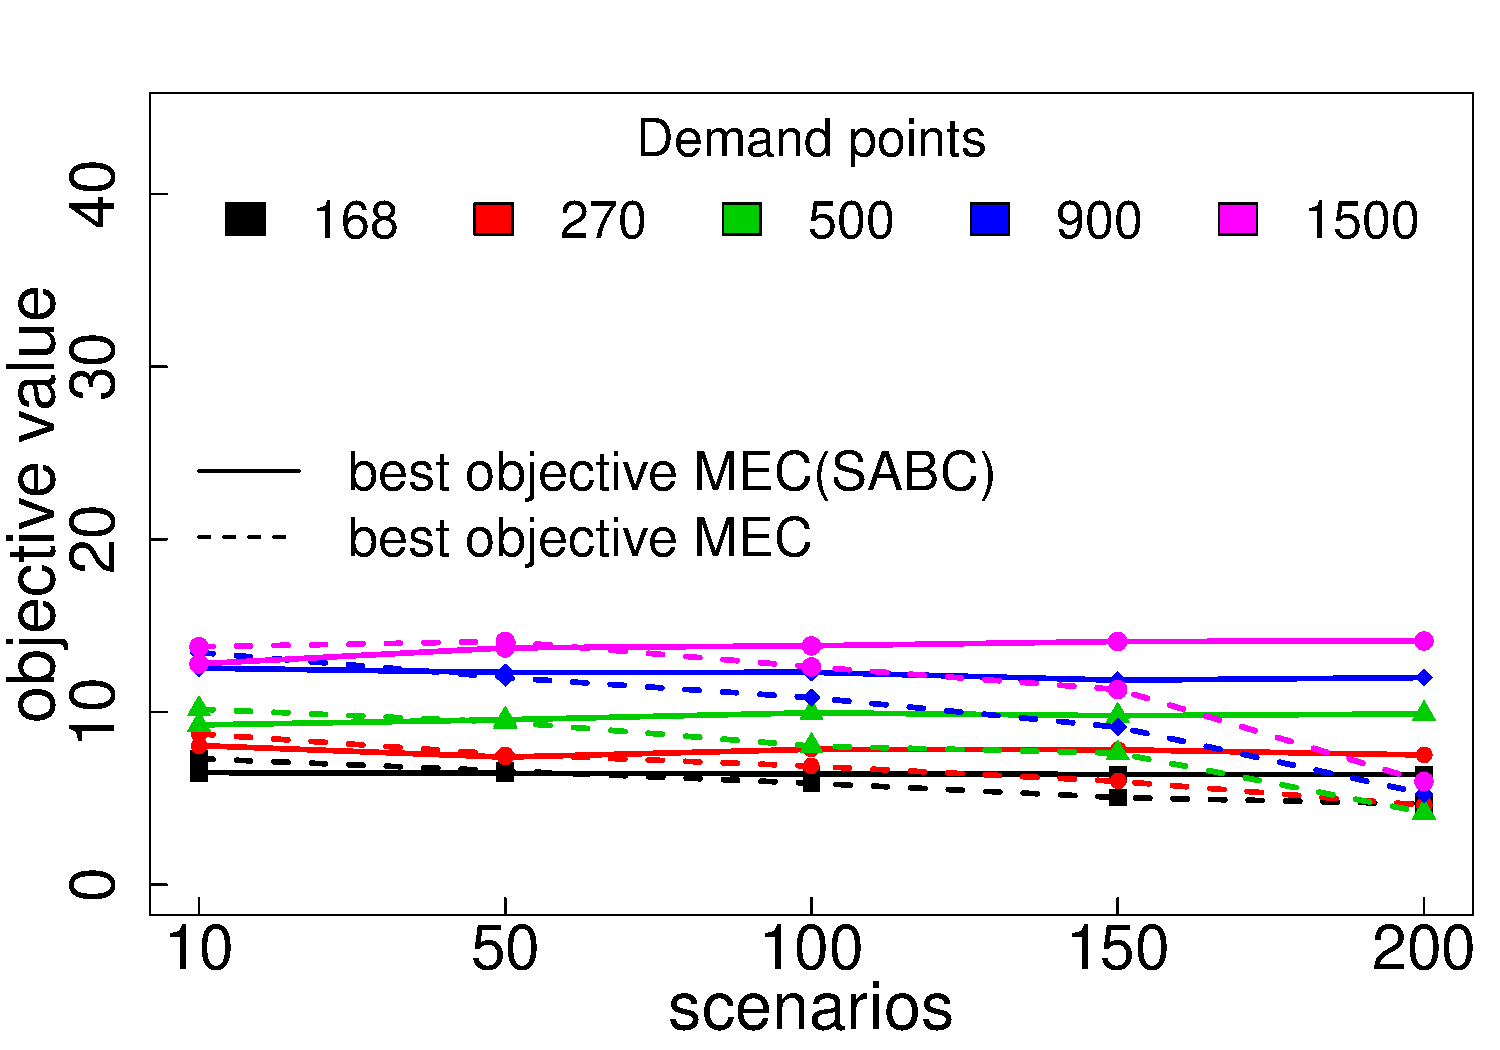
\includegraphics[width=0.42\textwidth]{Imagenes_Tesis/M2M1-M1/Obj_M2M1-M1_50_1.pdf}}{$|L|=50$}
\stackunder[4pt]{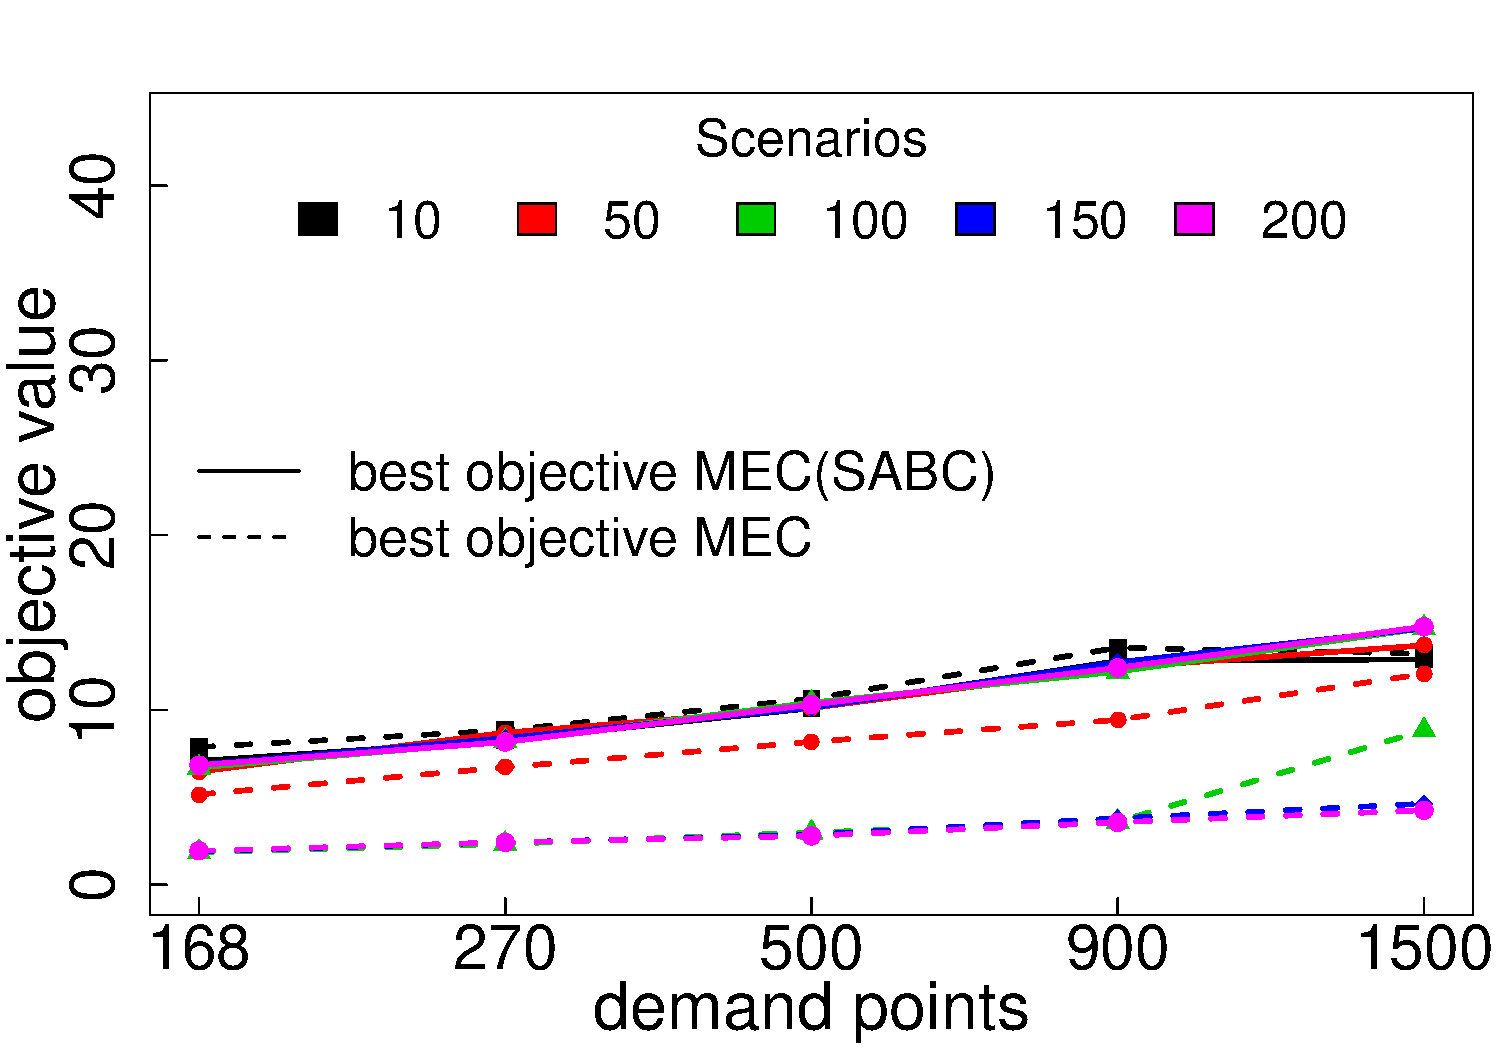
\includegraphics[width=0.42\textwidth]{Imagenes_Tesis/M2M1-M1/Obj_M2M1-M1_100.pdf}}{$|L|=100$}%
\hspace{0.4cm}%
\vspace{0.4cm}
\stackunder[4pt]{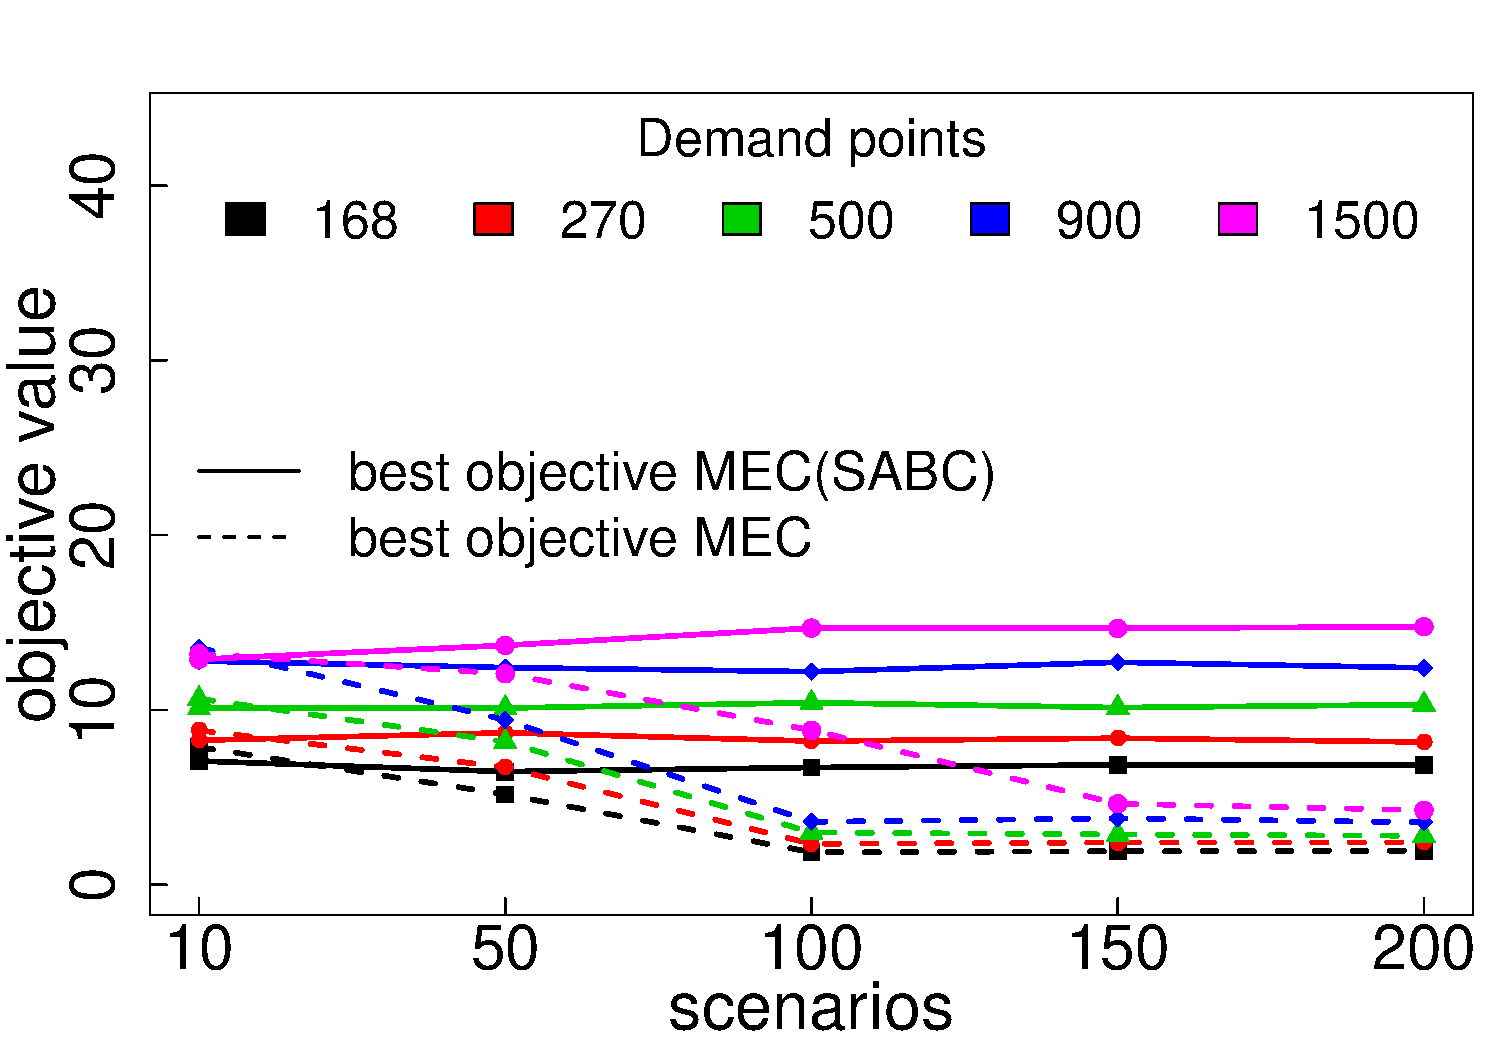
\includegraphics[width=0.42\textwidth]{Imagenes_Tesis/M2M1-M1/Obj_M2M1-M1_100_1.pdf}}{$|L|=100$}
\caption{Objective values of MEC(SABC).}
\label{Obj_M2M1-M1}
\end{figure}

Once we analyze the MEC(SABC) we have in Figure \ref{Obj_Math} the SABC Matheuristic results. The axis on the left-hand and the right-hand sides of the Figure can be described as previous ones. Straight lines indicates the best objective value found throughout the Matheuristic, i.e. the solution for the best neighbor found from the four neighborhoods explored. As we can see, even for the larger scenarios, we can obtain a solution close to the best bound, which is represented by none straight lines. This means that fixing locations facilitates the exploration in the second stage of the MEC and solutions for Matheuristic can be found efficiently. Although, we need to compare this solutions with the solutions from the MEC and MEC(SABC) to evaluate this mat heuristic.

\begin{figure}[H]
\centering
\footnotesize
\stackunder[4pt]{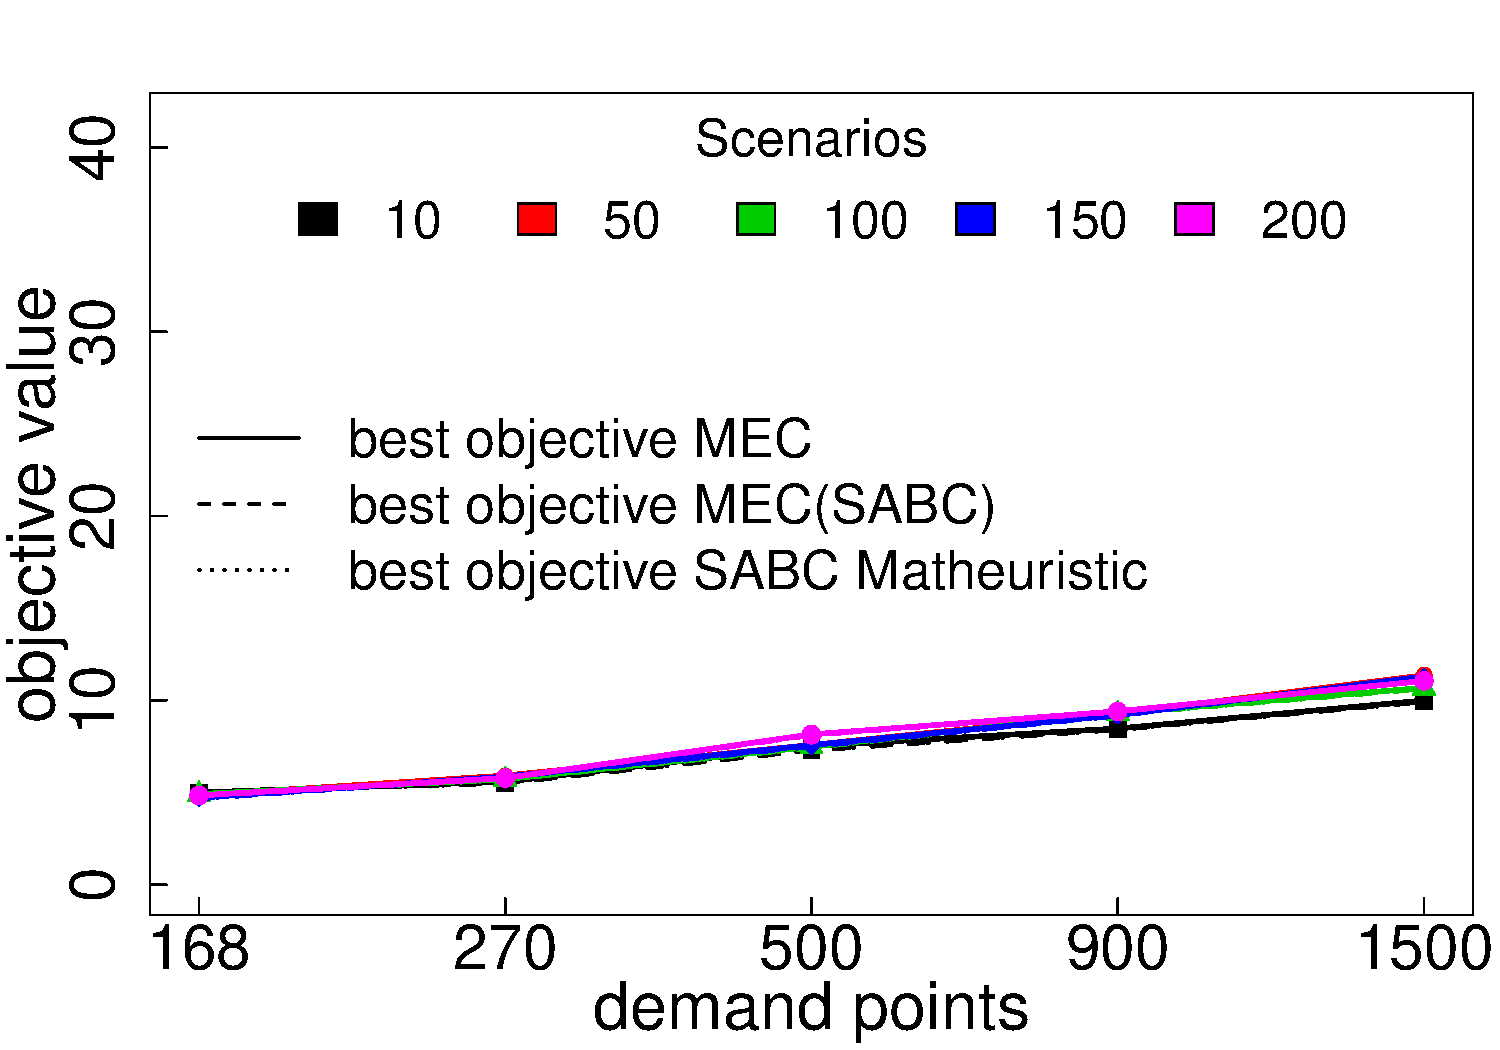
\includegraphics[width=0.42\textwidth]{Imagenes_Tesis/Math/Obj_Math_16.pdf}}{$|L|=16$}%
\hspace{0.4cm}%
\vspace{0.4cm}
\stackunder[4pt]{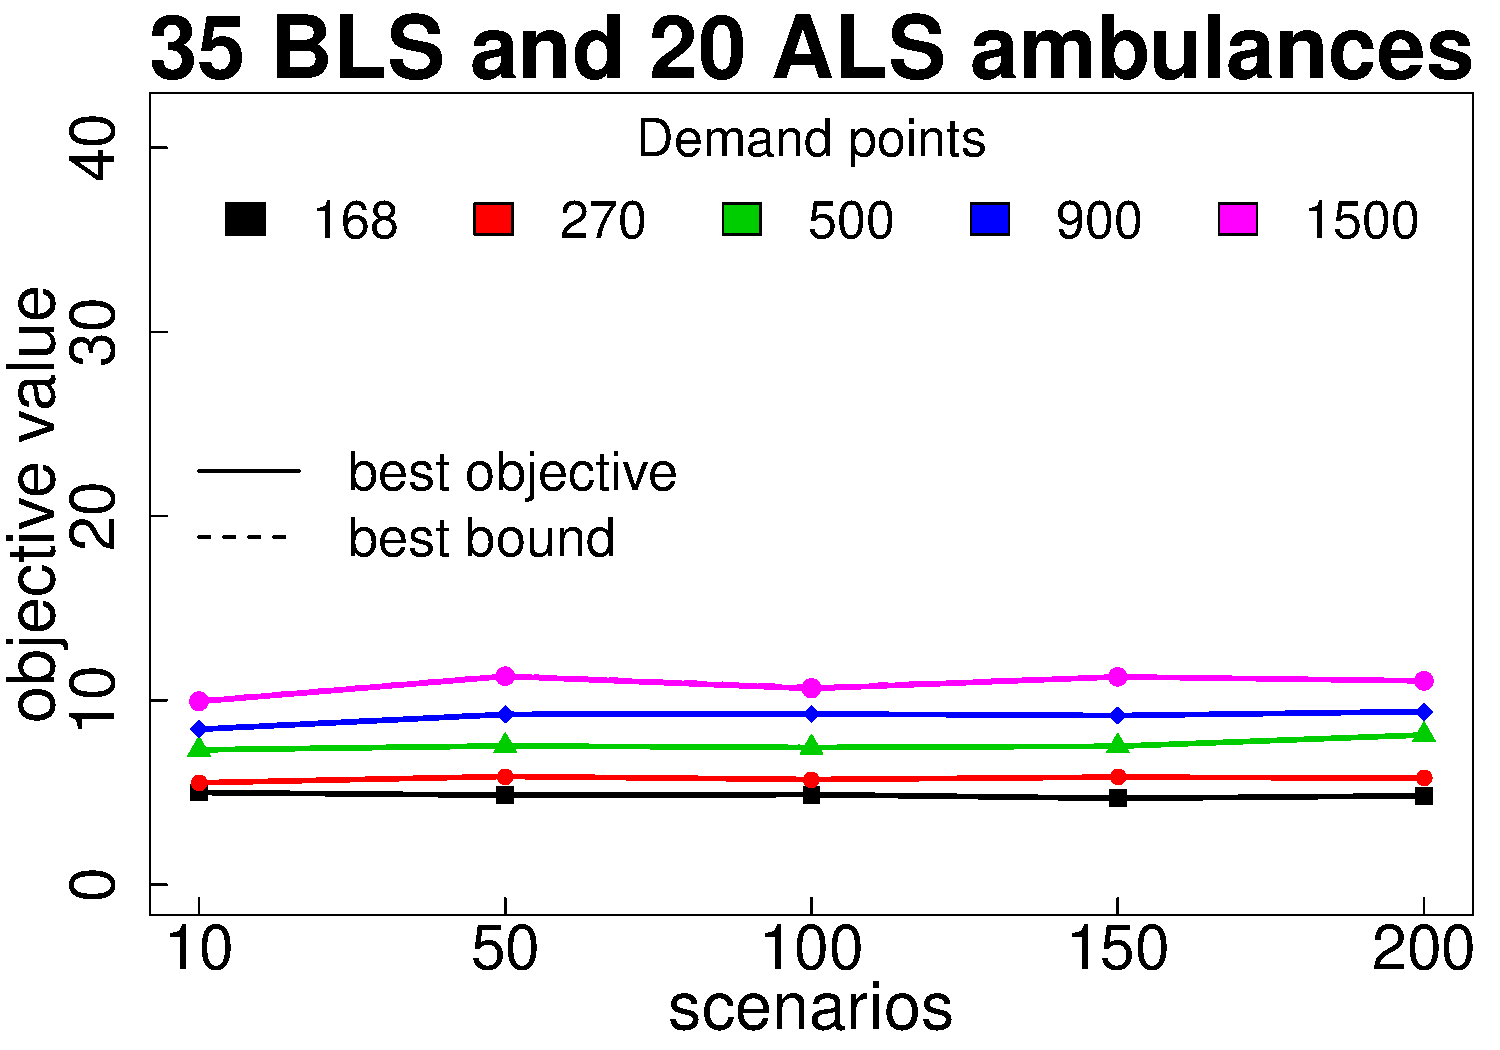
\includegraphics[width=0.42\textwidth]{Imagenes_Tesis/Math/Obj_Math_16_1.pdf}}{$|L|=16$}
\stackunder[4pt]{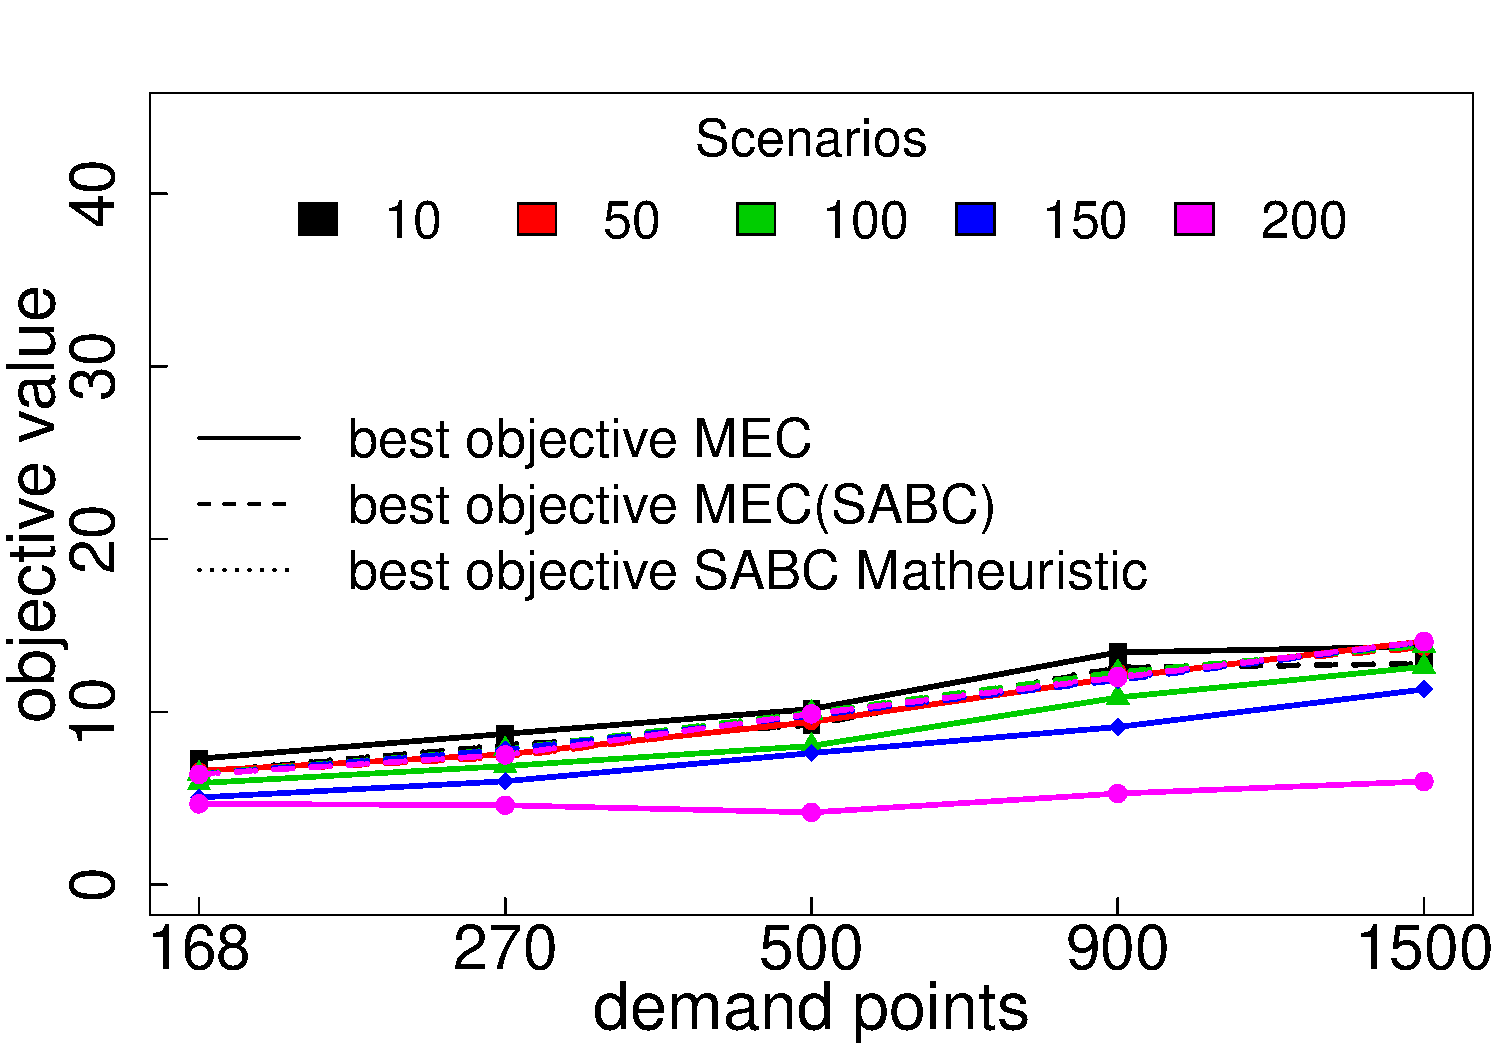
\includegraphics[width=0.42\textwidth]{Imagenes_Tesis/Math/Obj_Math_50.pdf}}{$|L|=50$}%
\hspace{0.4cm}%
\vspace{0.4cm}
\stackunder[4pt]{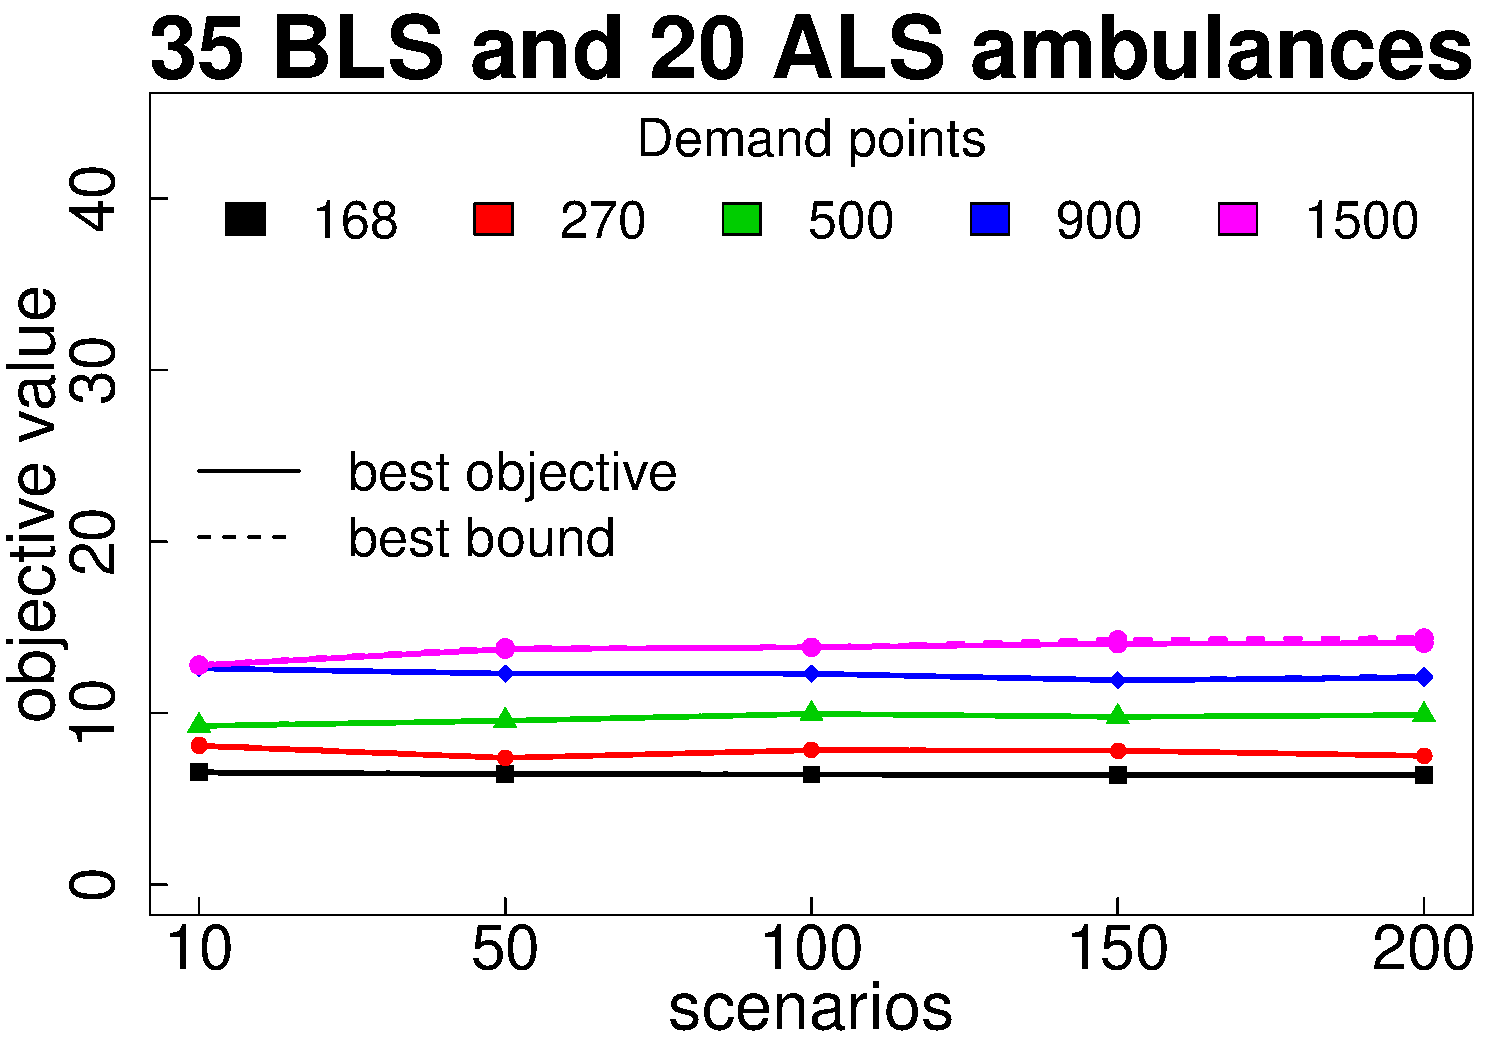
\includegraphics[width=0.42\textwidth]{Imagenes_Tesis/Math/Obj_Math_50_1.pdf}}{$|L|=50$}
\stackunder[4pt]{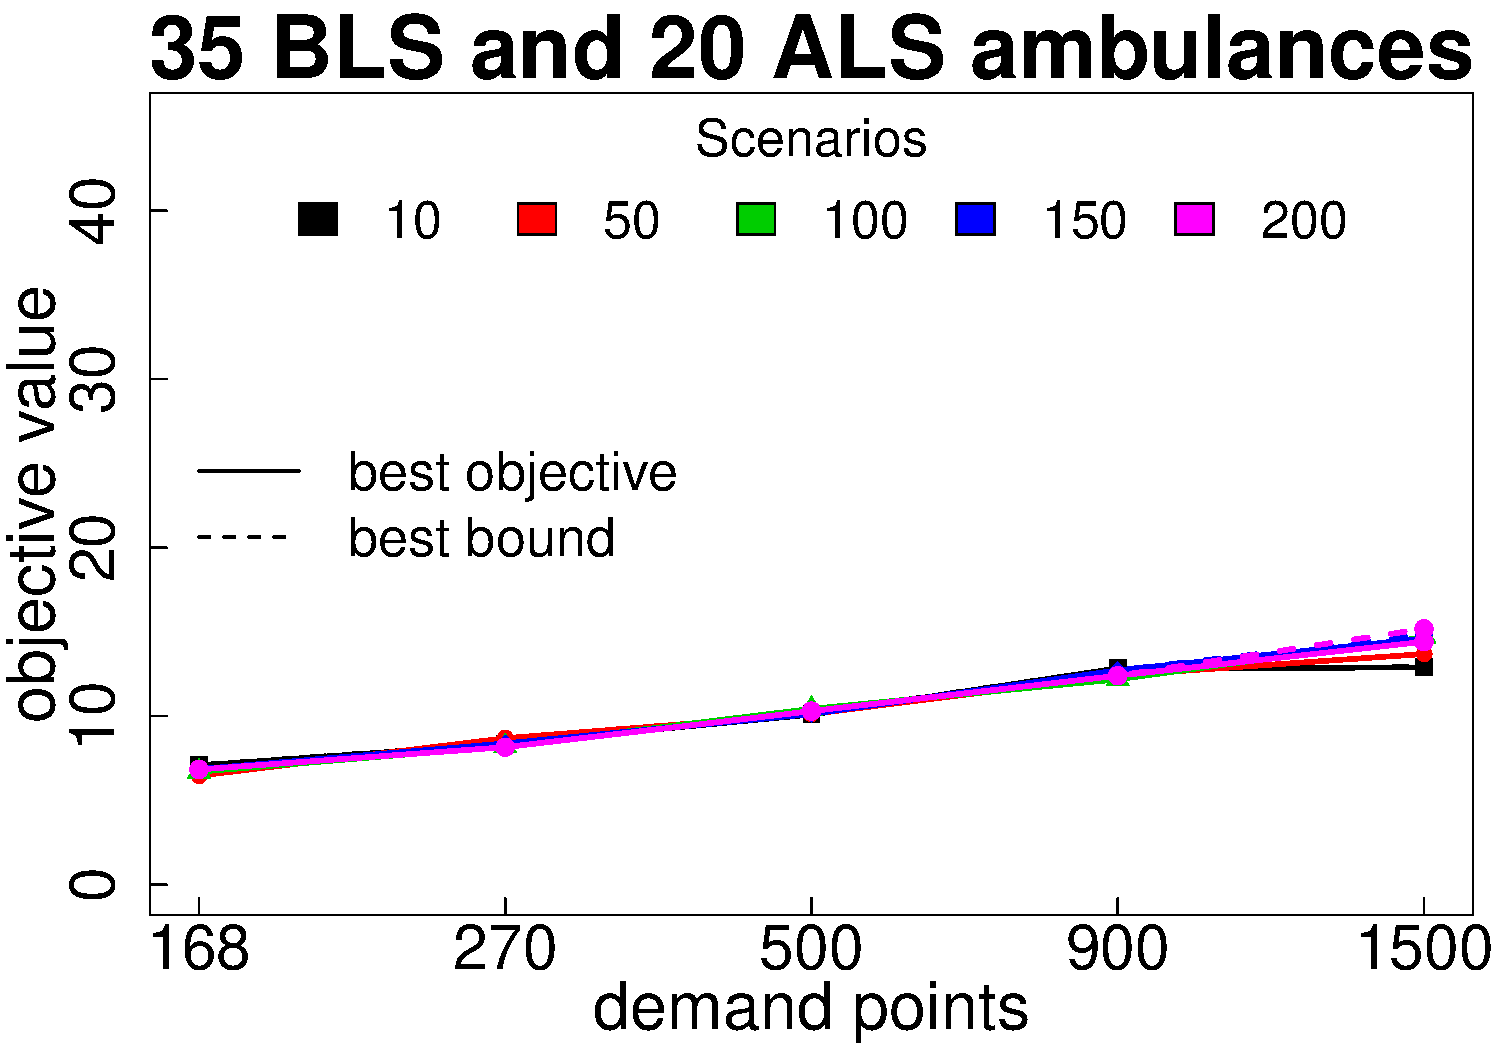
\includegraphics[width=0.42\textwidth]{Imagenes_Tesis/Math/Obj_Math_100.pdf}}{$|L|=100$}%
\hspace{0.4cm}%
\vspace{0.4cm}
\stackunder[4pt]{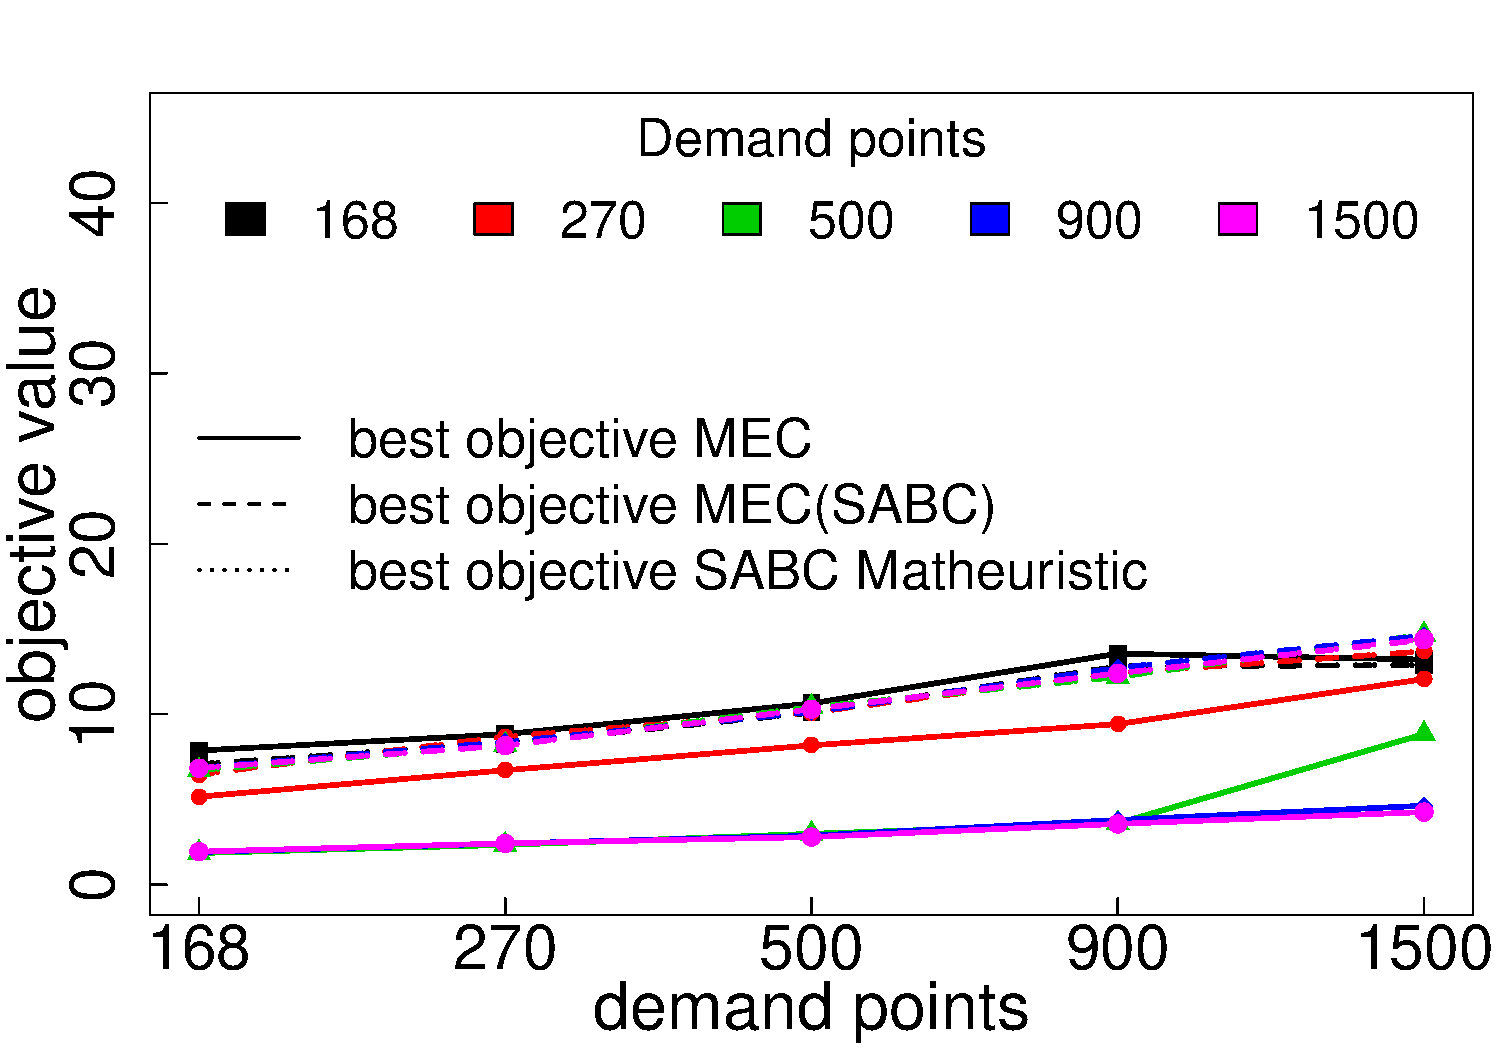
\includegraphics[width=0.42\textwidth]{Imagenes_Tesis/Math/Obj_Math_100_1.pdf}}{$|L|=100$}
\caption{Objective values of SABC Matheuristic.}
\label{Obj_Math}
\end{figure}


To see if the Matheuristic shows better results than MEC and MEC(SABC) methodology we compare the results between the objective values obtained from three of them. Figure \ref{Obj_Comp} shows these results. MEC objective values are represented for the straight lines and we can see that the other two types of lines, the dotted and the dashed ones, have better solutions than the straight line. Nonetheless, there is not a significant difference between MEC(SABC) and SABC Matheuristic. This small improvement may be due to the computational limit time the solver had to solve each instance. Although, we can see the improvement percentage between the MEC and the MEC(SABC) in column five of the Table \ref{table:objval}, and the improvement percentage between the MEC(SABC) and the SABC Matheuristic in column six. Column one define the instance name, which is given by the number of demand points, potential sites and scenarios. And columns two three and four have the objective values for the MEC, the MEC(SABC) and the SABC MAtheuristic respectively. Something interesting is that SABC Matheuristic mostly improves MEC solution for those instances where MEC(SABC) not improves the objective value. Table \ref{table:objval} shows only those instances where we obtain an improvement for the optimal solution. 


\begin{figure}[H]
\centering
\footnotesize
\stackunder[4pt]{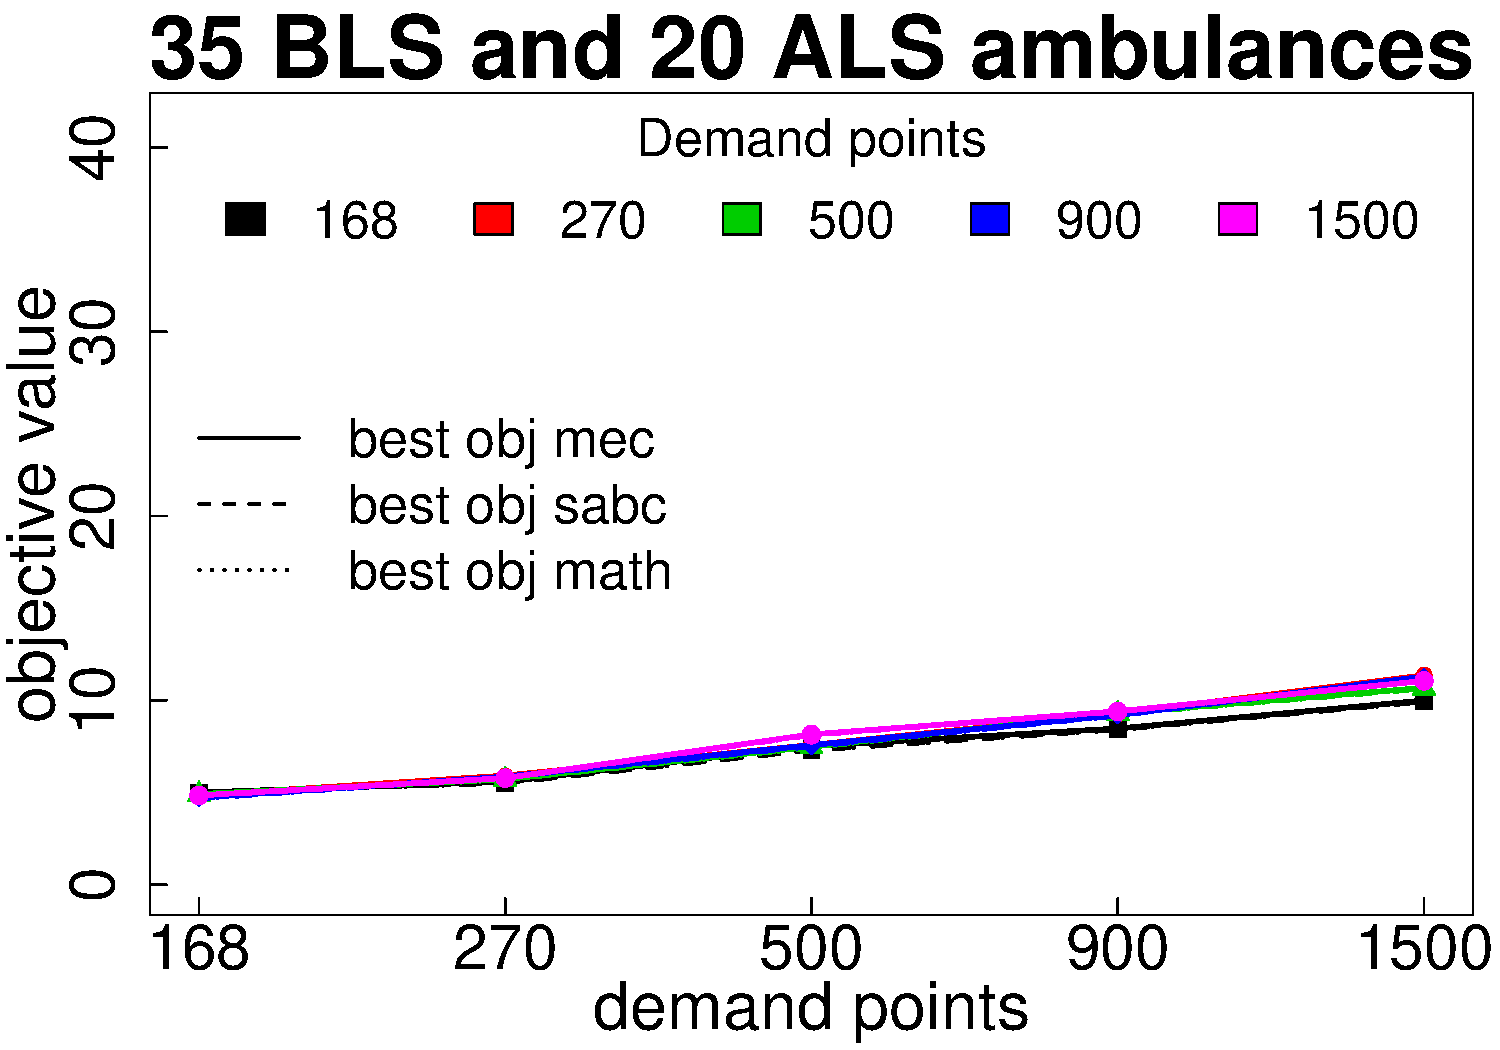
\includegraphics[width=0.42\textwidth]{Imagenes_Tesis/Comp/Obj_Comp_16.pdf}}{$|L|=16$}%
\hspace{0.4cm}%
\vspace{0.4cm}
\stackunder[4pt]{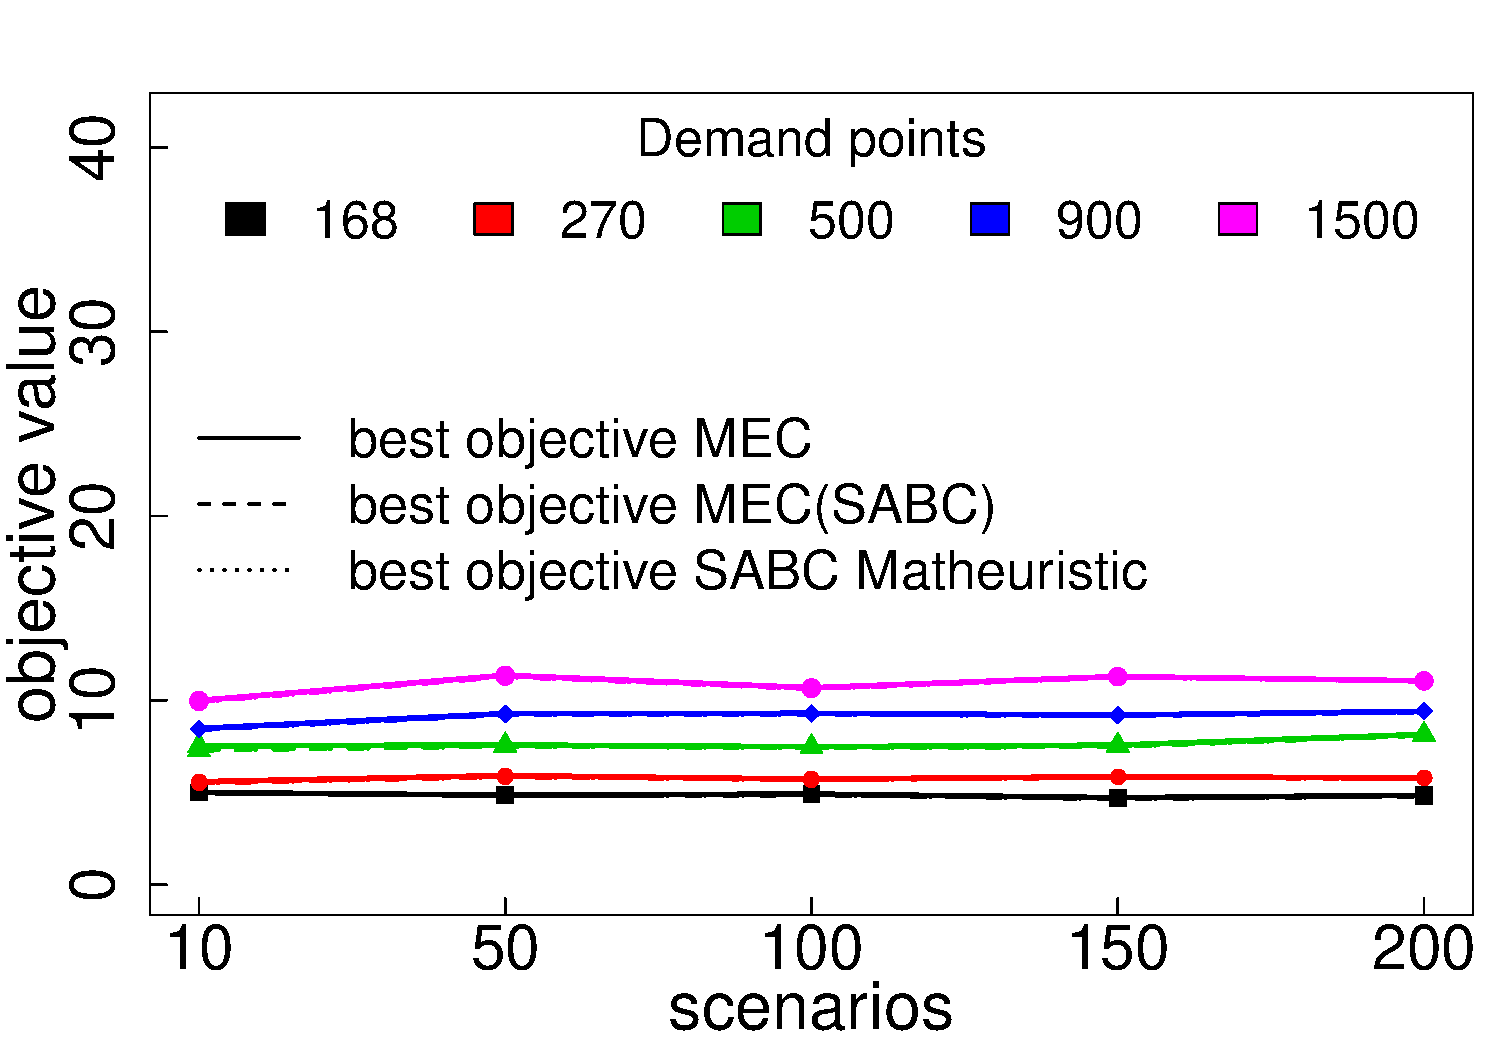
\includegraphics[width=0.42\textwidth]{Imagenes_Tesis/Comp/Obj_Comp_16_1.pdf}}{$|L|=16$}
\stackunder[4pt]{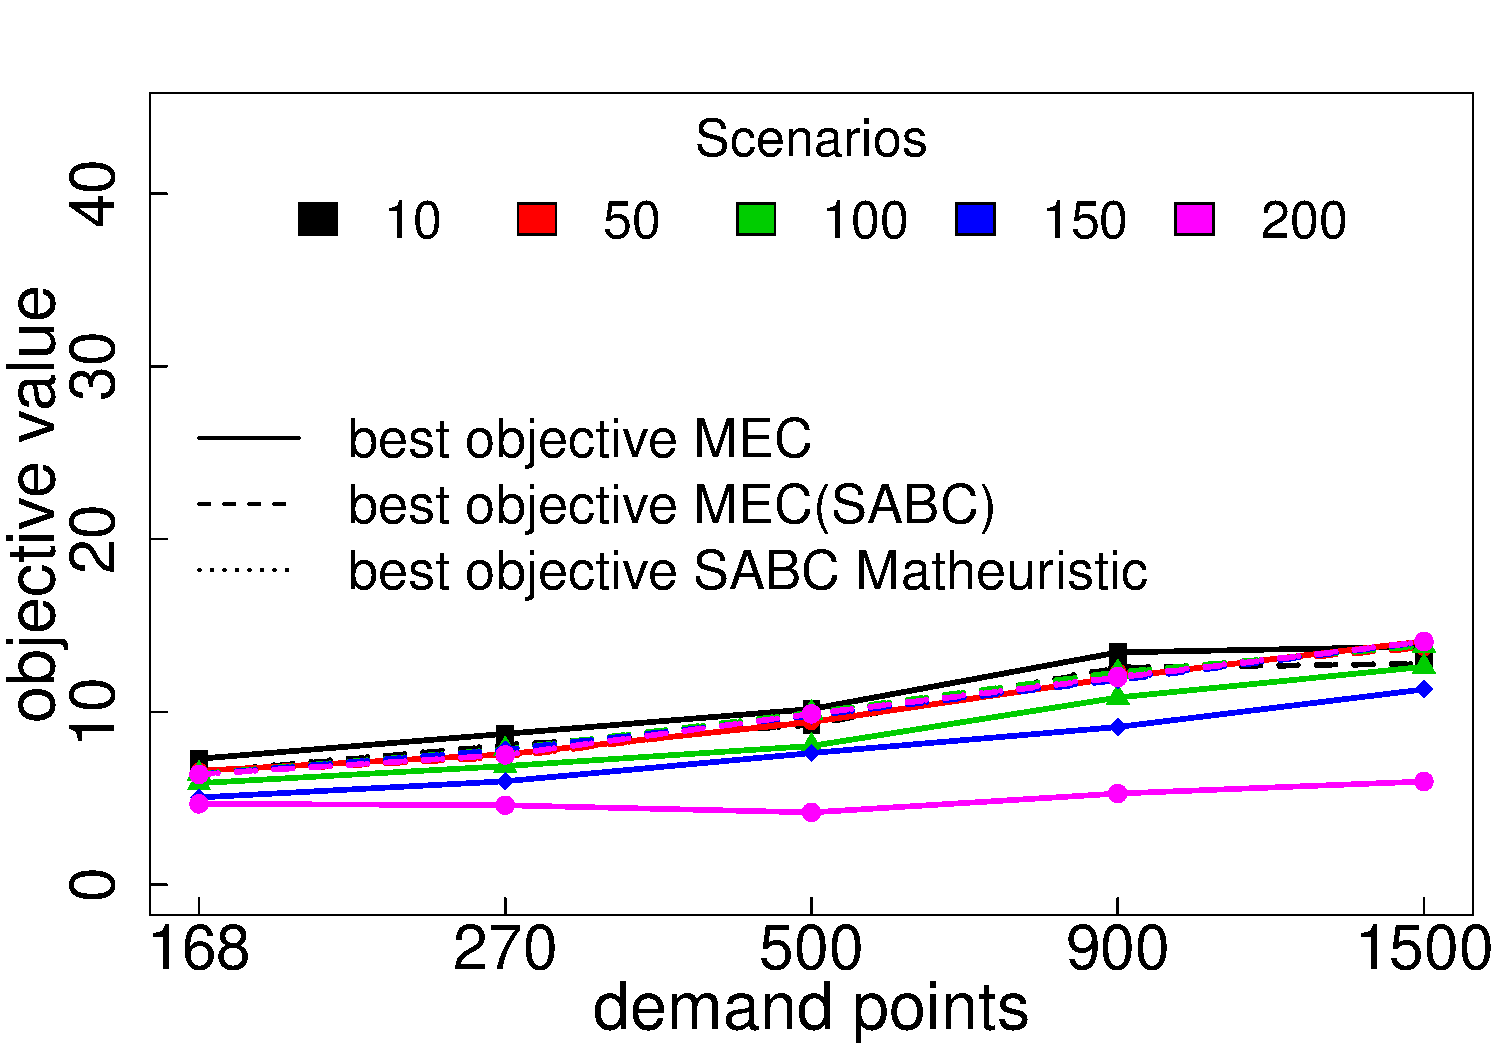
\includegraphics[width=0.42\textwidth]{Imagenes_Tesis/Comp/Obj_Comp_50.pdf}}{$|L|=50$}%
\hspace{0.4cm}%
\vspace{0.4cm}
\stackunder[4pt]{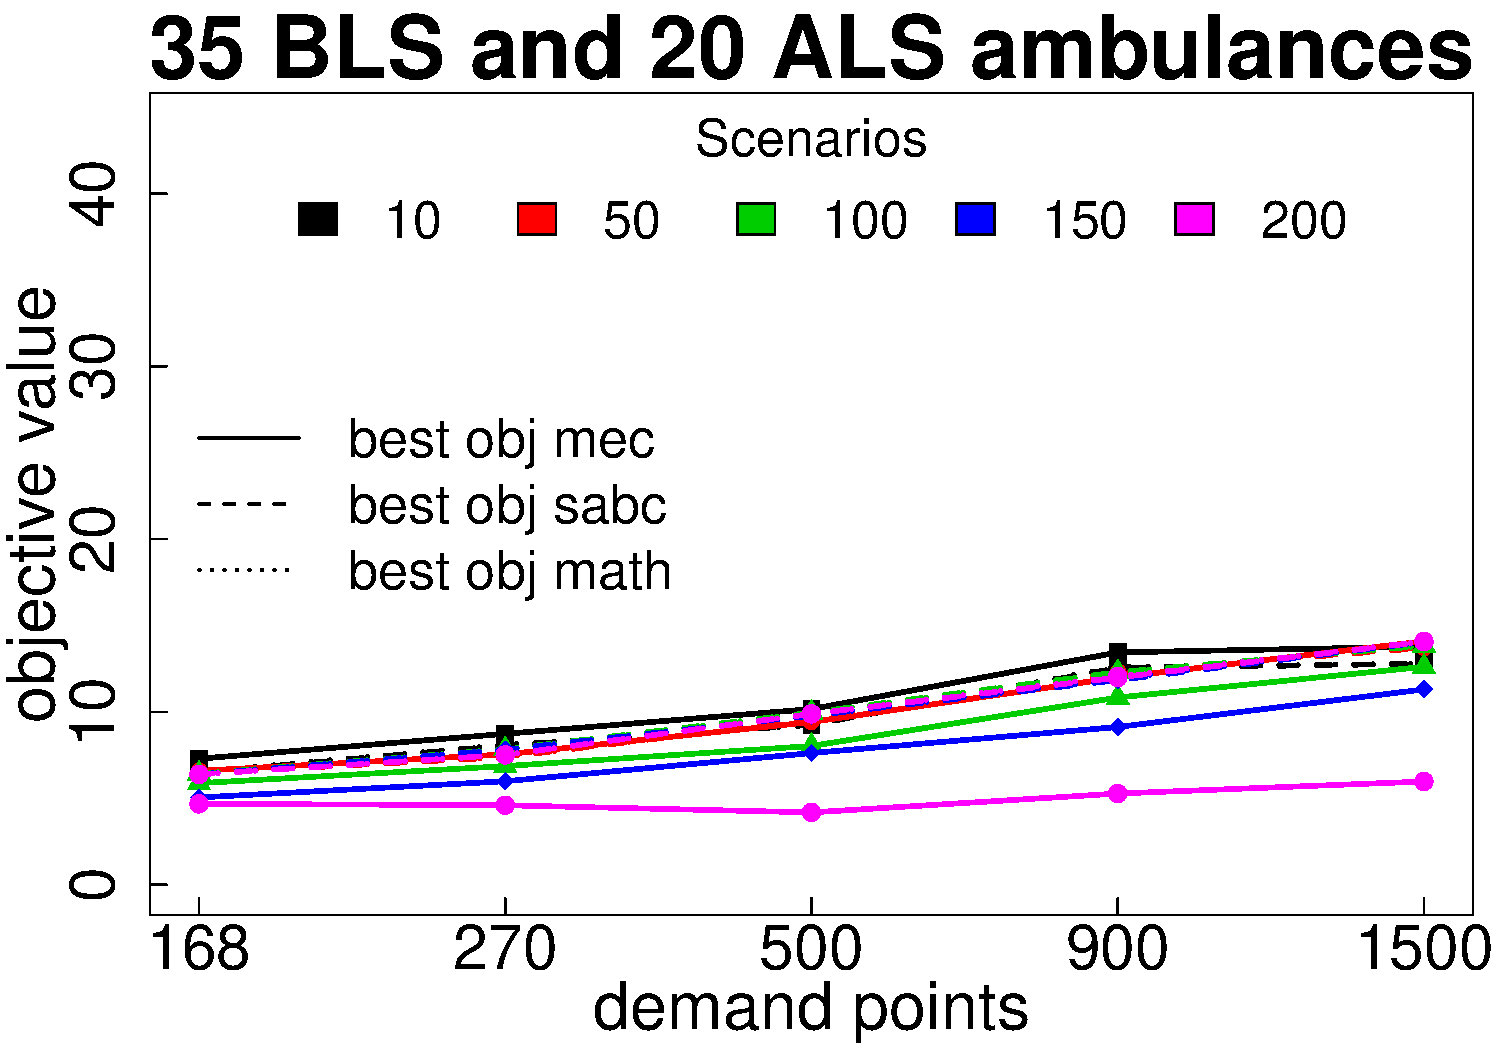
\includegraphics[width=0.42\textwidth]{Imagenes_Tesis/Comp/Obj_Comp_50_1.pdf}}{$|L|=50$}
\stackunder[4pt]{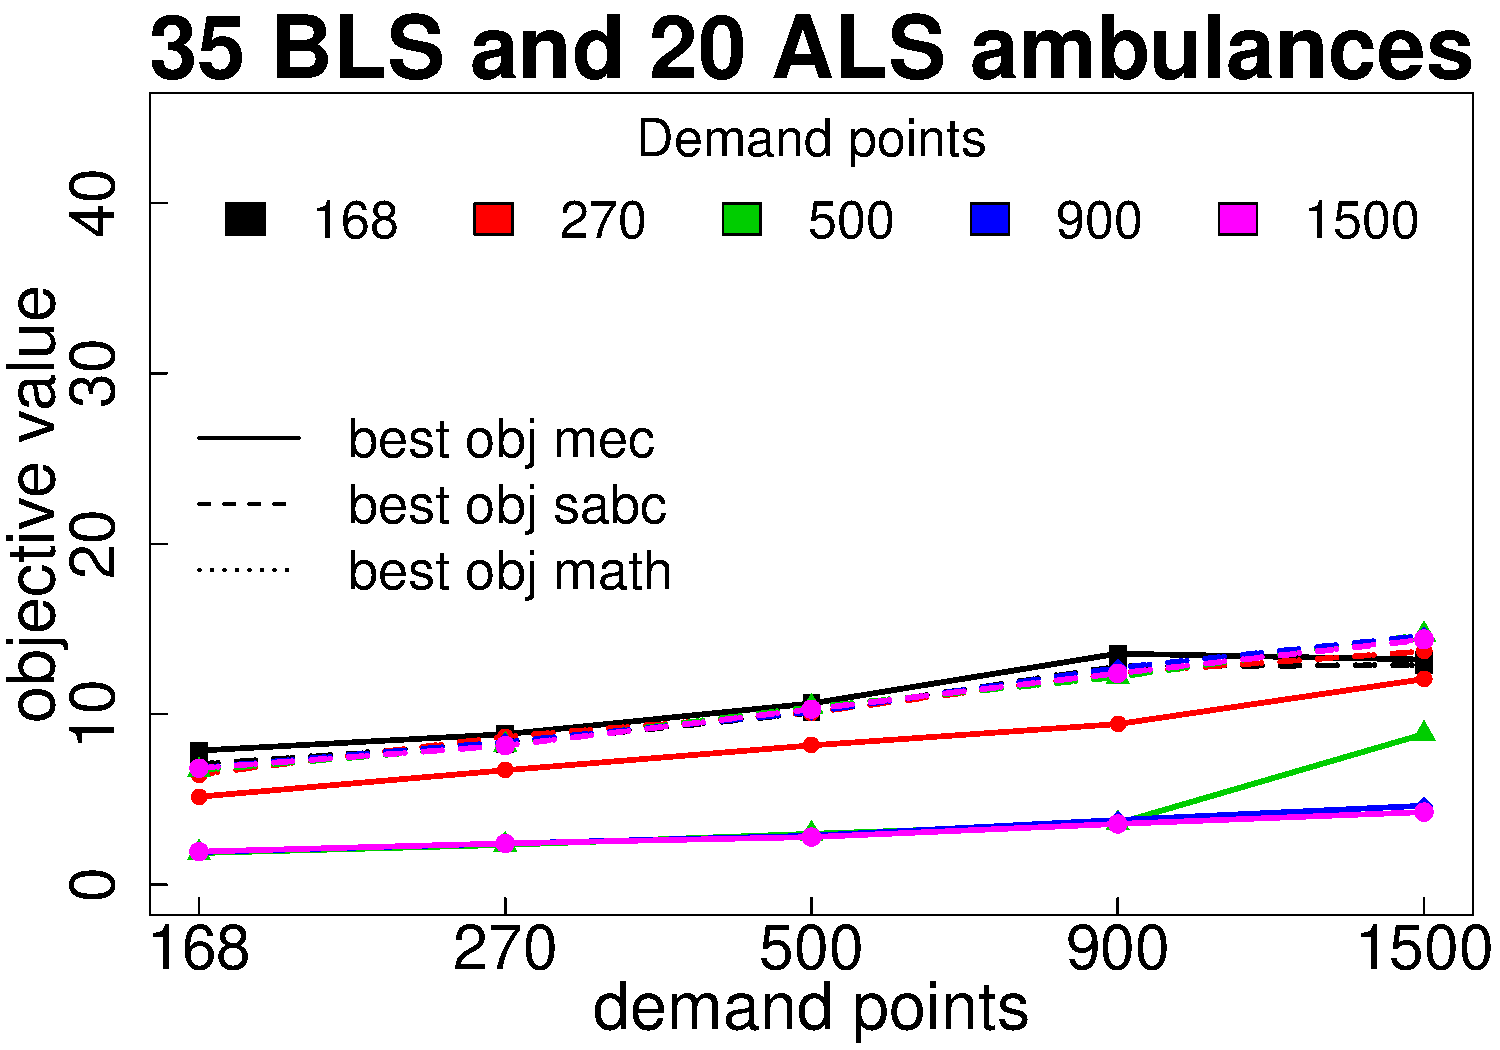
\includegraphics[width=0.42\textwidth]{Imagenes_Tesis/Comp/Obj_Comp_100.pdf}}{$|L|=100$}%
\hspace{0.4cm}%
\vspace{0.4cm}
\stackunder[4pt]{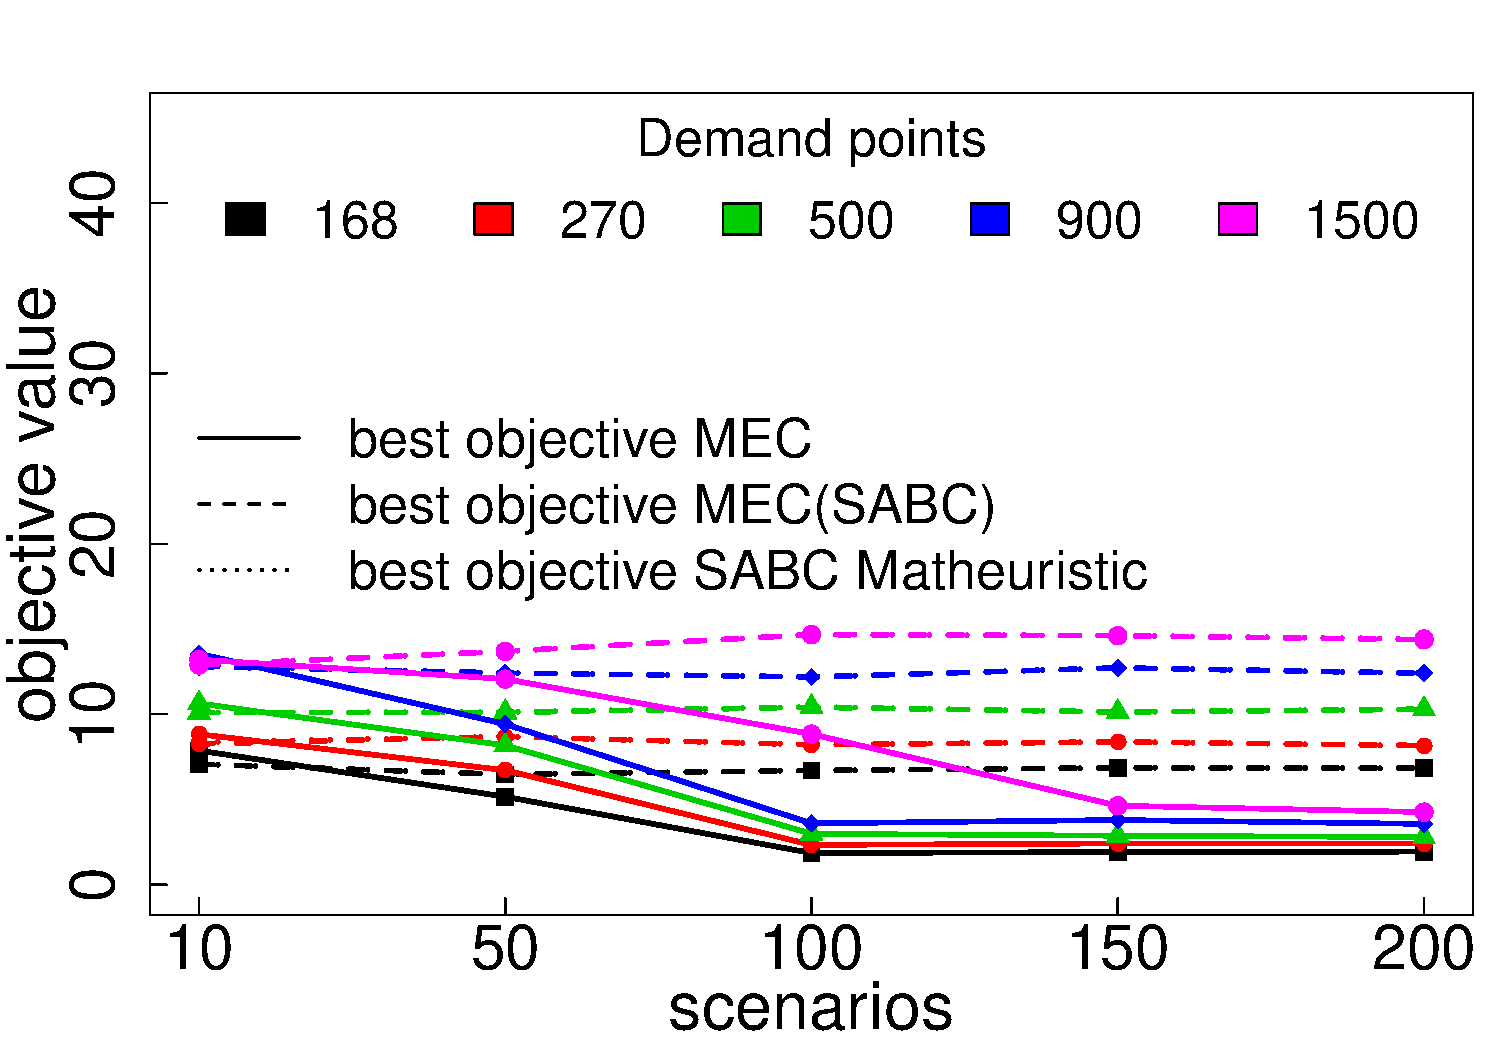
\includegraphics[width=0.42\textwidth]{Imagenes_Tesis/Comp/Obj_Comp_100_1.pdf}}{$|L|=100$}
\caption{Objective Comp.}
\label{Obj_Comp}
\end{figure}


% \usepackage{tabularray}
\begin{small}
\begin{longtblr}[
  caption = {Objective Values Comparison},
]{
  row{1} = {c},
  row{2} = {c},
  cell{1}{1} = {c=6}{},
  cell{3}{2} = {c},
  cell{3}{3} = {c},
  cell{3}{4} = {c},
  cell{3}{5} = {c},
  cell{3}{6} = {c},
  cell{4}{2} = {c},
  cell{4}{3} = {c},
  cell{4}{4} = {c},
  cell{4}{5} = {c},
  cell{4}{6} = {c},
  cell{5}{2} = {c},
  cell{5}{3} = {c},
  cell{5}{4} = {c},
  cell{5}{5} = {c},
  cell{5}{6} = {c},
  cell{6}{2} = {c},
  cell{6}{3} = {c},
  cell{6}{4} = {c},
  cell{6}{5} = {c},
  cell{6}{6} = {c},
  cell{7}{2} = {c},
  cell{7}{3} = {c},
  cell{7}{4} = {c},
  cell{7}{5} = {c},
  cell{7}{6} = {c},
  cell{8}{2} = {c},
  cell{8}{3} = {c},
  cell{8}{4} = {c},
  cell{8}{5} = {c},
  cell{8}{6} = {c},
  cell{9}{2} = {c},
  cell{9}{3} = {c},
  cell{9}{4} = {c},
  cell{9}{5} = {c},
  cell{9}{6} = {c},
  cell{10}{2} = {c},
  cell{10}{3} = {c},
  cell{10}{4} = {c},
  cell{10}{5} = {c},
  cell{10}{6} = {c},
  cell{11}{2} = {c},
  cell{11}{3} = {c},
  cell{11}{4} = {c},
  cell{11}{5} = {c},
  cell{11}{6} = {c},
  cell{12}{2} = {c},
  cell{12}{3} = {c},
  cell{12}{4} = {c},
  cell{12}{5} = {c},
  cell{12}{6} = {c},
  cell{13}{2} = {c},
  cell{13}{3} = {c},
  cell{13}{4} = {c},
  cell{13}{5} = {c},
  cell{13}{6} = {c},
  cell{14}{2} = {c},
  cell{14}{3} = {c},
  cell{14}{4} = {c},
  cell{14}{5} = {c},
  cell{14}{6} = {c},
  cell{15}{2} = {c},
  cell{15}{3} = {c},
  cell{15}{4} = {c},
  cell{15}{5} = {c},
  cell{15}{6} = {c},
  cell{16}{2} = {c},
  cell{16}{3} = {c},
  cell{16}{4} = {c},
  cell{16}{5} = {c},
  cell{16}{6} = {c},
  cell{17}{2} = {c},
  cell{17}{3} = {c},
  cell{17}{4} = {c},
  cell{17}{5} = {c},
  cell{17}{6} = {c},
  cell{18}{2} = {c},
  cell{18}{3} = {c},
  cell{18}{4} = {c},
  cell{18}{5} = {c},
  cell{18}{6} = {c},
  cell{19}{2} = {c},
  cell{19}{3} = {c},
  cell{19}{4} = {c},
  cell{19}{5} = {c},
  cell{19}{6} = {c},
  cell{20}{2} = {c},
  cell{20}{3} = {c},
  cell{20}{4} = {c},
  cell{20}{5} = {c},
  cell{20}{6} = {c},
  cell{21}{2} = {c},
  cell{21}{3} = {c},
  cell{21}{4} = {c},
  cell{21}{5} = {c},
  cell{21}{6} = {c},
  cell{22}{2} = {c},
  cell{22}{3} = {c},
  cell{22}{4} = {c},
  cell{22}{5} = {c},
  cell{22}{6} = {c},
  cell{23}{2} = {c},
  cell{23}{3} = {c},
  cell{23}{4} = {c},
  cell{23}{5} = {c},
  cell{23}{6} = {c},
  cell{24}{2} = {c},
  cell{24}{3} = {c},
  cell{24}{4} = {c},
  cell{24}{5} = {c},
  cell{24}{6} = {c},
  cell{25}{2} = {c},
  cell{25}{3} = {c},
  cell{25}{4} = {c},
  cell{25}{5} = {c},
  cell{25}{6} = {c},
  cell{26}{2} = {c},
  cell{26}{3} = {c},
  cell{26}{4} = {c},
  cell{26}{5} = {c},
  cell{26}{6} = {c},
  cell{27}{2} = {c},
  cell{27}{3} = {c},
  cell{27}{4} = {c},
  cell{27}{5} = {c},
  cell{27}{6} = {c},
  cell{28}{2} = {c},
  cell{28}{3} = {c},
  cell{28}{4} = {c},
  cell{28}{5} = {c},
  cell{28}{6} = {c},
  cell{29}{2} = {c},
  cell{29}{3} = {c},
  cell{29}{4} = {c},
  cell{29}{5} = {c},
  cell{29}{6} = {c},
  cell{30}{2} = {c},
  cell{30}{3} = {c},
  cell{30}{4} = {c},
  cell{30}{5} = {c},
  cell{30}{6} = {c},
  cell{31}{2} = {c},
  cell{31}{3} = {c},
  cell{31}{4} = {c},
  cell{31}{5} = {c},
  cell{31}{6} = {c},
  cell{32}{2} = {c},
  cell{32}{3} = {c},
  cell{32}{4} = {c},
  cell{32}{5} = {c},
  cell{32}{6} = {c},
  cell{33}{2} = {c},
  cell{33}{3} = {c},
  cell{33}{4} = {c},
  cell{33}{5} = {c},
  cell{33}{6} = {c},
  cell{34}{2} = {c},
  cell{34}{3} = {c},
  cell{34}{4} = {c},
  cell{34}{5} = {c},
  cell{34}{6} = {c},
  cell{35}{2} = {c},
  cell{35}{3} = {c},
  cell{35}{4} = {c},
  cell{35}{5} = {c},
  cell{35}{6} = {c},
  cell{36}{2} = {c},
  cell{36}{3} = {c},
  cell{36}{4} = {c},
  cell{36}{5} = {c},
  cell{36}{6} = {c},
  cell{37}{2} = {c},
  cell{37}{3} = {c},
  cell{37}{4} = {c},
  cell{37}{5} = {c},
  cell{37}{6} = {c},
  cell{38}{2} = {c},
  cell{38}{3} = {c},
  cell{38}{4} = {c},
  cell{38}{5} = {c},
  cell{38}{6} = {c},
  cell{39}{2} = {c},
  cell{39}{3} = {c},
  cell{39}{4} = {c},
  cell{39}{5} = {c},
  cell{39}{6} = {c},
  cell{40}{2} = {c},
  cell{40}{3} = {c},
  cell{40}{4} = {c},
  cell{40}{5} = {c},
  cell{40}{6} = {c},
  cell{41}{2} = {c},
  cell{41}{3} = {c},
  cell{41}{4} = {c},
  cell{41}{5} = {c},
  cell{41}{6} = {c},
  cell{42}{2} = {c},
  cell{42}{3} = {c},
  cell{42}{4} = {c},
  cell{42}{5} = {c},
  cell{42}{6} = {c},
  cell{43}{2} = {c},
  cell{43}{3} = {c},
  cell{43}{4} = {c},
  cell{43}{5} = {c},
  cell{43}{6} = {c},
  cell{44}{2} = {c},
  cell{44}{3} = {c},
  cell{44}{4} = {c},
  cell{44}{5} = {c},
  cell{44}{6} = {c},
  cell{45}{2} = {c},
  cell{45}{3} = {c},
  cell{45}{4} = {c},
  cell{45}{5} = {c},
  cell{45}{6} = {c},
  cell{46}{2} = {c},
  cell{46}{3} = {c},
  cell{46}{4} = {c},
  cell{46}{5} = {c},
  cell{46}{6} = {c},
  cell{47}{2} = {c},
  cell{47}{3} = {c},
  cell{47}{4} = {c},
  cell{47}{5} = {c},
  cell{47}{6} = {c},
  cell{48}{2} = {c},
  cell{48}{3} = {c},
  cell{48}{4} = {c},
  cell{48}{5} = {c},
  cell{48}{6} = {c},
  cell{49}{2} = {c},
  cell{49}{3} = {c},
  cell{49}{4} = {c},
  cell{49}{5} = {c},
  cell{49}{6} = {c},
  cell{50}{2} = {c},
  cell{50}{3} = {c},
  cell{50}{4} = {c},
  cell{50}{5} = {c},
  cell{50}{6} = {c},
  cell{51}{2} = {c},
  cell{51}{3} = {c},
  cell{51}{4} = {c},
  cell{51}{5} = {c},
  cell{51}{6} = {c},
  cell{52}{2} = {c},
  cell{52}{3} = {c},
  cell{52}{4} = {c},
  cell{52}{5} = {c},
  cell{52}{6} = {c},
  cell{53}{2} = {c},
  cell{53}{3} = {c},
  cell{53}{4} = {c},
  cell{53}{5} = {c},
  cell{53}{6} = {c},
  hlines,
  vlines,
}
Objective values~ &            &             &                        &                                  &                                   \\
{Instance \\ $|I|$ $|L|$ $|S|$}          & MEC        & MEC(SABC)   & {Matheuristic\\(Math)} & {\% Improve\\MEC vs \\MEC(SABC)} & {\% Improve\\MEC(SABC) \\vs Math} \\
1500 16 200       & 11.0536    & 11.05635    & 11.05635               & 0.024878773                      & -                                 \\
168 50 10         & 7.285      & 6.485       & 6.53                   & -                                & 0.693909021                       \\
168 50 100        & 5.86825    & 6.4167      & 6.4167                 & 9.346057172                      & -                                 \\
168 50 150        & 5.04052222 & 6.375988893 & 6.375988893            & 26.4946093                       & -                                 \\
168 50 200        & 4.6735     & 6.3773      & 6.3773                 & 36.4566171                       & -                                 \\
270 50 10         & 8.725      & 8.05        & 8.085                  & -                                & 0.434782609                       \\
270 50 50         & 7.535      & 7.381       & 7.389                  & -                                & 0.108386398                       \\
270 50 100        & 6.85685    & 7.83305     & 7.83305                & 14.23685803                      & -                                 \\
270 50 150        & 5.9789     & 7.80876667  & 7.80876667             & 30.60540685                      & -                                 \\
270 50 200        & 4.59045    & 7.504750002 & 7.504750002            & 63.48615064                      & -                                 \\
500 50 50         & 9.4105     & 9.547000009 & 9.547000009            & 1.450507504                      & -                                 \\
500 50 100        & 8.02305    & 9.9521      & 9.9521                 & 24.04384866                      & -                                 \\
500 50 150        & 7.61198889 & 9.7781      & 9.7781                 & 28.45657216                      & -                                 \\
500 50 200        & 4.17615    & 9.883800001 & 9.883800001            & 136.6725333                      & -                                 \\
900 50 10         & 13.4365    & 12.535      & 12.603                 & -                                & 0.542481053                       \\
900 50 50         & 11.987     & 12.286      & 12.301                 & 2.4943689                        & 0.122090184                       \\
900 50 100        & 10.8234    & 12.29315    & 12.29565               & 13.57937432                      & 0.020336529                       \\
900 50 150        & 9.11984444 & 11.83602222 & 11.91226667            & 29.78315908                      & 0.644172873                       \\
900 50 200        & 5.26805    & 11.98405    & 12.04855               & 127.4855022                      & 0.53821538                        \\
1500 50 50        & 14.084     & 13.709      & 13.7235                & -                                & 0.10576994                        \\
1500 50 100       & 12.6053    & 13.82855    & 13.82855               & 9.704251386                      & -                                 \\
1500 50 150       & 11.2970444 & 14.03975556 & 14.03975556            & 24.27812983                      & -                                 \\
1500 50 200       & 5.9664     & 14.0559     & 14.0723                & 135.5842719                      & 0.116676984                       \\
168 100 50        & 5.156      & 6.463000009 & 6.463000009            & 25.34910801                      & -                                 \\
168 100 100       & 1.8485     & 6.6976      & 6.6976                 & 262.3262105                      & -                                 \\
168 100 150       & 1.9081     & 6.85182223  & 6.85182223             & 259.0913594                      & -                                 \\
168 100 200       & 1.93335    & 6.8329      & 6.8329                 & 253.4228153                      & -                                 \\
270 100 10        & 8.82500001 & 8.255000064 & 8.355                  & -                                & 1.211386255                       \\
270 100 50        & 6.71       & 8.6855      & 8.6855                 & 29.44113264                      & -                                 \\
270 100 100       & 2.32665    & 8.208650004 & 8.208650004            & 252.8098341                      & -                                 \\
270 100 150       & 2.41097778 & 8.375244449 & 8.375244449            & 247.3795788                      & -                                 \\
270 100 200       & 2.4159     & 8.15665     & 8.15665                & 237.6236599                      & -                                 \\
500 100 50        & 8.169      & 10.101      & 10.124                 & 23.6503856                       & 0.22770023                        \\
500 100 100       & 2.97905    & 10.40835    & 10.4282                & 249.384871                       & 0.190712265                       \\
500 100 150       & 2.86453333 & 10.12661111 & 10.12661111            & 253.5169584                      & -                                 \\
500 100 200       & 2.78645    & 10.29585    & 10.29585               & 269.4970304                      & -                                 \\
900 100 10        & 13.5535    & 12.79       & 12.8315                & -                                & 0.324472244                       \\
900 100 50        & 9.42       & 12.4165     & 12.4165                & 31.80997877                      & -                                 \\
900 100 100       & 3.59       & 12.18375    & 12.18375               & 239.3802228                      & -                                 \\
900 100 150       & 3.78992222 & 12.71902222 & 12.71902222            & 235.6011411                      & -                                 \\
900 100 200       & 3.5589     & 12.4005     & 12.4005                & 248.4363146                      & -                                 \\
1500 100 10       & 13.206     & 12.887      & 12.889                 & -                                & 0.015519516                       \\
1500 100 50       & 12.063     & 13.6875     & 13.6875                & 13.4667993                       & -                                 \\
1500 100 100      & 8.8318     & 14.67245    & 14.67245               & 66.13204556                      & -                                 \\
1500 100 150      & 4.62758889 & 14.60712222 & 14.60712222            & 215.6529798                      & -                                 \\
1500 100 200      & 4.2533     & 14.3678     & 14.41435               & 237.8035878                      & 0.323988387                        
\label{table:objval}
\end{longtblr}
\end{small}


SABC Matheuristic depends on the time we allow for the neighborhoods exploration. As the number of demand points, potential sites and scenarios increases, the number of neighbors in each neighborhood also increases. Considering that each neighbor is verified for the MEC(SABC), the computational time required is very large if we let SABC Matheuristic doing a complete procedure. Although, we checked some instances increasing the computational time to 10800 seconds per neighbor. Results for a selected set are in Table \ref{table:moretime}, whose structure is similar to the previous table. In these result we can see that improvements are very small but we were able to get an improvement for instances where we didn't get improvements before. Even so, since these are small instances, the MEC is still better.


% \usepackage{tabularray}
\begin{longtblr}[
  caption = {Objective Values Comparison with more time},
]{
  row{1} = {c},
  column{even} = {c},
  column{3} = {c},
  column{5} = {c},
  cell{1}{1} = {c=6}{},
  hlines,
  vlines,
}
Objective values                                                                          &             &             &                      &                                  &                                         \\
{Instance\\ \textbar{}I\textbar{} \textbar{}L\textbar{} \textbar{}S\textbar{}} & MEC         & MEC(SABC)   & {Matheuristic\\Math} & {\% Improve\\MEC vs \\MEC(SABC)} & {\% Improve\\MEC(SABC)\\vs Math} \\
168 16 10                                                                                 & 4.995000008 & 4.995       & 4.995000016          &         -                         & 3.16983E-07                             \\
168 16 50                      -                                                          & 4.849       & 4.848       & 4.848000001          &         -                       & 1.43126E-08                             \\
168 16 100                     -                                                           & 4.91145     & 4.88345     & 4.887450001          &         -                        & 0,081909319                             \\
168 16 150                     -                                                          & 4.713244444 & 4.677400001 & 4.678066671          &         -                        & 0,014252984                             \\
168 16 200                     -                                                          & 4.84205     & 4.8221      & 4.82355              &         -                        & 0,030069887                             \\
168 50 10                      -                                                          & 7.285       & 6.485       & 6.540000002          &         -                        & 0,848111051                             \\
168 50 50                      -                                                          & 6.5825      & 6.441       & 6.464                &         -                         & 0,357087409                             \\
168 50 100                                                                                & 5.86825     & 6.4167      & 6.4623               & 9.346057172                      & 0,710645659                             \\
168 50 150                                                                                & 5.040522223 & 6.375988893 & 6.417422223          & 26.4946093                       & 0,649833788                             \\
168 50 200                                                                                & 4.6735      & 6.3773      & 6.4149               & 36.4566171                       & 0,589591206                             \\
168 100 10                                                                                & 7.865       & 7.070000095 & 7.18                 &         -                        & 1.555868511                             \\
168 100 50                                                                                & 5.156       & 6.463000009 & 6.513                & 25.34910801                      & 0,773634398                             \\
168 100 100                                                                               & 1.8485      & 6.6976      & 6.717600001          & 262.3262105                      & 0,298614435                             \\
168 100 150                                                                               & 1.9081      & 6.85182223  & 6.8787               & 259.0913594                      & 0,392271858                             \\
168 100 200                                                                               & 1.93335     & 6.8329      & 6.8721               & 253.4228153                      & 0,573694917                             \\
270 16 10                                                                                 & 5.580000003 & 5.525       & 5.535                &       -                           & 0,180995475                             \\
270 16 50                                                                                 & 5.9145      & 5.8675      & 5.872500001          &       -                           & 0,085215177                             \\
270 16 100                                                                                & 5.719       & 5.70245     & 5.70465              &       -                           & 0,038579906                             \\
270 16 150                                                                                & 5.857844447 & 5.834588893 & 5.835666673          &       -                           & 0,018472238                             \\
270 16 200                                                                                & 5.7808      & 5.77065     & 5.771                &       -                           & 0,006065175                             
\label{table:moretime}
\end{longtblr}

%\begin{figure}[H]
%\centering
%\footnotesize
%\stackunder[4pt]{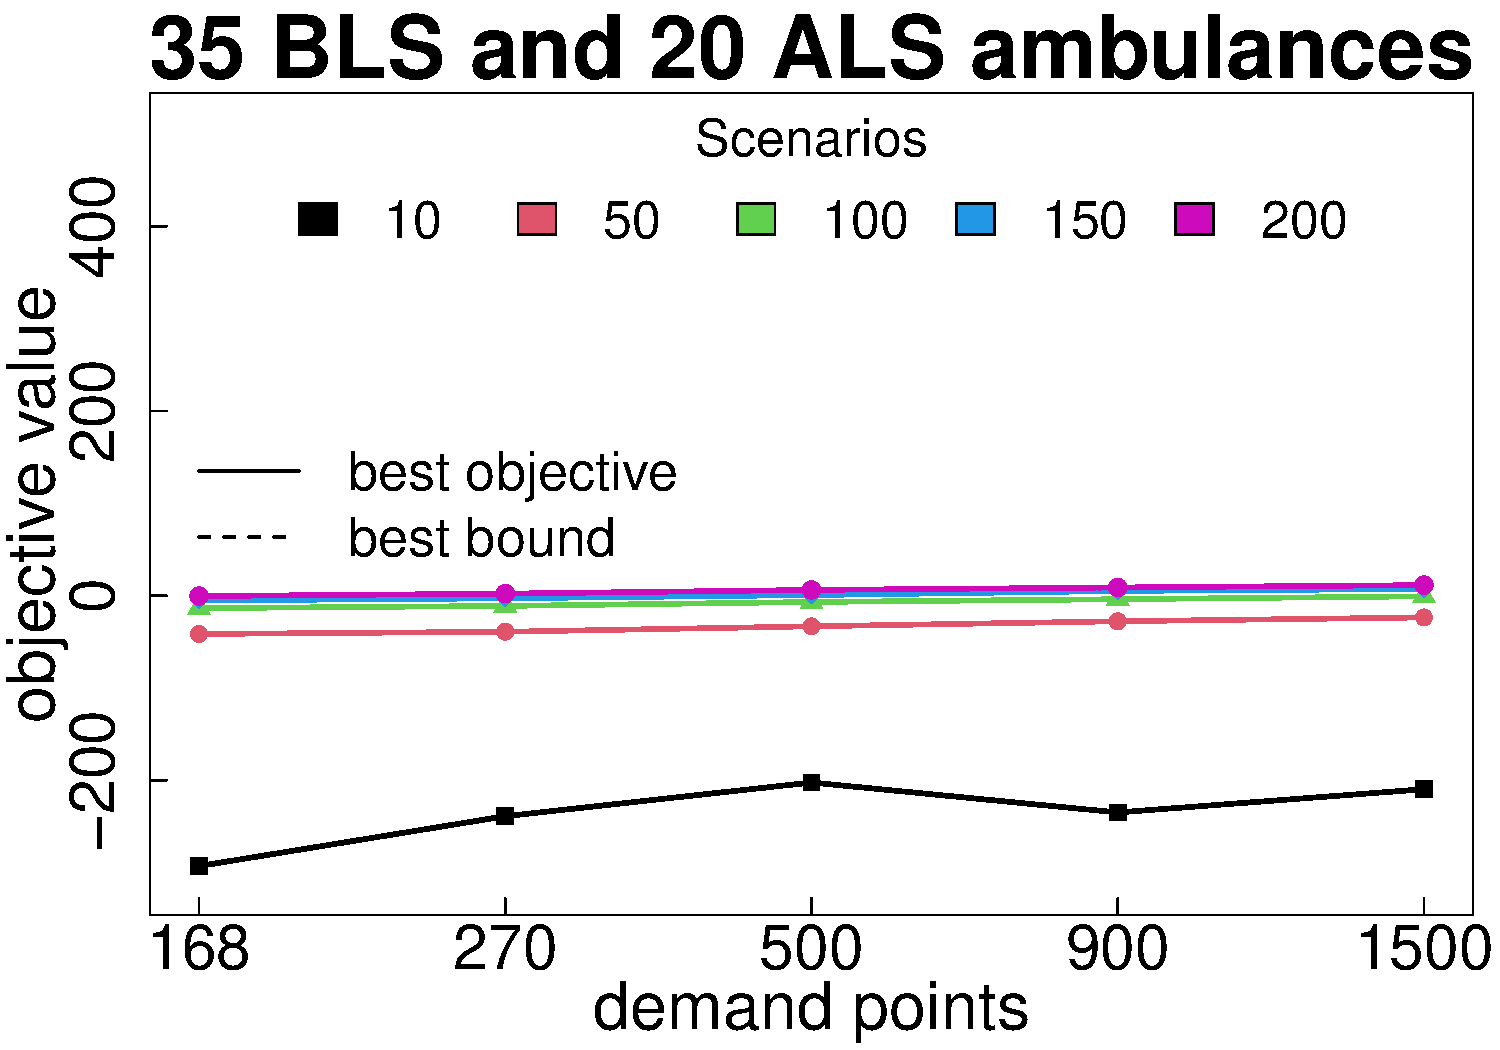
\includegraphics[width=0.42\textwidth]{Imagenes_Tesis/SABC/Obj_SABC_16.pdf}}{$|L|=16$}%
%\hspace{0.4cm}%
%\vspace{0.4cm}
%\stackunder[4pt]{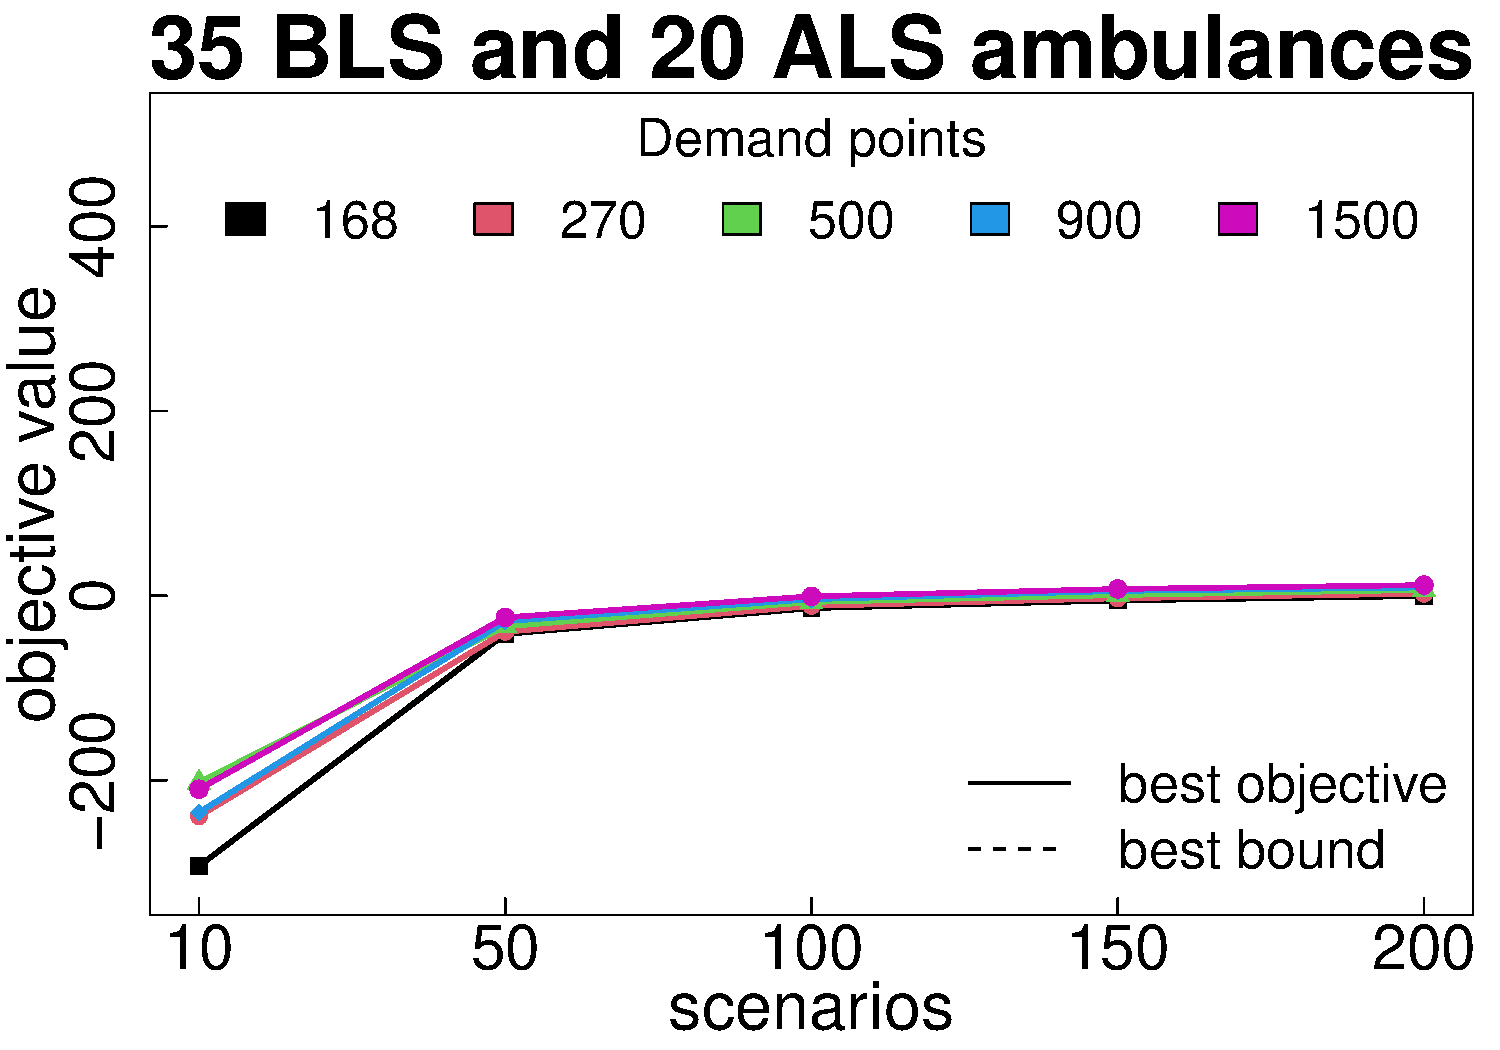
\includegraphics[width=0.42\textwidth]{Imagenes_Tesis/SABC/Obj_SABC_16_1.pdf}}{$|L|=16$}
%\stackunder[4pt]{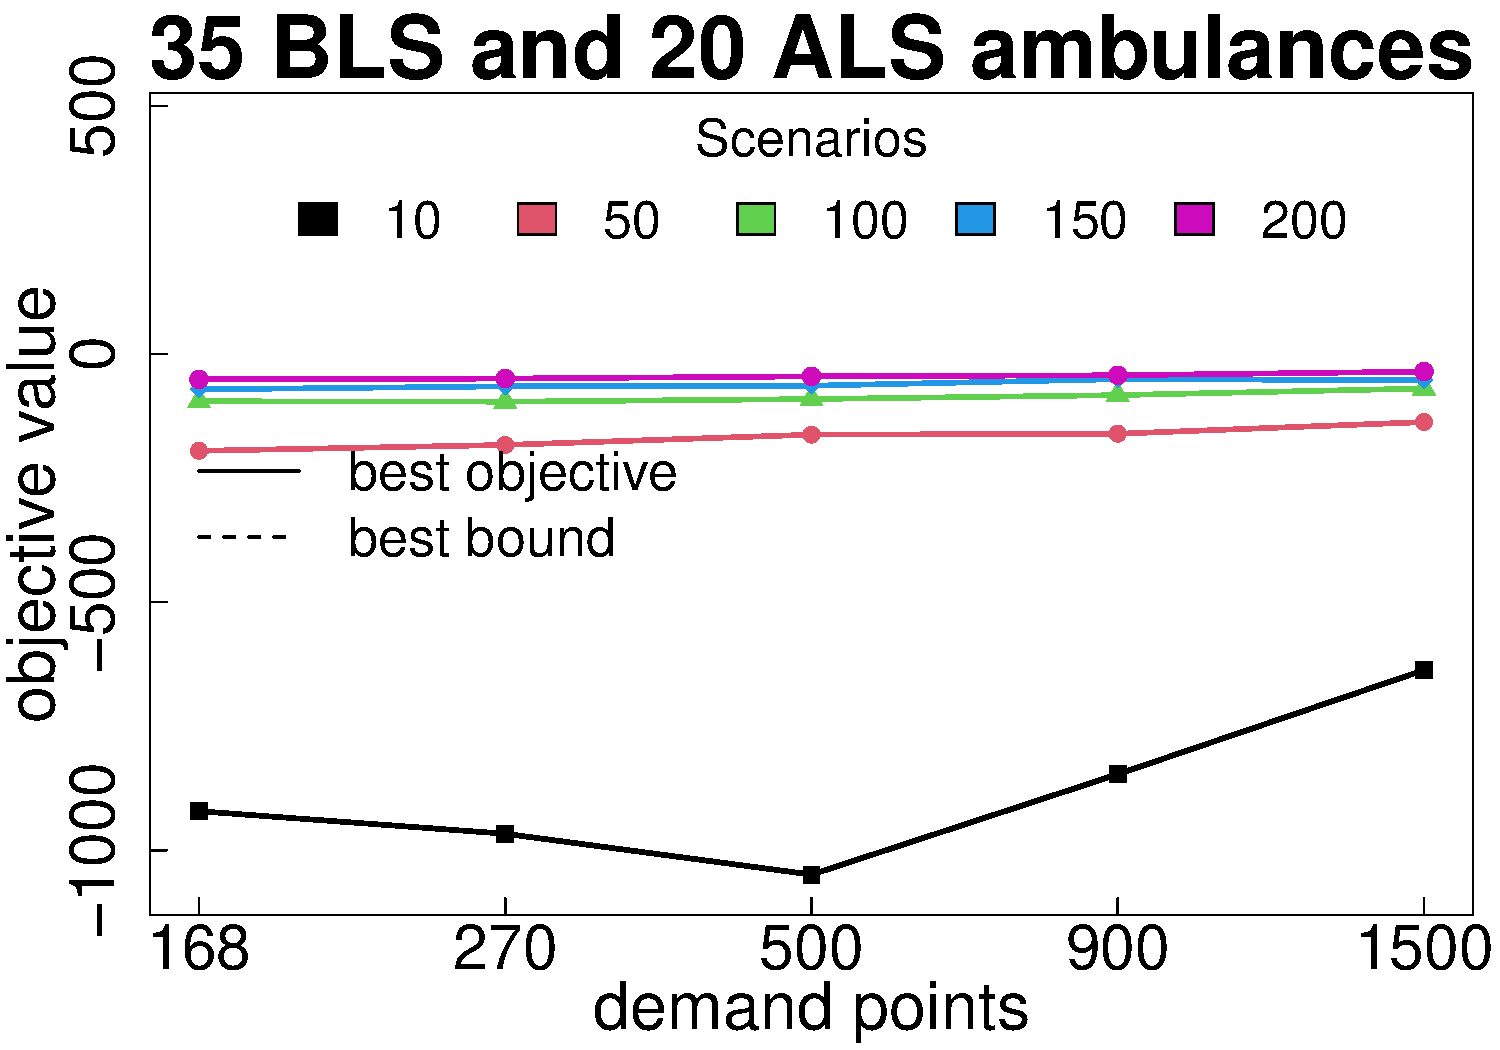
\includegraphics[width=0.42\textwidth]{Imagenes_Tesis/SABC/Obj_SABC_50.pdf}}{$|L|=50$}%
%\hspace{0.4cm}%
%\vspace{0.4cm}
%\stackunder[4pt]{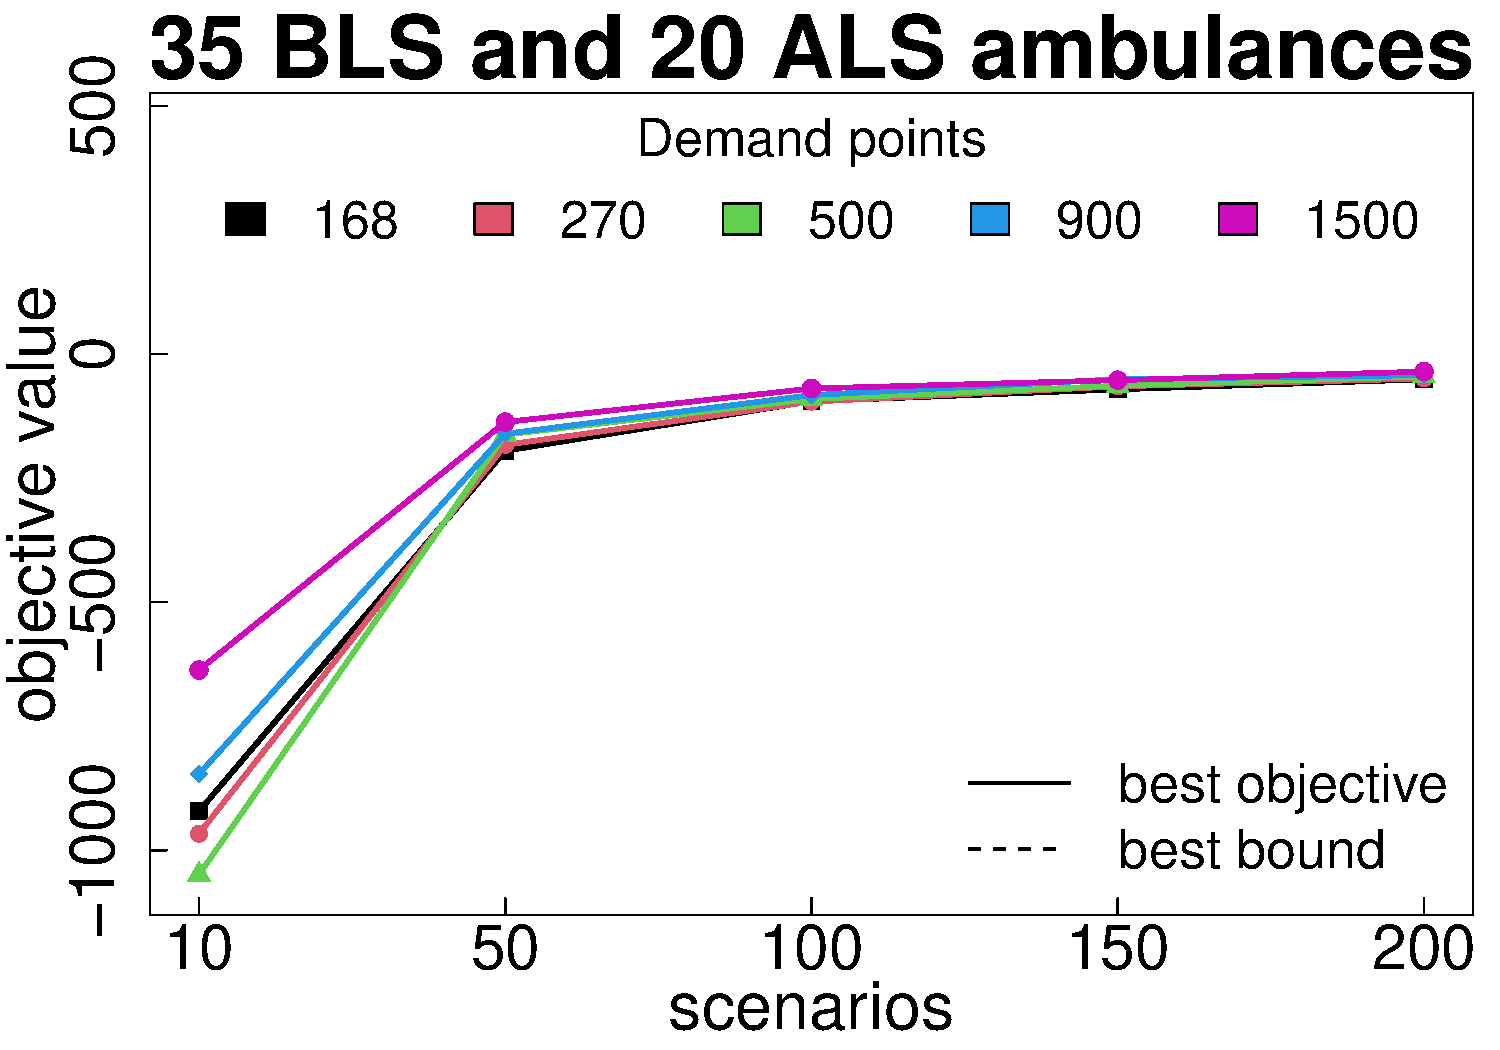
\includegraphics[width=0.42\textwidth]{Imagenes_Tesis/SABC/Obj_SABC_50_1.pdf}}{$|L|=50$}
%\stackunder[4pt]{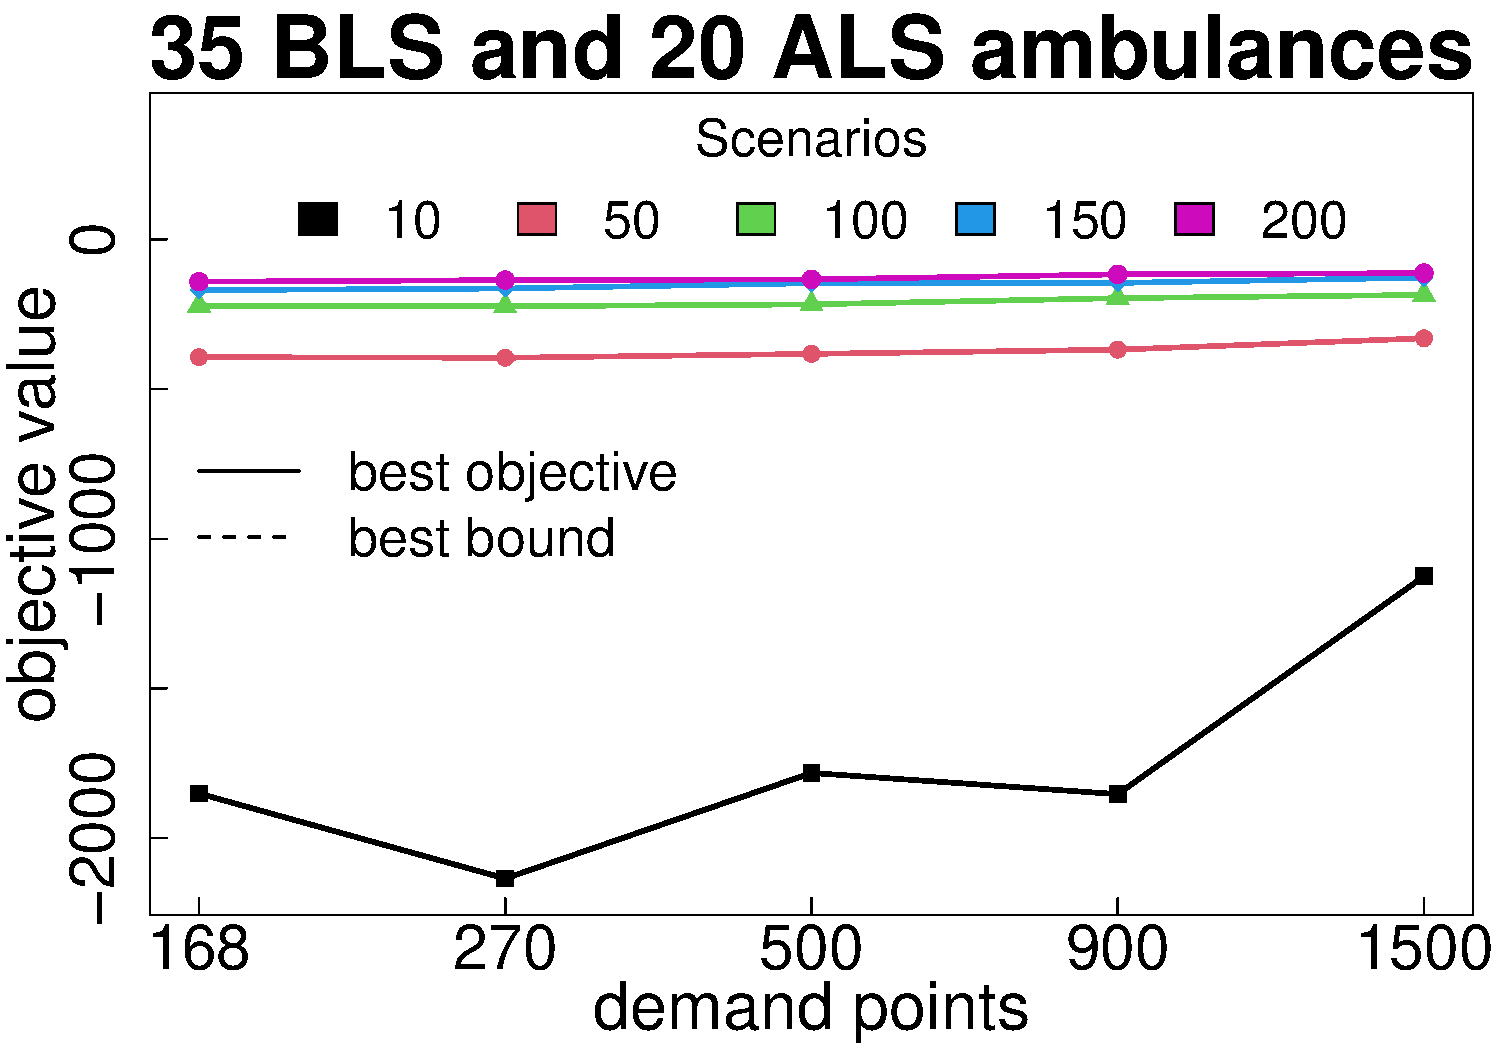
\includegraphics[width=0.42\textwidth]{Imagenes_Tesis/SABC/Obj_SABC_100.pdf}}{$|L|=100$}%
%\hspace{0.4cm}%
%\vspace{0.4cm}
%\stackunder[4pt]{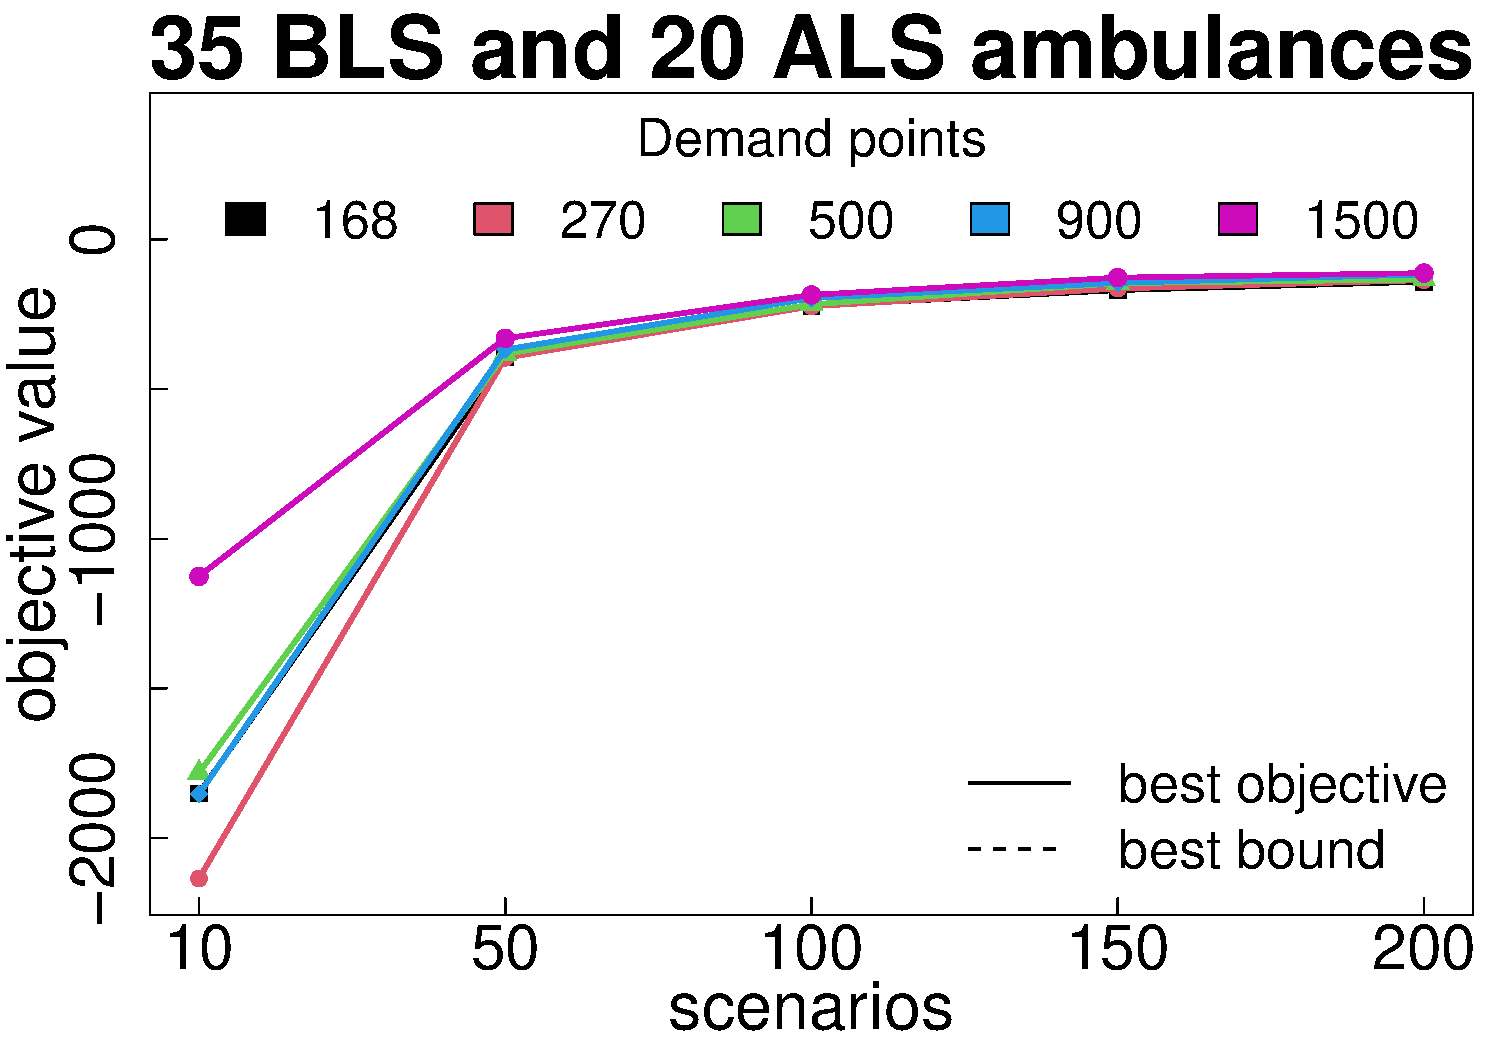
\includegraphics[width=0.42\textwidth]{Imagenes_Tesis/SABC/Obj_SABC_100_1.pdf}}{$|L|=100$}
%\caption{Objective SABC.}
%\label{Obj_SABC}
%\end{figure}


\section{Response time for the MEC, MEC(SABC) and SABC Matheuristic}
 The following experiment compares the running times of the equivalent MEC model with the MEC(SABC) method. Recall that MEC(SABC) attempts to exploit that the surrogate model SABC is very tractable and solved relatively quickly. To this end, Figure \ref{Time_MEC} shows plots of the running time in seconds of the instances with $|L|=16$, $|L|=50$ and $|L|=100$ potential location sites for the equivalent MEC, and Figure \ref{Time_M2M1} shows response times for the SBFM with the same potential sites. The x-axis of the plots corresponds to the number of scenarios, and we vary the number of emergency demand points. Recall that the MEC model with $|L|=\{50,100\}$ reaches the time limit even for ten scenarios and few demand points. 
 
 
\begin{figure}[H]
\centering
\footnotesize
\stackunder[4pt]{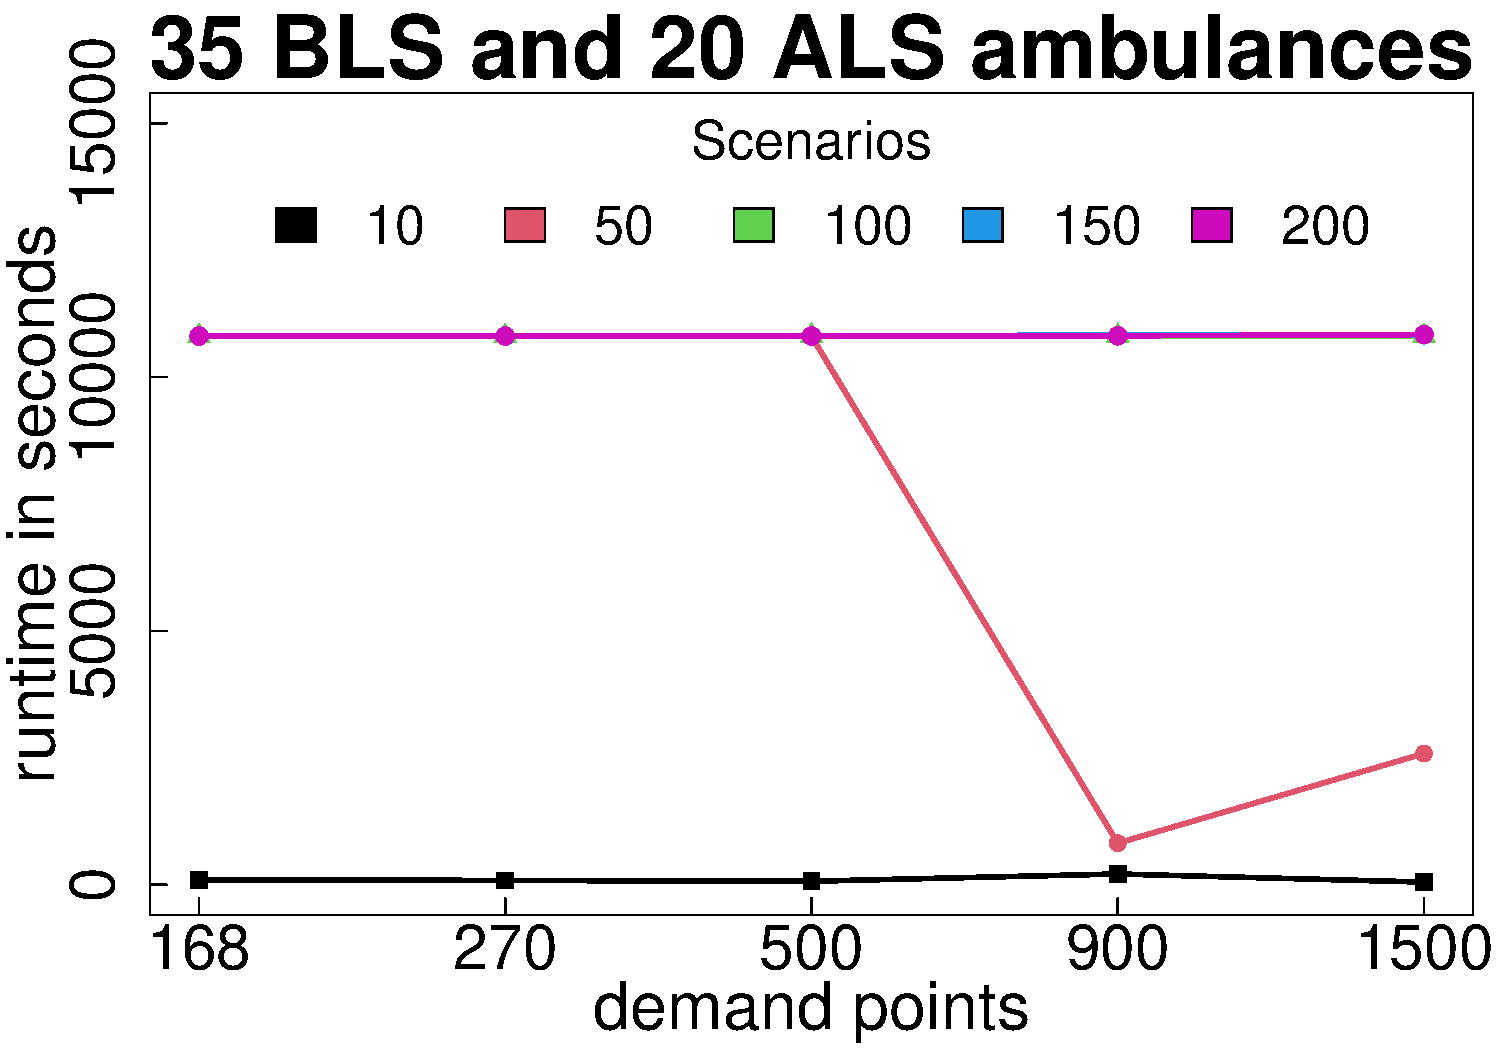
\includegraphics[width=0.42\textwidth]{Imagenes_Tesis/MEC/Time_MEC_16.pdf}}{$|L|=16$}%
\hspace{0.4cm}%
\vspace{0.4cm}
\stackunder[4pt]{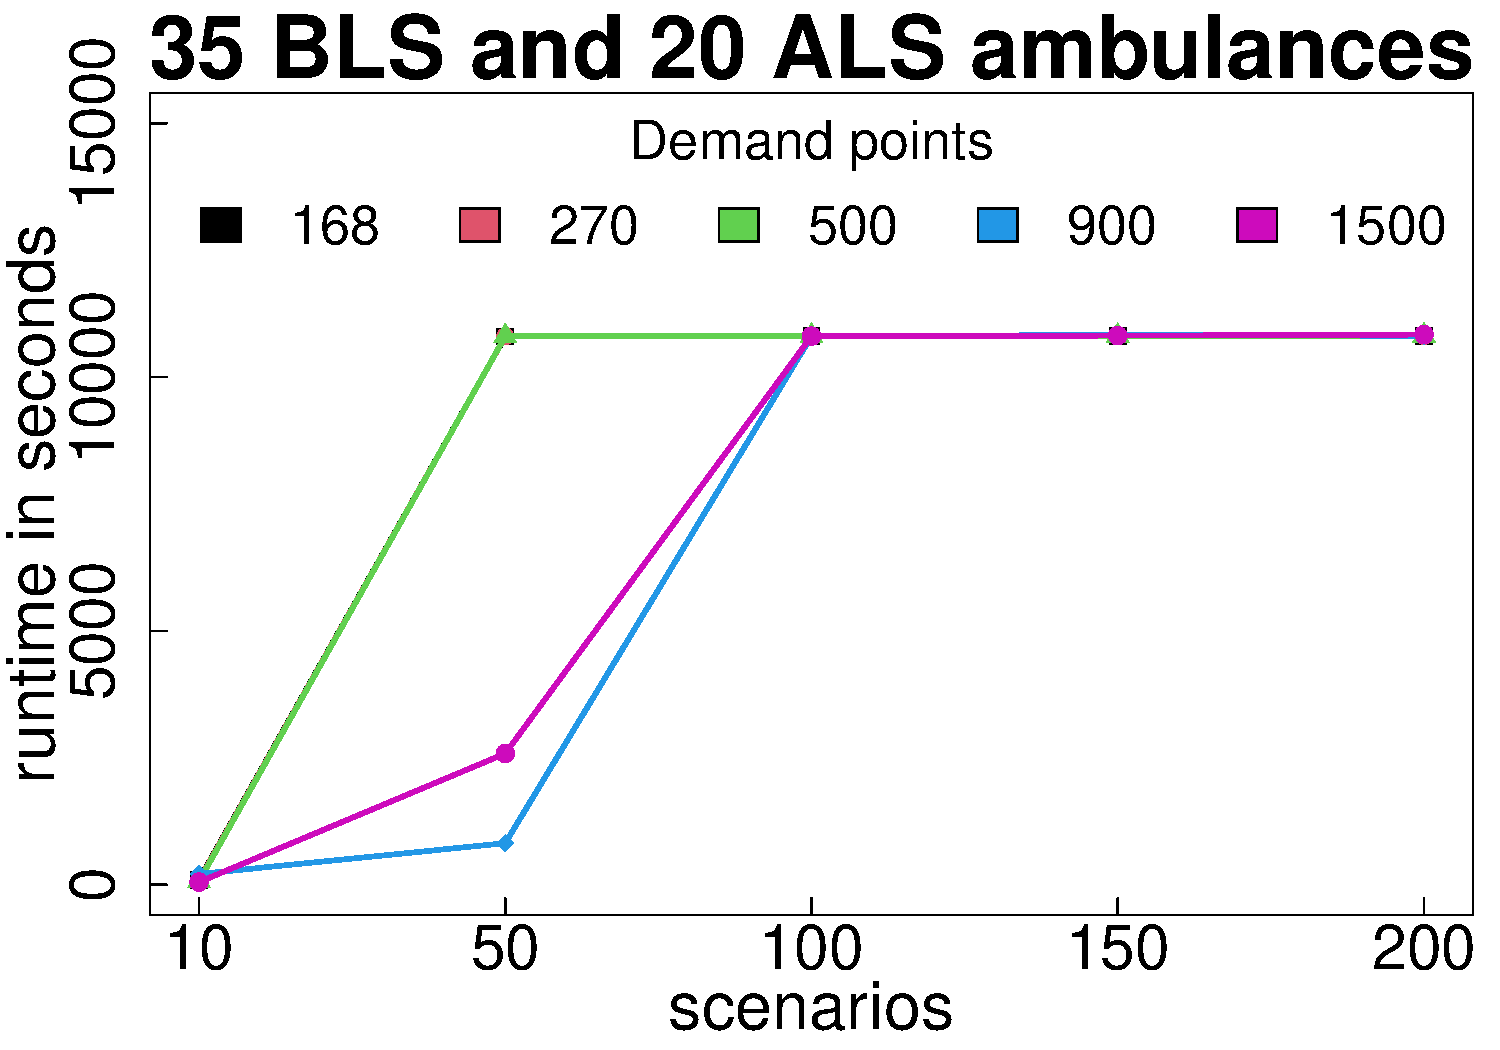
\includegraphics[width=0.42\textwidth]{Imagenes_Tesis/MEC/Time_MEC_16_1.pdf}}{$|L|=16$}
\stackunder[4pt]{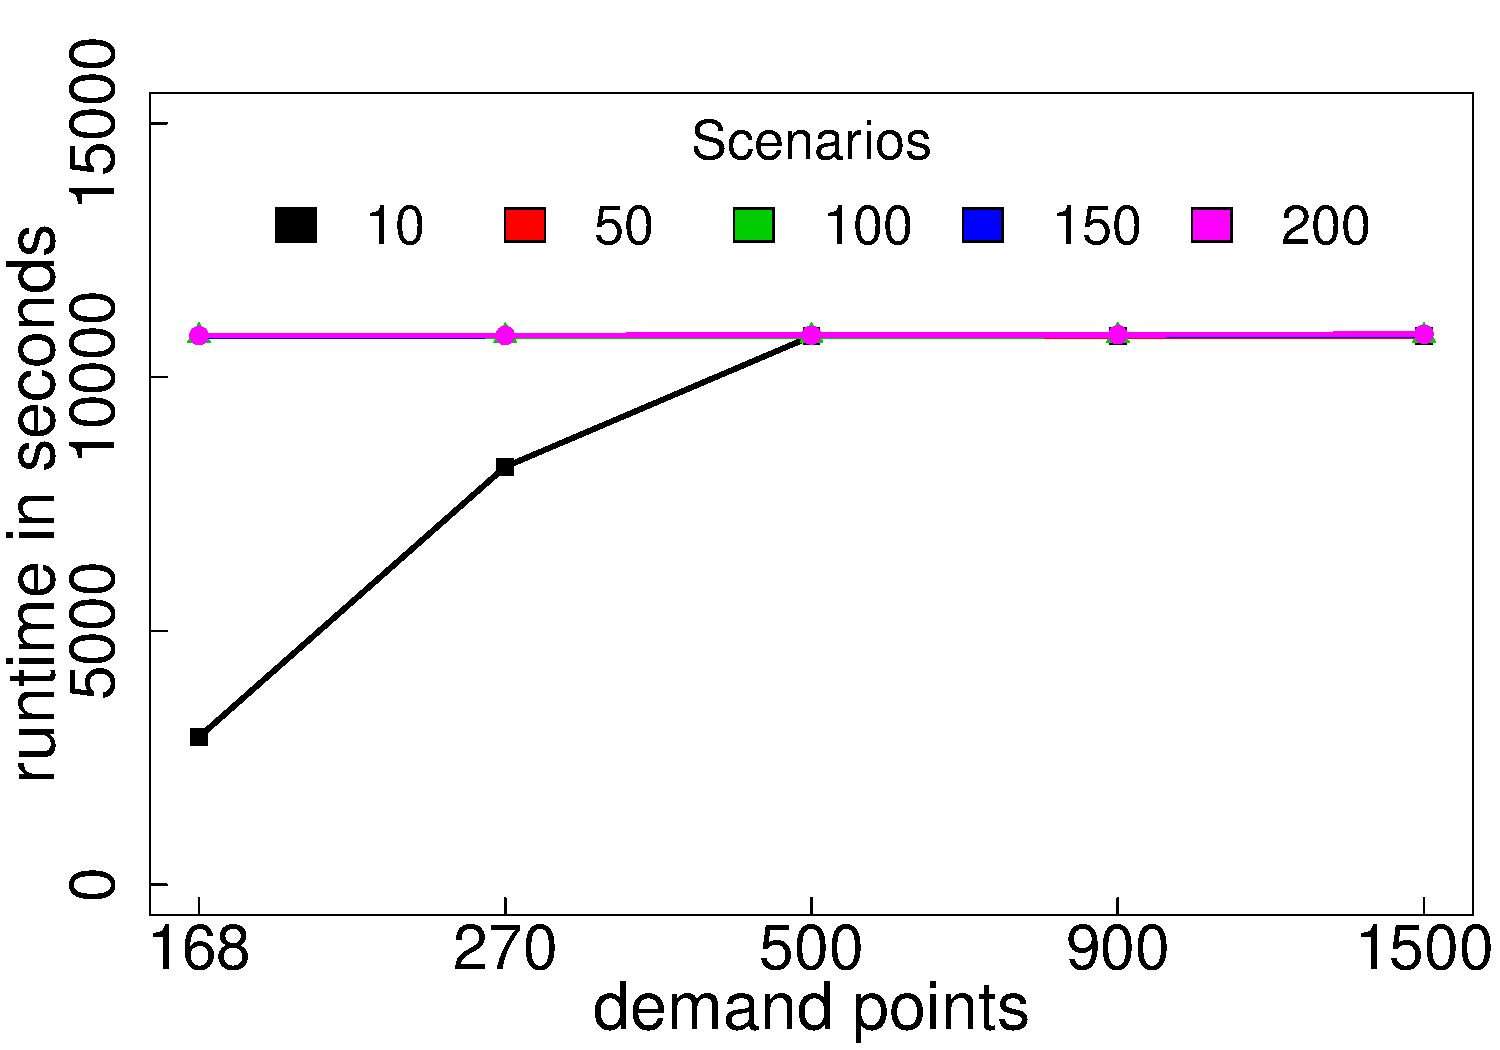
\includegraphics[width=0.42\textwidth]{Imagenes_Tesis/MEC/Time_MEC_50.pdf}}{$|L|=50$}%
\hspace{0.4cm}%
\vspace{0.4cm}
\stackunder[4pt]{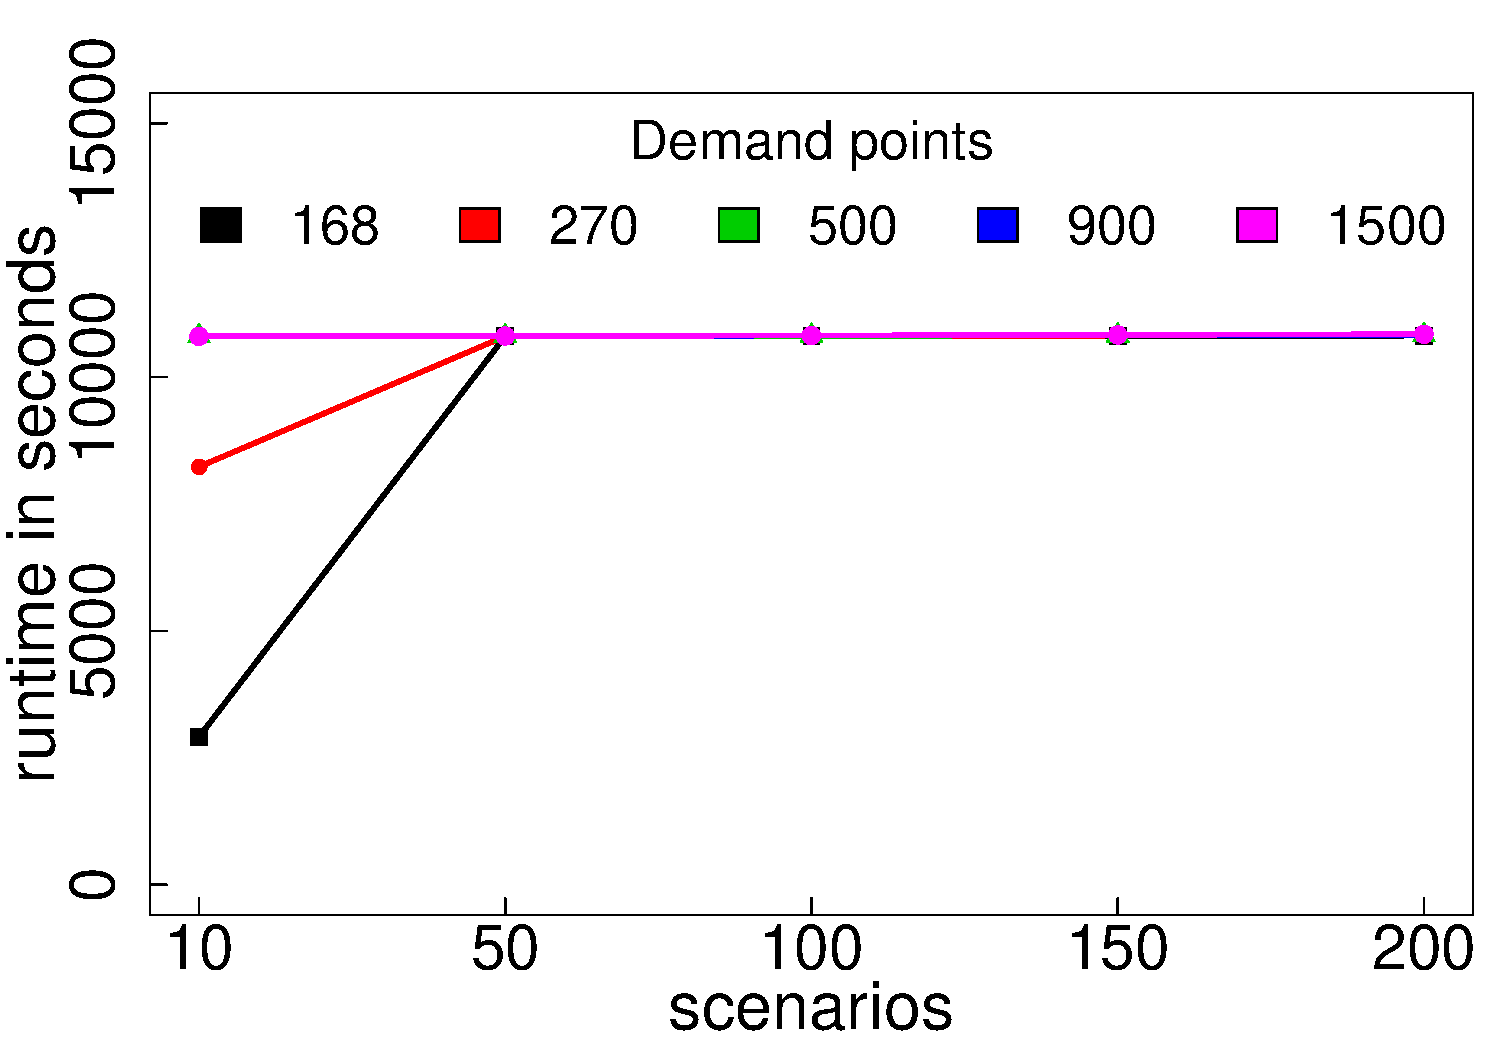
\includegraphics[width=0.42\textwidth]{Imagenes_Tesis/MEC/Time_MEC_50_1.pdf}}{$|L|=50$}
\stackunder[4pt]{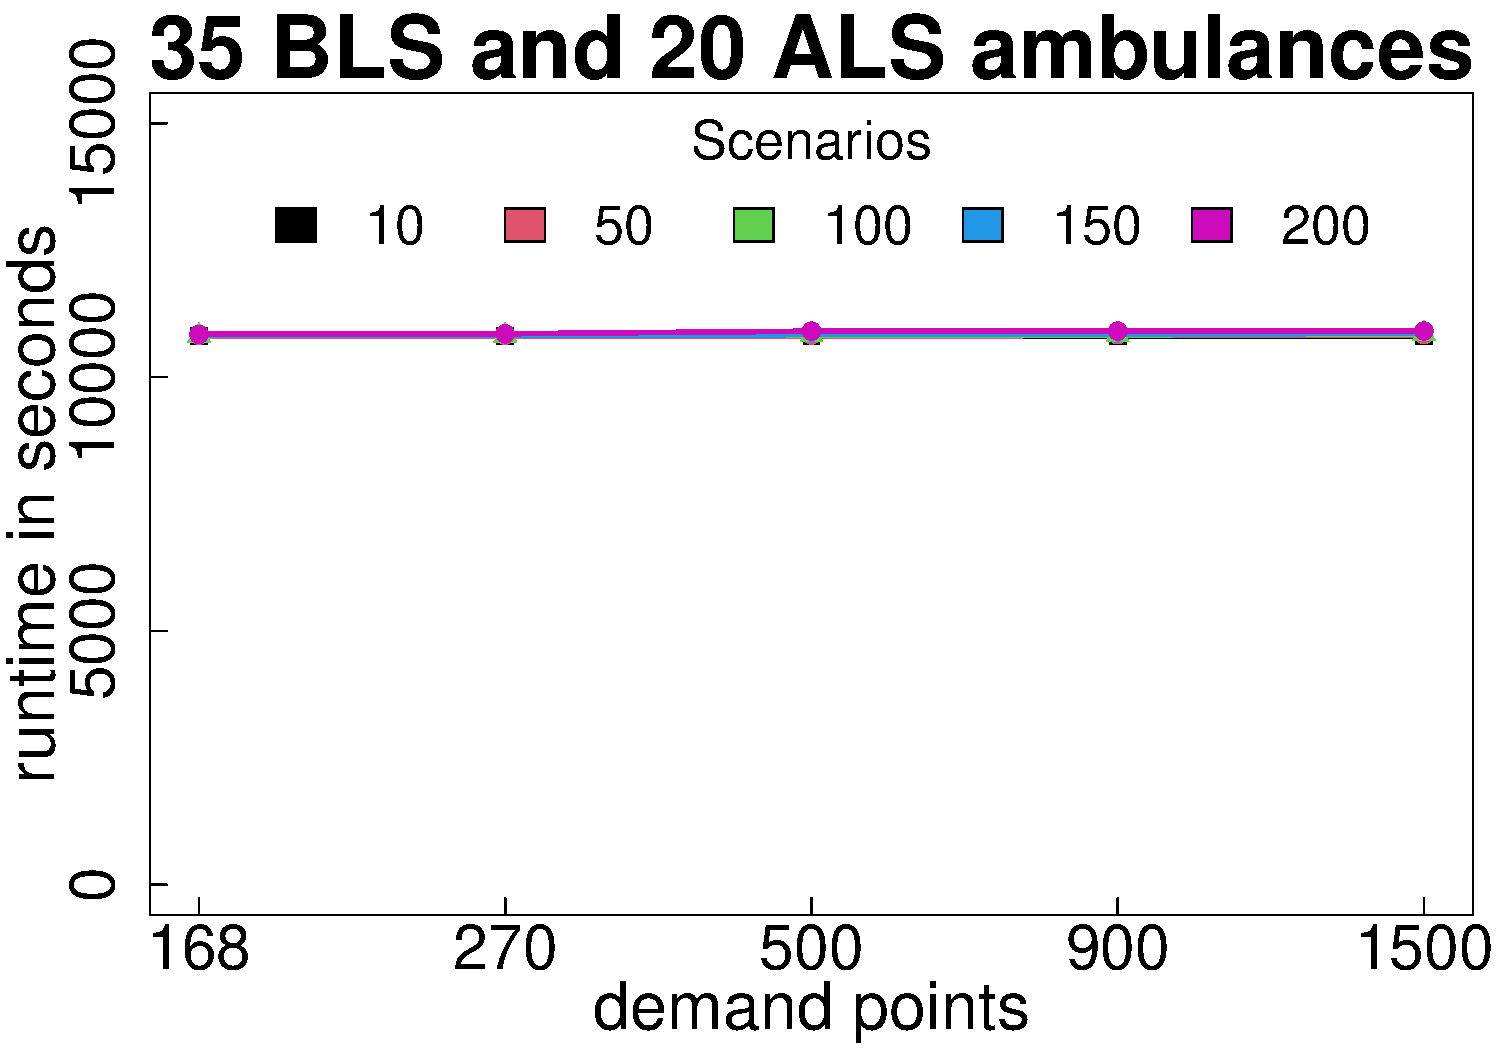
\includegraphics[width=0.42\textwidth]{Imagenes_Tesis/MEC/Time_MEC_100.pdf}}{$|L|=100$}%
\hspace{0.4cm}%
\vspace{0.4cm}
\stackunder[4pt]{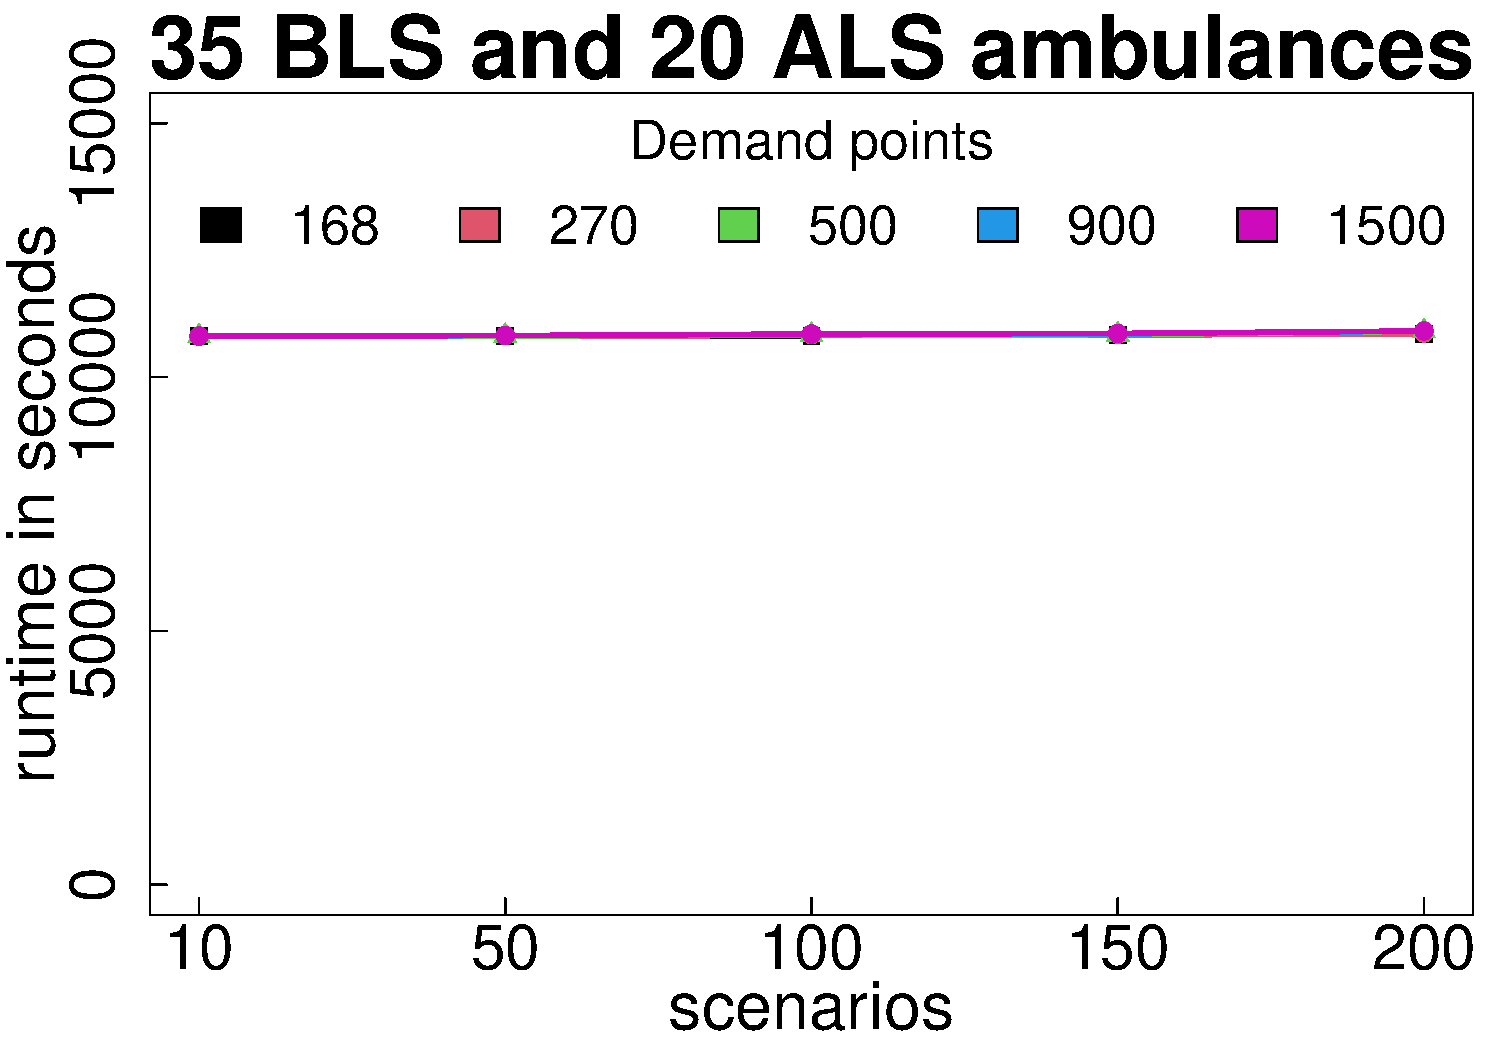
\includegraphics[width=0.42\textwidth]{Imagenes_Tesis/MEC/Time_MEC_100_1.pdf}}{$|L|=100$}
\caption{Time MEC.}
\label{Time_MEC}
\end{figure} 


\begin{figure}[H]
\centering
\footnotesize
\stackunder[4pt]{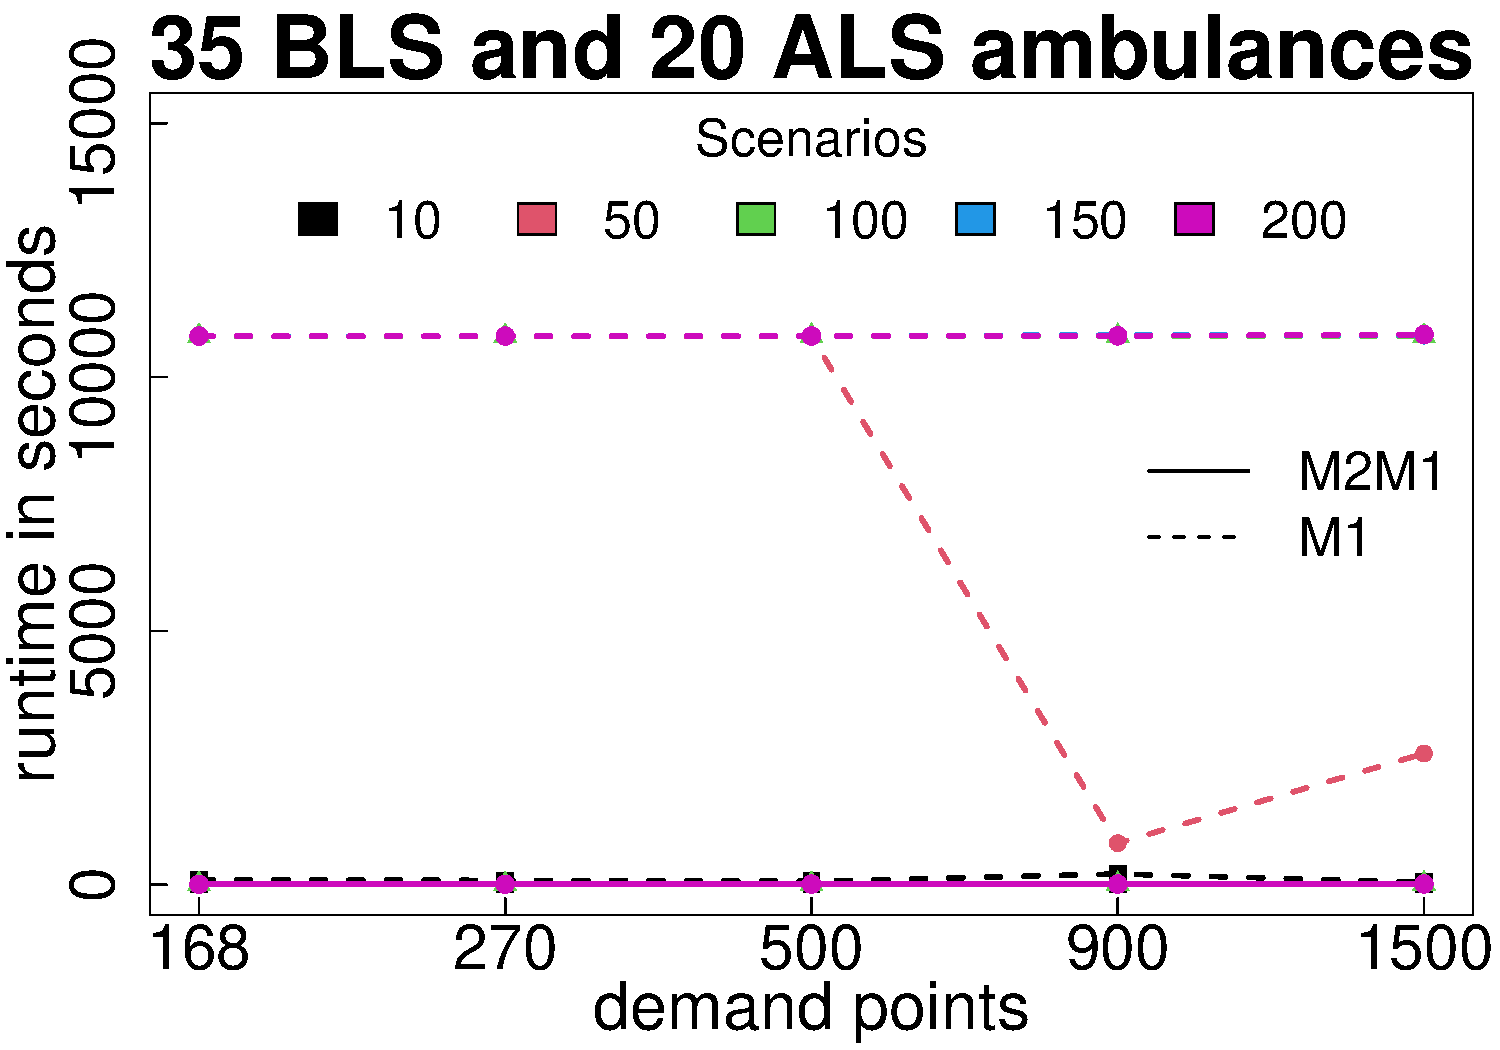
\includegraphics[width=0.42\textwidth]{Imagenes_Tesis/M2M1/Time_M2M1_16.pdf}}{$|L|=16$}%
\hspace{0.4cm}%
\vspace{0.4cm}
\stackunder[4pt]{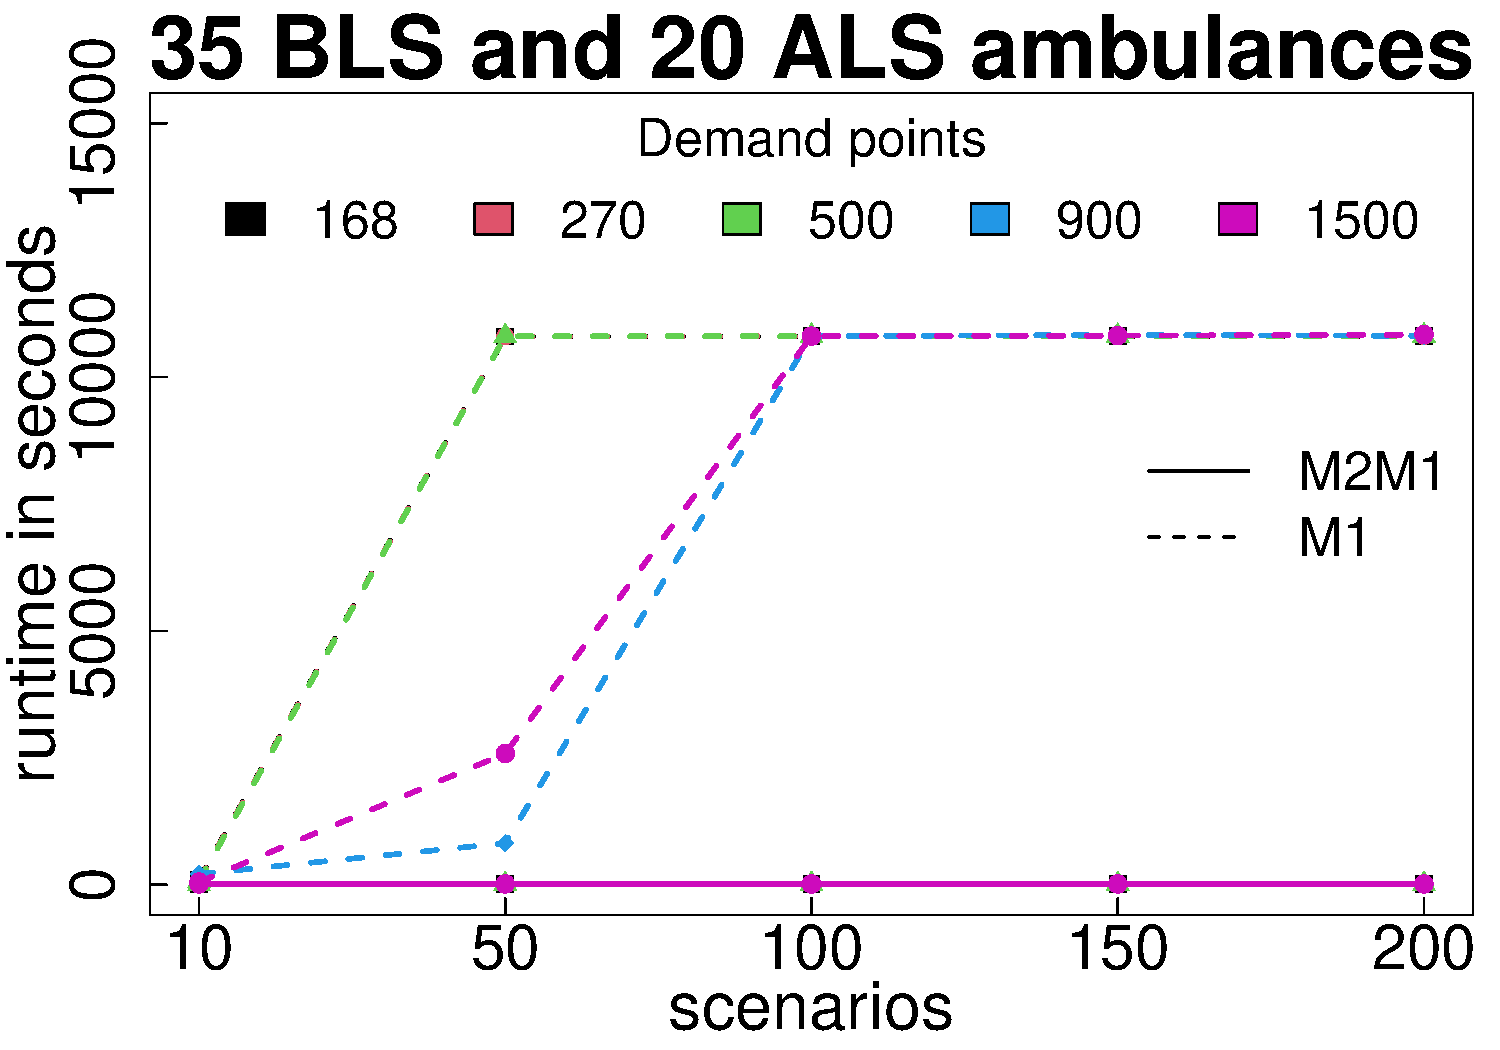
\includegraphics[width=0.42\textwidth]{Imagenes_Tesis/M2M1/Time_M2M1_16_1.pdf}}{$|L|=16$}
\stackunder[4pt]{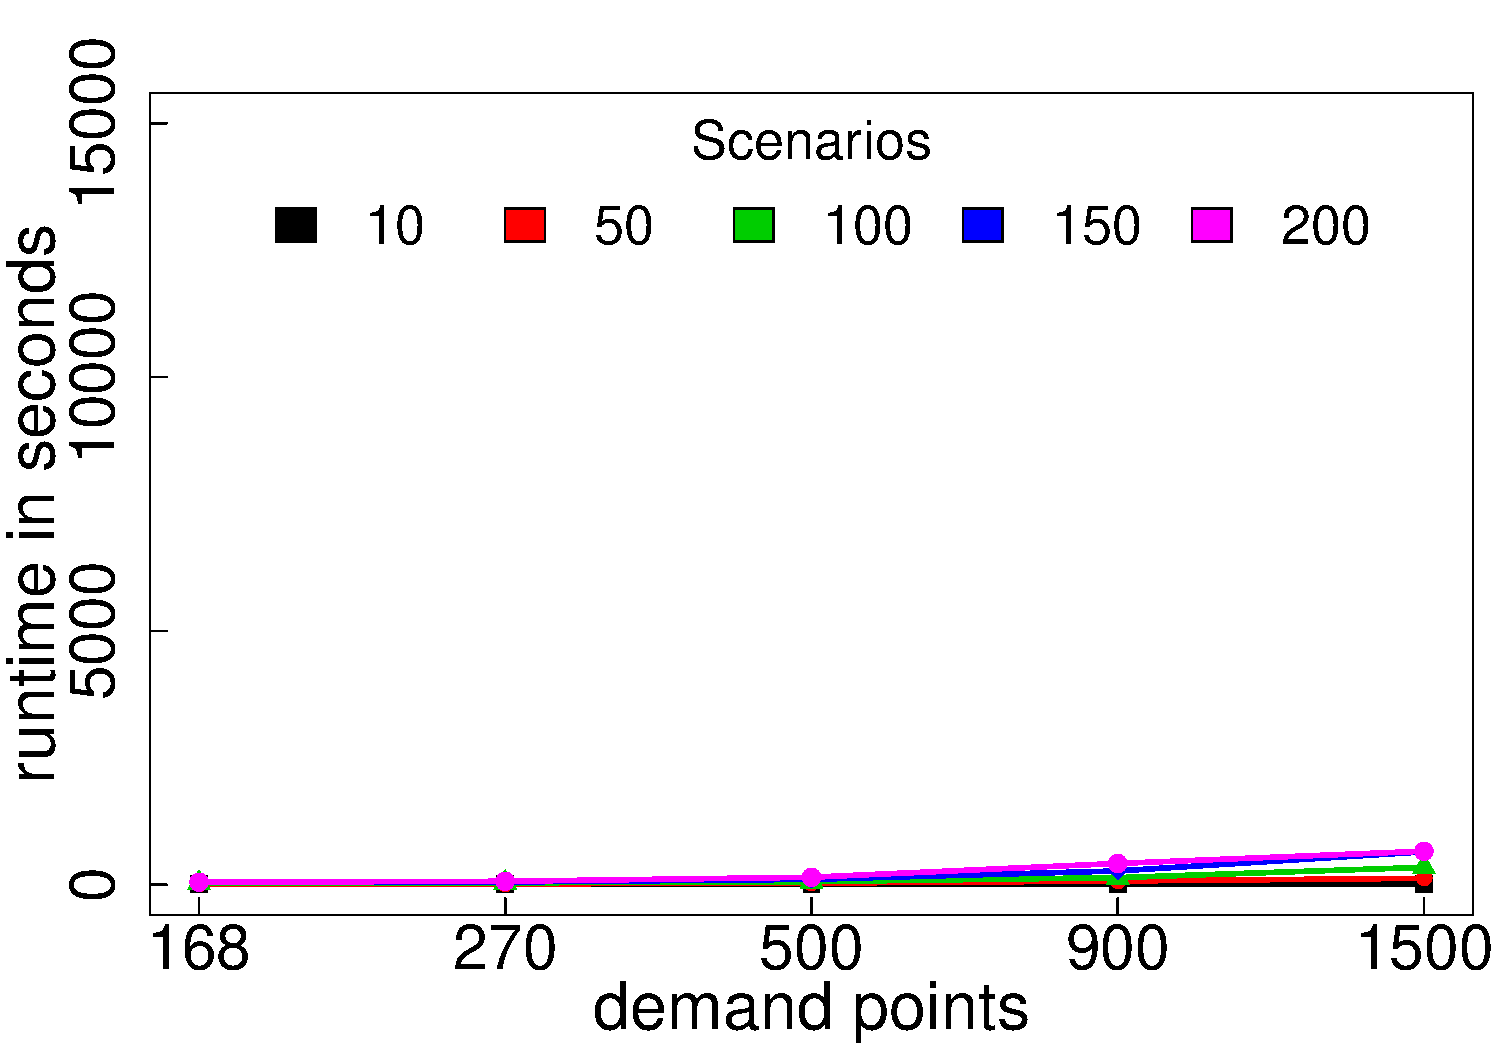
\includegraphics[width=0.42\textwidth]{Imagenes_Tesis/M2M1/Time_M2M1_50.pdf}}{$|L|=50$}%
\hspace{0.4cm}%
\vspace{0.4cm}
\stackunder[4pt]{\includegraphics[width=0.42\textwidth]{Imagenes_Tesis/M2M1/Time_M2M1_50_1.pdf}}{$|L|=50$}
\stackunder[4pt]{\includegraphics[width=0.42\textwidth]{Imagenes_Tesis/M2M1/Time_M2M1_100.pdf}}{$|L|=100$}%
\hspace{0.4cm}%
\vspace{0.4cm}
\stackunder[4pt]{\includegraphics[width=0.42\textwidth]{Imagenes_Tesis/M2M1/Time_M2M1_100_1.pdf}}{$|L|=100$}
\caption{Time M2M1.}
\label{Time_M2M1}
\end{figure}
 
%\begin{figure}[!tb]
%  \begin{center}
%    \subfigure[MEC with $|L|=16$.]{
%    \includegraphics[width=0.48\textwidth]{M1Time16.png}}
%    %\subfigure[ SABC model with 100 potential sites]{
%        %\includegraphics[width=0.45\textwidth]{figures/M2Time100.png}
%     %}
%        \subfigure[MEC(SABC) with $|L|=100$.]{
%        \includegraphics[width=0.45\textwidth]{M1M2Time.png}
%         }
%    \caption{Computational time for the a) MEC and b) MEC(SABC) model concerning the number of scenarios varying the number of emergency demand points.}
%    \label{M1M2Time}
%  \end{center}
%\end{figure}

Figure \ref{Time_MEC} shows that the main disadvantage of the MEC model is its computational time, which increases significantly with the number of demand points, potential sites, and scenarios, even for small instances with 16 potential location sites for ambulances. The SABC model is extremely fast, even for large instances, and yields an initial solution to the assignment of ambulance location in a short time to allow the MEC(SABC) model, Figure \ref{Time_M2M1}, to be solved faster than the MEC model and obtain high-quality solutions. The MEC(SABC) location-allocation strategy inherits not only its fast computational time from the SABC, but also yields coverage per emergency situation, which is the main objective for the EVCP problem. The MEC(SABC) model is an approximated mathod, but it gives solutions that are as good as the MEC and even better when the MEC instances do not reach optimality and its gaps are large. The SBFM solves most instances in less than a minute.  

An interesting advantage of the SBFM is that only one iteration is needed. In fact, once the location of the ambulances has been retrieved from the SABC model and fed back to the MEC model, we could perturb the ambulances either randomly or with a local search, the allocation of the ambulances, and iterate again. Nevertheless, we could not systematically generate a neighborhood around a location solution that yields better solutions with the MEC(SABC) approach. This implies that local maximums are often reached with this first feedback and that complex or more diverse neighborhoods should be built to allow escaping from these solutions. It would probably be interesting to enable local search movements that do not yield immediate benefits.  

Comparing SABC Matheuristic runtime with MEC and MEC(SABC) we show Figure \ref{Time_Comp}. MEC still has a very large computational time compared to the other two methodologies. As we can see, MEC(SABC) methodology computaional time is always less or equal to SABC MAtheuristic computational time. Even SABC Matheuristic is a local search procedure, the evaluation in MEC(SABC) for each neighbor increases the computational time when instances are large. Still, it is not a time that should alarm us, which indicates that it is a good procedure.


\begin{figure}[H]
\centering
\footnotesize
\stackunder[4pt]{\includegraphics[width=0.42\textwidth]{Imagenes_Tesis/Comp/Time_Comp_16.pdf}}{$|L|=16$}%
\hspace{0.4cm}%
\vspace{0.4cm}
\stackunder[4pt]{\includegraphics[width=0.42\textwidth]{Imagenes_Tesis/Comp/Time_Comp_16_1.pdf}}{$|L|=16$}
\stackunder[4pt]{\includegraphics[width=0.42\textwidth]{Imagenes_Tesis/Comp/Time_Comp_50.pdf}}{$|L|=50$}%
\hspace{0.4cm}%
\vspace{0.4cm}
\stackunder[4pt]{\includegraphics[width=0.42\textwidth]{Imagenes_Tesis/Comp/Time_Comp_50_1.pdf}}{$|L|=50$}
\stackunder[4pt]{\includegraphics[width=0.42\textwidth]{Imagenes_Tesis/Comp/Time_Comp_100.pdf}}{$|L|=100$}%
\hspace{0.4cm}%
\vspace{0.4cm}
\stackunder[4pt]{\includegraphics[width=0.42\textwidth]{Imagenes_Tesis/Comp/Time_Comp_100_1.pdf}}{$|L|=100$}
\caption{Time Comp.}
\label{Time_Comp}
\end{figure}


%\begin{figure}[H]
%\centering
%\footnotesize
%\stackunder[4pt]{\includegraphics[width=0.42\textwidth]{Imagenes_Tesis/SABC/Time_SABC_16.pdf}}{}%
%\hspace{0.4cm}%
%\vspace{0.4cm}
%\stackunder[4pt]{\includegraphics[width=0.42\textwidth]{Imagenes_Tesis/SABC/Time_SABC_16_1.pdf}}{}
%\stackunder[4pt]{\includegraphics[width=0.42\textwidth]{Imagenes_Tesis/SABC/Time_SABC_50.pdf}}{}%
%\hspace{0.4cm}%
%\vspace{0.4cm}
%\stackunder[4pt]{\includegraphics[width=0.42\textwidth]{Imagenes_Tesis/SABC/Time_SABC_50_1.pdf}}{}
%\stackunder[4pt]{\includegraphics[width=0.42\textwidth]{Imagenes_Tesis/SABC/Time_SABC_100.pdf}}{}%
%\hspace{0.4cm}%
%\vspace{0.4cm}
%\stackunder[4pt]{\includegraphics[width=0.42\textwidth]{Imagenes_Tesis/SABC/Time_SABC_100_1.pdf}}{}
%\caption{Time SABC.}
%\label{Time_SABC}
%\end{figure}
%
%
%\begin{figure}[H]
%\centering
%\footnotesize
%\stackunder[4pt]{\includegraphics[width=0.42\textwidth]{Imagenes_Tesis/Math/Time_Math_16.pdf}}{}%
%\hspace{0.4cm}%
%\vspace{0.4cm}
%\stackunder[4pt]{\includegraphics[width=0.42\textwidth]{Imagenes_Tesis/Math/Time_Math_16_1.pdf}}{}
%\stackunder[4pt]{\includegraphics[width=0.42\textwidth]{Imagenes_Tesis/Math/Time_Math_50.pdf}}{}%
%\hspace{0.4cm}%
%\vspace{0.4cm}
%\stackunder[4pt]{\includegraphics[width=0.42\textwidth]{Imagenes_Tesis/Math/Time_Math_50_1.pdf}}{}
%\stackunder[4pt]{\includegraphics[width=0.42\textwidth]{Imagenes_Tesis/Math/Time_Math_100.pdf}}{}%
%\hspace{0.4cm}%
%\vspace{0.4cm}
%\stackunder[4pt]{\includegraphics[width=0.42\textwidth]{Imagenes_Tesis/Math/Time_Math_100_1.pdf}}{}
%\caption{Time Math.}
%\label{Time_Math}
%\end{figure}
%



\section{Coverage for the MEC, MEC(SABC) and SABC Matheuristic}

 The objective values and running times are crucial for evaluating the models' performance. However, the most critical objective of the EVCP problem is to cover the largest number of demand points within a fixed response time. Thus, a central question arises: Is the emergency coverage quality of the MEC(SABC) as good as the one yielded by the MEC model?  
 
The percentage of emergency coverage for all instances is presented with the equivalent MEC model and the SBFM in Figures \ref{Cov_MEC} and \ref{Cov_M2M1} respectively.. Two columns with three plots each, varying the number of scenarios and the location sites. Each plot shows the type of ambulance percentage coverage obtained¿: T is for Total coverage (all required ambulances on time), TL is for Total-late coverage (all required ambulances, but at least one arrives late), P is for Partial coverage (at least one required ambulance is not dispatched, but the dispatched ones all arrive in time), PL is for Partial-late coverage (at least one required ambulance is not dispatched, at least one of the dispatched arrives late), and N for Null (no ambulances assigned to the demand point). The upper plots are for  $|L|=\{16\}$ potential sites, the middle ones for $|L|=50$, and the lower ones for $|L|=100$.

\begin{figure}[H]
\centering
\footnotesize
\stackunder[4pt]{\includegraphics[width=0.42\textwidth]{Imagenes_Tesis/MEC/Cov_MEC_16.pdf}}{$|L|=16$}%
\hspace{0.4cm}%
\vspace{0.4cm}
\stackunder[4pt]{\includegraphics[width=0.42\textwidth]{Imagenes_Tesis/MEC/Cov_MEC_16_1.pdf}}{$|L|=16$}
\stackunder[4pt]{\includegraphics[width=0.42\textwidth]{Imagenes_Tesis/MEC/Cov_MEC_50.pdf}}{$|L|=50$}%
\hspace{0.4cm}%
\vspace{0.4cm}
\stackunder[4pt]{\includegraphics[width=0.42\textwidth]{Imagenes_Tesis/MEC/Cov_MEC_50_1.pdf}}{$|L|=50$}
\stackunder[4pt]{\includegraphics[width=0.42\textwidth]{Imagenes_Tesis/MEC/Cov_MEC_100.pdf}}{$|L|=100$}%
\hspace{0.4cm}%
\vspace{0.4cm}
\stackunder[4pt]{\includegraphics[width=0.42\textwidth]{Imagenes_Tesis/MEC/Cov_MEC_100_1.pdf}}{$|L|=100$}
\caption{Coverage MEC.}
\label{Cov_MEC}
\end{figure}

   

%\begin{figure}[htb]
%    \centering
%    \includegraphics[width=0.8\linewidth]{CoverageTodos.png}
%    \caption{Coverage percentage per type obtained by the a) MEC model and the b) SBFM for potential sites $|L|=\{16,50,100\}$.}
%    \label{fig:Coverage}
%\end{figure}

Figure \ref{Cov_MEC}, shows that the MEC model tends to leave very few demand points with null coverage, which is the primary concern of the emergency services in our case study. As the number of potential sites $|L|$ increases, the coverage tends to be partial-late for the MEC model. This behavior is probably related to the large gaps obtained by the MEC model for large instances, but the number of null coverage is still remarkably low.  
Figure \ref{Cov_M2M1} shows that the SBFM is robust in terms of the number of scenarios. That is, the demand point coverage is independent of the scenario number. In this way, 100 scenarios are sufficient to handle a high-quality coverage solution. Moreover, the MEC(SABC) model inherits the characteristic of having very few null demand point coverage from the MEC model. Interestingly, partial coverage tends to be larger than partial late coverage, which is mainly desired in real life because it can be translated into first-aid medical care on time, increasing the probability of saving lives. 

\begin{figure}[H]
\centering
\footnotesize
\stackunder[4pt]{\includegraphics[width=0.42\textwidth]{Imagenes_Tesis/M2M1/Cov_M2M1_16.pdf}}{$|L|=16$}%
\hspace{0.4cm}%
\vspace{0.4cm}
\stackunder[4pt]{\includegraphics[width=0.42\textwidth]{Imagenes_Tesis/M2M1/Cov_M2M1_16_1.pdf}}{$|L|=16$}
\stackunder[4pt]{\includegraphics[width=0.42\textwidth]{Imagenes_Tesis/M2M1/Cov_M2M1_50.pdf}}{$|L|=50$}%
\hspace{0.4cm}%
\vspace{0.4cm}
\stackunder[4pt]{\includegraphics[width=0.42\textwidth]{Imagenes_Tesis/M2M1/Cov_M2M1_50_1.pdf}}{$|L|=50$}
\stackunder[4pt]{\includegraphics[width=0.42\textwidth]{Imagenes_Tesis/M2M1/Cov_M2M1_100.pdf}}{$|L|=100$}%
\hspace{0.4cm}%
\vspace{0.4cm}
\stackunder[4pt]{\includegraphics[width=0.42\textwidth]{Imagenes_Tesis/M2M1/Cov_M2M1_100_1.pdf}}{$|L|=100$}
\caption{Coverage M2M1.}
\label{Cov_M2M1}
\end{figure}

For the SABC Matheuristic the coverage results are in Figure \ref{Cov_Math}. As we saw in Figure \ref{Cov_M2M1}, SABC Matheuristic tends to have a large partial coverage. The results are for the best neighbor found throughout the matheuristic, which has not a significant difference to the MEC(SABC) results.

\begin{figure}[H]
\centering
\footnotesize
\stackunder[4pt]{\includegraphics[width=0.42\textwidth]{Imagenes_Tesis/Math/Cov_Math_16.pdf}}{$|L|=16$}%
\hspace{0.4cm}%
\vspace{0.4cm}
\stackunder[4pt]{\includegraphics[width=0.42\textwidth]{Imagenes_Tesis/Math/Cov_Math_16_1.pdf}}{$|L|=16$}
\stackunder[4pt]{\includegraphics[width=0.42\textwidth]{Imagenes_Tesis/Math/Cov_Math_50.pdf}}{$|L|=50$}%
\hspace{0.4cm}%
\vspace{0.4cm}
\stackunder[4pt]{\includegraphics[width=0.42\textwidth]{Imagenes_Tesis/Math/Cov_Math_50_1.pdf}}{$|L|=50$}
\stackunder[4pt]{\includegraphics[width=0.42\textwidth]{Imagenes_Tesis/Math/Cov_Math_100.pdf}}{$|L|=100$}%
\hspace{0.4cm}%
\vspace{0.4cm}
\stackunder[4pt]{\includegraphics[width=0.42\textwidth]{Imagenes_Tesis/Math/Cov_Math_100_1.pdf}}{$|L|=100$}
\caption{Coverage Math.}
\label{Cov_Math}
\end{figure}


%\subsection{Number of ambulances available in the system}\label{num amb}

 All the previous experiments were executed with the number of ambulances equal to $(\eta_1,\eta_2)=   (35,20) $. A central feature of the EVCP problem is that an ALS ambulance can be sent instead of the BLS one, which gives a more flexible setting but may induce difficulty when solving the models. 
 Thus, what is the effect of the number of available ambulances in the EVCP problem on the objective function value and the running time?

For a preliminary evaluation we launched experiments changing the number of ambulances for the MEC problem considering $|L|=16$ potential sites for all sizes of demand points and scenarios. Figure \ref{Obj_Prelim} presents objective values. As we expected, the number of ambulances increases the gap between best objective and best bound found in some cases, mostly when the number of scenarios increases for  $(\eta_1,\eta_2)$=(10,6) and (20,11). Although, as the number of ambulances increases, the gap decreases, and we decided to reduce our instances set considering just $(\eta_1,\eta_2)$=(35,20) to obtain more realistic results according to the number of ambulances in our case of the EMS system in Nuevo León. Besides, in Figure \ref{Time_Prelim} we can see there is a none significant difference for the runtime varying the number of ambulances so considering a few number of them does not help the model to use a low computational time.

\begin{figure}[H]
\centering
\footnotesize
\stackunder[4pt]{\includegraphics[width=0.48\textwidth]{Imagenes_Tesis/Preliminar/Objval_10_6.pdf}}{}%
\hspace{0.4cm}%
\vspace{0.4cm}
\stackunder[4pt]{\includegraphics[width=0.48\textwidth]{Imagenes_Tesis/Preliminar/Objval_20_11.pdf}}{}
\stackunder[4pt]{\includegraphics[width=0.48\textwidth]{Imagenes_Tesis/Preliminar/Objval_35_20.pdf}}{}%
\hspace{0.4cm}%
\vspace{0.4cm}
\caption{Objective preliminar.}
\label{Obj_Prelim}
\end{figure}
  
  
\begin{figure}[H]
\centering
\footnotesize
\stackunder[4pt]{\includegraphics[width=0.48\textwidth]{Imagenes_Tesis/Preliminar/Timeval_10_6.pdf}}{}%
\hspace{0.4cm}%
\vspace{0.4cm}
\stackunder[4pt]{\includegraphics[width=0.48\textwidth]{Imagenes_Tesis/Preliminar/Timeval_20_11.pdf}}{}
\stackunder[4pt]{\includegraphics[width=0.48\textwidth]{Imagenes_Tesis/Preliminar/Timeval_35_20.pdf}}{}%
\hspace{0.4cm}%
\vspace{0.4cm}
\caption{Time preliminar.}
\label{Time_Prelim}
\end{figure}

 We execute all the instances with emergency demand points fixed to 900, 100 scenarios, and 50 ambulance location sites. For this experiment, we vary the number of ambulances. Figure \ref{fig:amb} shows two columns of two plots each. The objective value (upper plots) and the running time (lower plots) are on the y-axis, while the x-axis varies the number of ambulances: $(\eta_1,\eta_2)$=(10,6), (20,11), and  $(\eta_1,\eta_2)$=m,(35,20). The left plots correspond to the MEC stochastic model, while the right ones are for the SBFM. 


\begin{figure}[htb]
    \centering
    \includegraphics[width=0.9\linewidth]{AmbComp.png}
    \caption{Objective value and running time versus the number of ambulances for a)~MEC model and b) SBFM.}
    \label{fig:amb}
\end{figure}


From Figure \ref{fig:amb}a, we observe that the difference between the best objective and the best bound for the MEC model (left-hand side plots) slightly increases with the number of ambulances. Thus, the larger the number of ambulances, the harder the instances for the MEC model. Furthermore, the time limit is reached for every tested instance of the MEC model. For the SBFM, the relative optimality gaps are equal to 0 for all instances. Moreover, the objective values are comparable to the MEC model for all different ambulance settings, which is a prominent characteristic. Furthermore, under the SBFM, all instances are solved in less than one minute, and this time is unaffected by the number of ambulances.  

%\section{Coverage}
%\begin{figure}[H]
%\centering
%\footnotesize
%\stackunder[4pt]{\includegraphics[width=0.42\textwidth]{Imagenes_Tesis/SABC/Cov_SABC_16.pdf}}{}%
%\hspace{0.4cm}%
%\vspace{0.4cm}
%\stackunder[4pt]{\includegraphics[width=0.42\textwidth]{Imagenes_Tesis/SABC/Cov_SABC_16_1.pdf}}{}
%\stackunder[4pt]{\includegraphics[width=0.42\textwidth]{Imagenes_Tesis/SABC/Cov_SABC_50.pdf}}{}%
%\hspace{0.4cm}%
%\vspace{0.4cm}
%\stackunder[4pt]{\includegraphics[width=0.42\textwidth]{Imagenes_Tesis/SABC/Cov_SABC_50_1.pdf}}{}
%\stackunder[4pt]{\includegraphics[width=0.42\textwidth]{Imagenes_Tesis/SABC/Cov_SABC_100.pdf}}{}%
%\hspace{0.4cm}%
%\vspace{0.4cm}
%\stackunder[4pt]{\includegraphics[width=0.42\textwidth]{Imagenes_Tesis/SABC/Cov_SABC_100_1.pdf}}{}
%\caption{Coverage SABC (Initial solution Math).}
%\label{Cov_SABC}
%\end{figure}


%\section{Experimental analysis of the MEC, SABC, and MEC(SABC) stochastic formulations} \label{obj val}

%In this section, we analyze the parameters of the EVCP problem that impact the performance of the objective values of our stochastic methodologies. Several questions arise. Does the number of scenarios impact the objective function? Does a high number of demand points imply a harder instance? Does the number of possible locations impact the efficiency of the models? 
%
%\textbf{aqui primero tienes qu decor que haces!!  To investigate these issues, we solve WHAT MODELS, WHAT INSTANCES.  The results are presnted in Figures XXX}
% To answer these questions, we start with Figures \ref{fig:M1objV} and \ref{fig:M2objV} corresponding to the MEC and the SABC models \textbf{WHAAT??? DOS modelos?? Parece solo uno}. Each figure consists of six plots. The three plots on the first column vary the number of demand points (x-axis), comparing each one to the objective function value when different scenarios are tested. The three plots in the second column vary the number of scenarios tested and show the variation in the solution value for each number of demand points. The upper plots consider a number of possible locations for the ambulances of $|L|=16$, the middle plots of $|L|=50$, and the lower plots of $|L|=100$. The straight lines are the best objective values while dotted ones are the best bound found.
%\begin{figure}[htb]
%    \centering
%    \includegraphics[width=.9\linewidth]{figures/M1objectiveValue.png}
%    \caption{Best objective and the best bound of the objective function obtained by the MEC model with respect to the demand points on the left side and the scenarios on the right side for different sizes of potential sites $|L|=\{16,50,100\}$. }
%    \label{fig:M1objV}
%\end{figure}
%%Figure \ref{fig:M1objV} we analyze the value of the objective function (y-axis) obtained by the MEC model with respect to the demand points on the left side and the scenarios on the right side, for different sizes of potential sites $|L|$. The number of ambulances is \textcolor{magenta}{$(\eta_1,\eta_2)=   (35,20) $}.  The best objective and the best bound are plotted.
%
%As can be seen from this figure,
%%Figure \ref{fig:M1objV} shows that 
%the relative optimality gaps\footnote{(best objective -  best bound)/best objective.} are negligible for small instances with 16 potential location sites. Still, the gaps become larger for the instances with 50 and 100 potential sites. The number of demand points where accidents may occur and the considered scenarios make the instances harder to solve optimally within the time limit. Thus, the MEC problem can only handle small instances with a few scenarios, demand points (accidents), and potential sites for ambulances. Note that in the left-hand-side plots, the larger the number of scenarios, the better the objective function. This implies that a better sampling of the accidents benefits the solution quality related to the ambulance's response time to emergencies. The right-hand-side plots show that the larger the size of demand point sets, the harder to solve the instance is. 
%
%\begin{figure}[htb]
%    \centering
%    \includegraphics[width=.9\linewidth]{figures/M2objectiveValue.png}
%    \caption{Best objective and the best bound of the objective function obtained by the SABC model concerning the demand points on the left side and the scenarios on the right side for different sizes of potential sites $|L|=\{16,50,100\}$.}
%    \label{fig:M2objV}
%\end{figure}
%Figure \ref{fig:M2objV} presents the results when solving the same instances but using the SABC model. Since SABC is a surrogate model, the value of the objective function cannot be compared to that of the MEC model. Nevertheless, the importance of a larger number of scenarios is remarkable, as shown in the left-hand-side plots. Indeed, a few scenarios lead to objective function values that differ from those obtained with more than 100 scenarios or more. Remarkably, the objective values for the SABC model tend to converge for more than 100 scenarios, 500 demand points, and 50 potential sites for ambulances. The number of demand points do not seem to affect the value of the objective function, as shown in the right-hand-side plots. Moreover, the difference between the best objective and the best bound is always equal to zero since the SABC model always reaches its optimum within the time limit. The SABC model is not sensitive to the number of potential location sites. The SABC surrogated model is very tractable; nevertheless, it does not consider the coverage per emergency as an objective function, as does the MEC model.
%
%\begin{figure}
%    \centering
%    \includegraphics[width=.9\linewidth]{figures/M2M1objectiveValue.png}
%    \caption{Best objective and the best bound of the objective function obtained by the MEC(SABC) model concerning the demand points on the left side and the scenarios on the right side for different sizes of potential sites $|L|=\{16,50,100\}$.}
%    \label{fig:M2M1objV}
%\end{figure}
%Now, we apply the proposed solution methodology, named MEC(SABC), to the same instances and present the results in Figure \ref{fig:M2M1objV}.
%%Figure \ref{fig:M2M1objV} is similar to the previous ones, but the plots correspond to the objective values of the MEC model compared to the MEC(SABC) methodology. 
%As can be seen, while the number of scenarios, demand points, and potential sites slightly affect the model's performance, it obtains better results than those obtained by the MEC model, especially for the larger instances. Moreover, the MEC(SABC) model optimality gaps are always equal to 0 within the time limit we established. Note that the objective function values obtained by the MEC(SABC) are better than those from the MEC model. Also, the MEC(SABC) model tends to be less dependent on the number of scenarios. Thus, although we cannot guarantee optimality with the MEC(SABC) model, it obtains faster and higher-quality solutions
%than those obtained by the MEC model. %We reduced the gaps in the objective function and improved the quality of the solution values obtained with MEC for the medium and large instances.  
%
%
%
%
%
%\section{Computational time of the MEC, SABC and MEC(SABC)} \label{runtime}
%
%\textbf{desde mi perspectiva,e sta es una seccion medio inutil, cual es su proposito? realemnet no quieres mostrar el tiempo de SABC, el mesnaje REALEMNTE que quieres dar aqui es comprar los tiempos de MEX y MEC(SABC) poniendo como argumento que gracias a que el SABC se resuelve muy rapido el MEC(SABC) le parte la madre al MEC... entonces tienes que empeza siemrpe diciendo cual es el prpoisto dele xperimento. luefo QUE HACES , QUE CORRES; QUE INSBTANCIAS; ETC y ya luego presentas resultados, aqui lo arrancas bioen abrupto}
%
%\textbf{The purpose of this experiment is to compare the running times of (1) solving the original MEC by a branch-and-bound solver vs. (2) Applying the MEC(SABAC) method.  Recall from the previous section that MEC(SABC) attempts to exploit the fact that the surrogate model SABC is very tractable and solved relatively fast.  To this end, we... Y PON QUE CORRES, QUE HACES, QUE INSTANCIAS!!}
%
%\textbf{Y luego si los resulytados (sin mostrar SABC)}
%
%In this section, we explicitly present the computational times of our methodologies. Figure \ref{M1M2Time} presents three plots, for which the y-axis is the execution time in seconds and the x-axis is the number of scenarios. We present the case with a) 16 potential sites for the MEC, while the b) SABC and the c) MEC(SABC) correspond to the 100 potential site instances. Indeed, the MEC model with $|L|=\{50,100\}$ reaches the time-limit even for 10 scenarios. 
%\begin{figure}[!tb]
%  \begin{center}
%    \subfigure[MEC model with 16 potential sites]{
%    \includegraphics[width=0.48\textwidth]{figures/M1Time16.png}}
%    \subfigure[ SABC model with 100 potential sites]{
%        \includegraphics[width=0.45\textwidth]{figures/M2Time100.png}
%      }
%        \subfigure[ MEC(SABC) methodology with 100 potential sites]{
%        \includegraphics[width=0.45\textwidth]{figures/M1M2Time.png}
%         }
%    \caption{Computational time for the a) MEC, b) SABC, and c) MEC(SABC) model with respect to the number of scenarios.}
%    \label{M1M2Time}
%  \end{center}
%\end{figure}
%
%Figure \ref{M1M2Time} a) shows that the principal disadvantage of the MEC model is its computational time, which increases significantly with the number of demand points, potential sites, and scenarios, even for small instances with 16 potential location sites for the ambulances. The SABC model is extremely fast, even for large instances (Figure \ref{M1M2Time} b)), but it loses coverage per emergency, which is the aim of the EVCP problem. Thus, the utility of the SABC model is explicit in plot c), which is to obtain an initial solution for the ambulance location assignment in a short time to allow the MEC(SABC) model to be solved faster than the MEC model and obtain high-quality solutions. The location-allocation strategy of the MEC(SABC) inherits not only its fast computational time from the SABC but also yields coverage per emergency situation, which is the main objective for the EVCP problem. The MEC(SABC) model is an approximated approach, but it gives solutions that are as good as the MEC and even better when the MEC instances do not reach optimality and its gaps are large.  %We noticed that not only did the quality of the solutions improves with the MEC(SABC) model, but also its computational time, as seen in  Even for small instances, the MEC model reaches the time limit when the scenarios increase to more than 100. The surrogated model SABC is very fast, and its computational time is always less than one hour, even for the large instances with 200 scenarios, 1500 demand points, and 100 potential sites. Interestingly, the MEC(SABC) method inherits the fast computational time of. All the execution times are less than one hour. 
%
%An interesting advantage of the MEC(SABC) intelligent feedback method is that only one iteration is needed. Indeed, once the location of the ambulances has been retrieved from the SABC model and feeded back to the MEC model, we could perturbate either randomly or with a local search, the allocation of the ambulances and iterate again. Nevertheless, we could not systematically generate a neighborhood around a location solution that yield better solutions with the MEC(SABC). This implies that local maximums are reached with this first feed back and that complex or more diverse neighborhoods should be built to allow escaping from these solutions. Probably, it would be interesting to allow local search movement that do not yield immediate benefit.  
%
%\section{Emergency coverage percentage for MEC, SABC and MEC(SABC)} \label{cov type}
%
%
%\textbf{Algo parecido aqui, tu realmente no te intresa el SABC pro si solo, mas bien es un modelo interemdio que usas a tu convenniencia, para resolver MEC(SABC) y comppararlo con MEC}
%
% The objective values and execution times are crucial to evaluate the performance of the models. Nonetheless, the most important objective of the EVCP problem is to cover the largest number of demand points involved in the system within a fixed response time. Thus, a main question arises: is the emergency coverage quality of the MEC(SABC) as good as the one yielded by the MEC model? In this section, we evaluate the coverage percentage of the emergency situations for the MEC, SABC, and MEC(SABC).% to prove if the fast initial solution from SABC implemented in MEC(SABC) is as good as the solution from MEC. 
%\textbf{Di que instnacias corres, que haces, y ay luego discutes los ersultados}
%Figure \ref{fig:Coverage} shows three columns with three plots each, varying the number of scenarios. Each plot shows the type of ambulance percentage coverage obtained by the a) MEC and b) SABC models, and the c) MEC(SABC) methodology: T is for Total coverage (all required ambulances on time), TL is for Total-late coverage (all required ambulances, but at least one arrives late), P is for Partial coverage (at least one required ambulance is not dispatched, but the dispatched ones all arrive in time), PL is for Partial-late coverage (at least one required ambulances is not dispatched, at least one of the dispatched arrives late), and N for Null (no ambulances assigned to the demand point). The upper plots are for  $|L|=\{16\}$ potential sites, the middle ones for $|L|=50$, and the lower ones for $|L|=100$.
%The SABC objective function differs from the MEC and the MEC(SABC). However, once a solution has been found for the SABC model, we can compute the type of coverage that each demand point received with the help of Algorithm \ref{alg:cap}. In this manner, we can compare the three approaches with respect to the demand point coverage.  
%
%\begin{figure}
%    \centering
%    \includegraphics[width=1\linewidth]{figures/CoverageTodos.png}
%    \caption{Coverage percentage per type obtained by the a) MEC model, b) SABC model, and the c) MEC(SABC) methodology for potential sites $|L|=\{16,50,100\}$.}
%    \label{fig:Coverage}
%\end{figure}
%
%Figure \ref{fig:Coverage} column a), shows that the MEC model tends to leave very few demand points with null coverage, which is the main concern of the emergency services in our case study. As the number of potential sites $|L|$ increases, the coverage tends to be partial-late for the MEC model. This behavior is probably linked to the large gaps obtained by the MEC model for large instances, but the number of null coverage is still remarkably low. Column b) shows that the number of demand points with null coverage for the surrogated SABC model is larger than for the MEC model. Indeed, the SABC model does not consider demand points (accidents) as a whole event. Nevertheless, null coverage is reduced as potential ambulance sites increase. Column c) shows that the MEC(SABC) methodology is robust regarding the number of scenarios. That is, the demand point coverage is independent of the scenario number. In this manner, 100 scenarios are sufficient for handling a high-quality coverage solution. Moreover, the MEC(SABC) model inherits the characteristic of having very few null demand point coverage from the MEC model. Interestingly, partial coverage tends to be larger than partial late coverage, which is mostly desired in real life since it can be translated into medical care on time, increasing the probability of saving lives. 
%
%
%
%\section{Number of ambulances available in the system}\label{num amb}
%
%
%\begin{figure}
%    \centering
%    \includegraphics[width=0.9\linewidth]{figures/AmbComp.png}
%    \caption{Objective value and execution time versus the number of ambulances for a)~MEC model and b) MEC(SABC) methodology.}
%    \label{fig:amb}
%\end{figure}
%
% All the previous experiments were executed with the number of ambulances equal to $(\eta_1,\eta_2)=   (35,20) $. A main feature of the EVCP problem is that an ALS ambulance can be sent instead of the BLS one, which gives a more flexible setting but may induce difficulty when solving the models. 
% Thus, one issue that would investigate in this section is the influence or effect that the number of available ambulances in the EVCP problem on objective function value and running time.
%
% \textbf{Y ,o miso, di QUE HACES; QUE CORRES!!
% }
% In Figure \ref{fig:amb}, we show two columns of two plots each.  The objective value (upper plots) and the execution time (lower plots) are on the y-axis, while the x-axis varies the number of ambulances: (10,6), (20,11), and  (35,20). The left plots correspond to the MEC stochastic model, while the right ones are for the MEC8SABC) methodology. The demand points are fixed at 900, 100 scenarios, and 50 ambulance potential sites. 
%
% From Figure \ref{fig:amb}, we observe that the difference between the best objective and the best bound for the MEC model (left plots) slightly increases with the number of ambulances. Thus, the larger the number of ambulances the harder the instances for the MEC model. Meanwhile, the time limit is reached for every tested instance in the MEC model. For the MEC(SABC) methodology, the gaps are equal to 0 for all instances. Moreover, the objective values are comparable to the MEC model for setting up ambulances, which is a main characteristic. The MEC(SABC) methodology solves the instances in less than one minute, and this computational time is unaffected by the number of ambulances. %The left column that the number of ambulances does not impact the efficiency of the a) MEC model or the b) MEC(SABC) methodology.
%
%
% 
%\section{Solving instances similar to the literature benchmark} \label{benchmark}
%
%\textcolor{magenta}{A ver si esto quedo mejor, sino para quitarlo porque va a causar mas ruido que ayuda.}
%
%The EVCP problem cannot be compared with other models or methodologies in the literature. Nevertheless,  \cite{yoon2021stochastic} address the problem of locating two ambulance types and dispatching them to the demand points. Still, the main difference with the EVCP problem is that they do not consider different types of coverage. They propose a two-stage stochastic programming model (DEF) and a solution technique based on Benders cuts (BBC). Although we cannot compare the objective functions of the MEC or MEC(SABC) with their solutions since they are different problems, we can only compare the gaps and execution times. \textbf{es que caemops en lo mismo, devimos que los OF no peuden ser comparados, pero comparamos los gaps que a find e cuentas dan cuenta de la OF, es como que contradictorio, o se puede comparar y se argumenta bien porque, o no se puede... A MENOS QUE.... USANDO nuestro metodologia, se proceda (si se puede) RESOLVER el otro problema y ahi si pueiera compararse}... 
%
%With our instance generator, we produced a set of instances based on the parameters that \cite{yoon2021stochastic} present for their case study of the city of Mecklenburg County: 168 demand points, 30 potential locations, 6 ALS and 6 BLS ambulances, and $\tau= 9$ minutes. The time limit is set to 7200 seconds. Table \ref{tab:yoon} presents the comparison results between the MEC model and the MEC(SABC) methodology with DEF model and the Benders approach BBC of \cite{yoon2021stochastic}. Note that this comparison is only indicative since the problems and the instances are not equivalent; the algorithms were executed in different computer configurations. Nevertheless, the orders of magnitude allow us to emit some comparisons. The first column indicates the number of scenarios. For each approach, we report the gap and the computational time. The symbol ``-" indicates that the approach could not yield a feasible solution within the time limit. 
%
%
%\begin{table}
%    \centering
%    \begin{tabular}{ccccccccccccc}
%\hline
% &
%   &
%  \multicolumn{2}{c}{ DEF} &
%   &
% \multicolumn{2}{c}{BBC}  &
%   &
%  \multicolumn{2}{c}{MEC } &
%   &
%  \multicolumn{2}{c}{MEC(SABC) } \\ %\cline{3-3} \cline{5-5} \cline{7-8} \cline{10-11} 
%$|S|$ &
%   &
%    gap  & time &
%   &
%     gap  & time &
%   &
%   gap  &
%  time  &
%   &
%    gap   &
%    time   \\ \hline
%10  &  & 0.3  &7200     &        & 0.4   &7200     &  & 0.0  & 47   &  & 0.0 & 1  \\
%50  &  & 12.6  &7200     &        & 1.3    &7200   &  & 2.2  & 7200 &  & 0.0 & 6  \\
%100 &  & -    &7200      &        & 2.7 &7200      &  & 5.9  & 7200 &  & 0.0 & 11 \\
%150 &  & -  &7200        &        & 3.2   &7200    &  & 7.5  & 7200 &  & 0.0 & 18 \\
%200 &  & - &7200         &        & 3.8   &7200    &  & 23.0 & 7200 &  & 0.0 & 22 \\ \hline
%\end{tabular}
%    \caption{Comparison results between the MEC model and the MEC(SABC) methodology with DEF model and the Benders approach BBC of \cite{yoon2021stochastic}. Note that this comparison is only indicative.}
%    \label{tab:yoon}
%\end{table}
%
%The DEF stochastic model cannot solve instances with 100 scenarios or more. Meanwhile, the MEC model can find feasible solutions for all instances, even if the gap increases considerably with the number of scenarios. The bender approach BBC reaches the time limit for every set of scenarios, but it yields reasonable gaps. The MEC(SABC) methodology solves all instances with a null gap in less than one minute for all instances. Note that the solutions obtained with the MEC(SABC) methodology may not be the optimal solution to the MEC model.%, but Figure \ref{fig:M2M1objV} shows the high quality of its solutions. 
%
%The Intelligent Feedback method MEC(SABC) can solve similar instances from the literature in a fast computational time and deliver high-quality solutions. 

%We first study solutions to the preliminar model for the UEMSS Problem. In this preliminar model, we obtain results about where to locate available ambulances of each type of ALS and BLS and how the dispatches were in each scenario, knowing how was each coverage. We do not include different service providers in this model yet. 
%
%We consider random instances containing information about the total available ambulances for ALS and BLS types, the distance between each potential site and demand point, the possible scenarios, and the value of response time's decay function. For preliminar results, which have information about how the model is solved, we consider 50, 200, and 350 demand point sizes, 20, 40, and 55 potential sites' sizes, and 15, 50, and 75 scenarios' sizes. 
%
%The numerical experiments were carried out on a dual Intel Core i7-7500U processor with 2.7 GHz and 12 GB RAM. The models were implemented in the Scientific Python Development Environment Spyder 4.1.5 and linked with Gurobi Optimizer 9.1.1. Each instance had a time limit equal to 60 seconds to be solved. 
%
%We will show an instance's solution when 50 demand points, 20 potential sites, and 15 scenarios were considered to present a solution. The total number of ALS and BLS ambulances for these experiments was 11 and 20, respectively. Potential sites where ambulances were located are shown in Table \ref{tab:location}; for each potential site, we know how many BLS and ALS ambulances are in there. 
%
%\begin{table}[]
%\centering 
%\small\addtolength{\tabcolsep}{-5pt}
%\begin{tabular}{|c|c|c|}
%\hline
%\rowcolor[HTML]{FFCCC9} 
%Potential site & BLS ambulance & ALS ambulance \\ \hline
%1              & 4             & 0             \\ \hline
%2              & 2             & 0             \\ \hline
%3              & 1             & 1             \\ \hline
%4              & 0             & 0             \\ \hline
%5              & 1             & 1             \\ \hline
%6              & 3             & 2             \\ \hline
%7              & 0             & 0             \\ \hline
%8              & 0             & 0             \\ \hline
%9              & 0             & 0             \\ \hline
%10             & 0             & 0             \\ \hline
%11             & 1             & 1             \\ \hline
%12             & 2             & 1             \\ \hline
%13             & 0             & 0             \\ \hline
%14             & 1             & 1             \\ \hline
%15             & 2             & 1             \\ \hline
%16             & 0             & 0             \\ \hline
%17             & 2             & 2             \\ \hline
%18             & 0             & 0             \\ \hline
%19             & 0             & 0             \\ \hline
%20             & 1             & 1             \\ \hline
%\end{tabular}
%\caption{Ambulance location for instance of 50 demand points, 20 potential sites, and 15 scenarios.}	\label{tab:location}
%\end{table}
%
%To know how the dispatches were done, we have an example in Table \ref{tab:dispatch} where is shown one of the 15 instance's scenarios. We only have demand points where an accident exists. For each demand point, we have information about the number of ambulances needed for each type, and then we have how many ambulances were sent for each. We define a demand point as partially covered when not all the required ambulances were dispatched at the demand point. If all necessary ambulances were sent, we could determine that demand point as full coverage. And finally, if no ambulances were sent to the demand point, it is called null coverage. This information is known for all scenarios, and we calculate the maximum expected coverage as an average scenario objective value. 
%
%\begin{table}[]
%\centering 
%\small\addtolength{\tabcolsep}{-5pt}
%\begin{tabular}{|c|c|c|c|c|c|}
%\hline
%\rowcolor[HTML]{FFCCC9} 
%Demand point &
%  \begin{tabular}[c]{@{}c@{}}BLS ambulance\\ needed\end{tabular} &
%  \begin{tabular}[c]{@{}c@{}}ALS ambulance \\ needed\end{tabular} &
%  \begin{tabular}[c]{@{}c@{}}BLS ambulance\\ sent\end{tabular} &
%  \begin{tabular}[c]{@{}c@{}}ALS ambulance\\ sent\end{tabular} &
%  \begin{tabular}[c]{@{}c@{}}Coverage\\ type\end{tabular} \\ \hline
%1  & 0 & 2 & 0 & 1 & Partial \\ \hline
%2  & 0 & 1 & 0 & 0 & Null    \\ \hline
%4  & 3 & 0 & 1 & 0 & Partial \\ \hline
%11 & 2 & 0 & 1 & 0 & Partial \\ \hline
%19 & 1 & 0 & 0 & 0 & Null    \\ \hline
%22 & 1 & 0 & 0 & 0 & Null    \\ \hline
%24 & 0 & 1 & 0 & 1 & Full    \\ \hline
%27 & 0 & 1 & 0 & 0 & Null    \\ \hline
%29 & 0 & 1 & 0 & 1 & Full    \\ \hline
%33 & 0 & 1 & 0 & 0 & Null    \\ \hline
%35 & 2 & 0 & 1 & 0 & Partial \\ \hline
%37 & 1 & 0 & 0 & 0 & Null    \\ \hline
%39 & 2 & 0 & 1 & 0 & Partial \\ \hline
%40 & 0 & 1 & 0 & 1 & Full    \\ \hline
%42 & 0 & 1 & 0 & 0 & Null    \\ \hline
%45 & 2 & 1 & 1 & 0 & Partial \\ \hline
%49 & 1 & 0 & 1 & 0 & Full    \\ \hline
%50 & 0 & 1 & 0 & 1 & Full    \\ \hline
%\end{tabular}
%\caption{Ambulance dispatches for instance of 50 demand points, 20 potential sites, and 15 scenarios.} \label{tab:dispatch}
%\end{table}
%
%We know the time spent to solve the instances, the best objective value, the best-bound value, and the gap obtained for all experiments. We show the results of the instances described before in Table \ref{tab:results}, which are an example of how a solution is proportioned. In this table, we can notice that gaps are between zero and one except for two instances where gaps are more significant than 100\% because instances are big enough to can not be solved correctly within 60 seconds. 
%
%\begin{table}[]
%\centering 
%\small\addtolength{\tabcolsep}{-5pt}
%\begin{tabular}{|l|l|l|l|l|l|l|l|}
%\hline
%\rowcolor[HTML]{CBCEFB} 
%\multicolumn{1}{|c|}{\cellcolor[HTML]{CBCEFB}Instance name} &
%  \multicolumn{1}{c|}{\cellcolor[HTML]{CBCEFB}I size} &
%  \multicolumn{1}{c|}{\cellcolor[HTML]{CBCEFB}L size} &
%  \multicolumn{1}{c|}{\cellcolor[HTML]{CBCEFB}S size} &
%  \multicolumn{1}{c|}{\cellcolor[HTML]{CBCEFB}Computer time} &
%  \multicolumn{1}{c|}{\cellcolor[HTML]{CBCEFB}Best objective} &
%  \multicolumn{1}{c|}{\cellcolor[HTML]{CBCEFB}Best bound} &
%  \multicolumn{1}{c|}{\cellcolor[HTML]{CBCEFB}Gap \%} \\ \hline
%Instance\_50\_20\_15  & 50  & 20 & 15 & 1.013365 & 39.68222 & 39.68222 & 3.58E-14 \\ \hline
%Instance\_50\_20\_50  & 50  & 20 & 50 & 5.24326  & 40.5165  & 40.5165  & 3.51E-14 \\ \hline
%Instance\_50\_20\_75  & 50  & 20 & 75 & 9.453496 & 40.31611 & 40.31611 & 2.11E-13 \\ \hline
%Instance\_50\_40\_15  & 50  & 40 & 15 & 3.710979 & 42.98478 & 42.98478 & 3.31E-14 \\ \hline
%Instance\_50\_40\_50  & 50  & 40 & 50 & 12.17611 & 42.836   & 42.836   & 0        \\ \hline
%Instance\_50\_40\_75  & 50  & 40 & 75 & 18.94751 & 42.90256 & 42.90256 & 7.45E-13 \\ \hline
%Instance\_50\_55\_15  & 50  & 55 & 15 & 4.99372  & 46.19278 & 46.19278 & 7.69E-14 \\ \hline
%Instance\_50\_55\_50  & 50  & 55 & 50 & 17.27622 & 45.7125  & 45.7125  & 0        \\ \hline
%Instance\_50\_55\_75  & 50  & 55 & 75 & 26.82138 & 45.93282 & 45.93282 & 9.28E-13 \\ \hline
%Instance\_200\_20\_15 & 200 & 20 & 15 & 12.42387 & 142.1911 & 142.1911 & 0        \\ \hline
%Instance\_200\_20\_50 & 200 & 20 & 50 & 70.23259 & 144.15   & 144.185  & 0.02428  \\ \hline
%Instance\_200\_20\_75 & 200 & 20 & 75 & 74.83126 & 145.5244 & 145.6672 & 0.098137 \\ \hline
%Instance\_200\_40\_15 & 200 & 40 & 15 & 8.413328 & 143.2731 & 143.2731 & 0        \\ \hline
%Instance\_200\_40\_50 & 200 & 40 & 50 & 79.12349 & 145.194  & 145.269  & 0.051655 \\ \hline
%Instance\_200\_40\_75 & 200 & 40 & 75 & 89.60279 & 144.5373 & 144.5894 & 0.036018 \\ \hline
%Instance\_200\_55\_15 & 200 & 55 & 15 & 11.50527 & 140.2724 & 140.2724 & 0        \\ \hline
%Instance\_200\_55\_50 & 200 & 55 & 50 & 53.80193 & 144.9985 & 144.9985 & 1.76E-13 \\ \hline
%Instance\_200\_55\_75 & 200 & 55 & 75 & 113.5206 & 114.6637 & 327.8349 & 185.91   \\ \hline
%Instance\_350\_20\_15 & 350 & 20 & 15 & 7.783095 & 220.3283 & 220.3283 & 0        \\ \hline
%Instance\_350\_20\_50 & 350 & 20 & 50 & 27.36259 & 230.444  & 230.444  & 4.93E-14 \\ \hline
%Instance\_350\_20\_75 & 350 & 20 & 75 & 43.73432 & 232.43   & 232.43   & 0        \\ \hline
%Instance\_350\_40\_15 & 350 & 40 & 15 & 14.60521 & 225.4009 & 225.4009 & 0        \\ \hline
%Instance\_350\_40\_50 & 350 & 40 & 50 & 57.79829 & 229.3985 & 229.3985 & 0        \\ \hline
%Instance\_350\_40\_75 & 350 & 40 & 75 & 99.36153 & 230.1897 & 230.1897 & 0        \\ \hline
%Instance\_350\_55\_15 & 350 & 55 & 15 & 20.93256 & 226.7583 & 226.7583 & 0        \\ \hline
%Instance\_350\_55\_50 & 350 & 55 & 50 & 86.65615 & 232.371  & 232.371  & 0        \\ \hline
%Instance\_350\_55\_75 & 350 & 55 & 75 & 124.7983 & 200.6852 & 575.8865 & 186.9602 \\ \hline
%\end{tabular}
%\caption{Experimental results for preliminar UEMSS Problem model.}	\label{tab:results}
%\end{table}
%
%With these experiments, we are sure our model has to be solved by a model decomposition, especially when dealing with large-scale problems, which is our next step. 


\chapter{Conclusions}\label{cap:concl}

%For now, we have only conclusions about our preliminar model.

EMS systems in developing countries such as Mexico suffer from a shortage of ambulances. Thus, one of the main goals addressed in this work was
to investigate and develop tools that allow us to decide
whether an emergency can be uncovered, or totally or partially covered.    

The \textit{Emergency Vehicle Covering and Planning} (EVCP) problem consists
of locating a limited number of two heterogeneous types of ambulances in different city locations and dispatching them to the emergency points so as to maximize the coverage with short medical first aid response time. In the EVCP problem, these two interrelated decisions are simultaneously considered in a novel two-stage stochastic program. The EVCP stochastic model allows for partial coverage of the accidents by the ambulances based on a decay function.

 

We propose a two-stage stochastic program for the EVCP problem that can be solved by branch-and-bound for small instances with a restrictive number of scenarios. We also propose a surrogate-based feedback method, which is essentially a location-allocation procedure that relies on the solution of an auxiliary surrogate model. This method is faster to solve and allows us to obtain high-quality solutions significantly faster than the previous model. The SBFM was tested over a broad set of randomly generated instances based on real-world data from a local system.
An important feature of the proposed 
approach is that it can be implemented by calling any off-the-shelf integer solver without employing complex decomposition techniques.

%\hl{No me gusta mucho este parrafo, como que muy desconectado, ver alternativa abajo}
 % Future research includes incorporating bi-level programming since several EMS operate in the city. Hospitals are congested, and not all emergencies can be handled. Moreover, patients are in the ambulance until they are admitted to the hospital emergency area. Concerning the SBFM, different variations of neighborhood structures could be derived to explore different regions of the solution space. 

%\hl{Alternativa:}
  Naturally, there are several lines of work that can be further investigated.
For instance, one interesting aspect we observed is that
there are some private EMS services that also dispatch vehicles
to the accident sites.  Some of these are not regulated
nor coordinated by the state.  In some cases, this
provokes a conflict as too many ambulances arrived at the site, leaving other points unattended.  This situation could of course benefit if coordinated through decision-making tools as the ones developed here.


%In this investigation, we deal with the second phase of Emergency Medical Services (EMS), which dispatches one or several ambulances to the emergency scenes to provide urgent medical care. \textbf{what do you mean 2nd phase?? No se supone estas resolviendo AMBSAS fases, la de localizacion y despachamiento??} In some emergency situations, more than one ambulance could be needed. Moreover, different types of ambulances may be required in an emergency situation. Since EMS systems in Mexico lack around 30-60\% of the number of ambulances suggested by the World Health Organization, one of the main contributions of this work is to deal with the problem of deciding if an emergency will be totally or partially be covered, and of course, make the best possible assignment of the scare resources. Sadly, some emergencies may remain uncovered by an emergency unit. 
%
%We study the \textit{Emergency Vehicle Covering and Planning} (EVCP) problem that locates a limited number of two heterogeneous types of ambulances in different city points and dispatches them to the emergency or demand points, considering the uncertainty of accident points so as to maximize the emergency coverage (even if partially) and the response time in which the patients receive medical first aids \textbf{mismo comentario de antes... bi-objetivo?}.
%
%We propose a novel two-stage stochastic program for the EVCP problem that can be solved by branch-and-bound for small instances with a restrictive number of scenarios. We propose an Intelligent Feedback methodology, which is escentially a location-allocation procedure that relies on the solution of an auxiliary surrogate model, which is faster to solve. With this method, we obtain high-quality solutions significantly faster than the previous approach. The Intelligent Feedback method was tested over a wide set of randomly generated instances based on real-world data from the city of Monterrey.
%The proposed approach has significant value since it can be implemented by just calling any off-the-shelf IP solver without complex decomposition techniques.
%
% Our experimental results showed the efficiency of the Intelligent feedback methodology in terms of time and solution quality . The fact that our current solutions are local maximums imply that complex or more diverse neighborhoods should be built to allow escaping from these solutions when implementing several iterations withing the intelligent feedback methodology.  
%
% \textbf{hay algo mas de future reserach q valga la pena discutirse??}
 

\section{Main contributions and conclusions}

Our stochastic model can solve large-scale instances but as the sizes of the instances increase, the convergence time becomes very long. This is why one of the main contributions of this thesis is the SAFM.

%Our preliminar model experiments show us that large-scale problems can not be solved because the solver has not had sufficient memory to support them. Nevertheless, small instances results generate feasible solutions for ambulance location and dispatching decisions in different scenarios. Partial rate coverage allows sending ambulances even if there are not enough ambulances to cover an accident totally or if an ambulance (or more than one ambulance) is (are) out of the desired response time for patient attention. 

%These results help us cover more demand points in the system, allowing beginning attention for patients, which can be finished after providing the first aid to them in those demand points where not all ambulances were sent. 


\section{Future work}

Our future work involves more than one service provider in the system, considering the differences between them and preferences that public ambulances can have compared with private ambulances. 

To solve the preliminar model and future models, we will include Benders cuts or another solution method that we are studying. The difficulty is that our problem considers integer and binary variables, which are not the same as models in the literature.

Also, we want to include queues at hospitals. During the beginning of the Covid-19 pandemic, some hospitals only attended to Covid-19 patients, which caused other hospitals to have ambulance queues due to overdemand. This time wasted waiting for attention affects ambulance availability and has to be counted in the EMS system. 
